\documentclass[10pt,a4paper]{article}
\usepackage{fontspec,amsmath,amssymb,amsthm,mathtools,graphicx,bm,bbm,stmaryrd,nicefrac,mathrsfs,braket}
\usepackage[margin=22mm]{geometry}
\usepackage[bookmarks=false]{hyperref}
\setlength{\emergencystretch}{3em}\DeclareMathOperator{\E}{\mathbb{E}}
\title{Near-optimal greedy coverage under degree or budget conditions}
\author{Eric Balkanski, Jason Chatzitheodorou, Flore Sentenac}
\date{arxiv:2604.24884v1; CC BY 4.0}
\begin{document}
\maketitle
\noindent\textit{Editorial note.} Editable TeX converted from the CC BY arXiv v1 full HTML prose and math alttext. Original full-version HTML/PDF and license metadata retained; all appendix proofs included. Only the specified claim counts; all author context and available source-local supporting proofs are included.\par\medskip


\par\medskip\noindent\textbf{1 Introduction}\par




Maximizing coverage is a fundamental problem in computer science and operations research, as the notion of coverage arises across a wide range of optimization tasks. Influence maximization in social networks [18], facility and sensor placement [19], information retrieval [1], content recommendation [26], and finding essential webpages [4] are examples of problems that have been formulated as maximum coverage problems. Maximum coverage is also closely related to set cover, one of Karp’s original 21 NP-complete problems [17].\par




Maximum coverage can be defined as follows. Given a bipartite graph with left nodes $L$ and right nodes $R$, the goal is to find the $k$ nodes in $L$ that cover the largest number of nodes in $R$, i.e., $\max_{S\subseteq L:|S|\leq k}|N(S)|$.
The greedy algorithm, which iteratively selects the node in $L$ that covers the largest number of nodes in $R$ not yet covered, achieves a $1-1/e$ worst-case approximation ratio guarantee [21], which is optimal unless $\text{P}=\text{NP}$ [11]. However, worst-case guarantees are often driven by pathological instances, leading to pessimistic bounds that can be uninformative in practice. There have been numerous approaches to bridging this gap between theory and practice for various problems through beyond–worst-case analyses of algorithms. A canonical example is the smoothed analysis of the simplex method [27].\par




For maximum coverage, the greedy algorithm empirically performs significantly better than its $1-1/e$
approximation ratio guarantee [4, 5]. There have been numerous attempts going beyond worst-case to explain this strong performance in practice for the broader problem of monotone submodular maximization under a cardinality constraint. These include the parameterized properties of curvature [8], stability [7], and sharpness [24]. More recently, [25] considered a budget-smoothed model where the cardinality constraint $k$ is stochastic.\par




However, except for a few notable exceptions discussed in Section 1.1, little is known about the average-case performance of greedy for maximum coverage on random graphs. In contrast, random models have provided average-case justifications for the performance of classical algorithms such as quicksort [15], first-fit decreasing for bin packing [13], local search for the traveling salesman problem [10], and the greedy algorithm for both max-value [20, 2] and min-cost matching [14]. Motivated by the strong empirical performance of greedy for maximum coverage, we explore the following question.\par




\emph{What is the average-case performance of the greedy algorithm for maximum coverage? }\par




We study the approximation ratio of greedy under a model that we call the left-regular random model $\textsc{LRR}(n,d)$. This model generates a bipartite graph with $n$ left nodes $L$ and $n$ right nodes $R$, where each node $u\in L$ independently selects $d$ neighbors uniformly at random from $R$. We also consider extensions in which $|L|\neq|R|$ and the nodes in $L$ have non-uniform degrees. Our motivation for the $d$-regularity assumption for left nodes $L$ in the base model is that it is a challenging regime for greedy. In particular, there are simple bad instances for greedy in which the left nodes have equal degree (see Section A.1 for an example). Moreover, in empirical evaluations of extensions of this model, greedy’s approximation ratio was lowest when the nodes in $L$ had equal degree (see Section A.2 for an example).\par




\par\medskip\noindent\textbf{Our results.}\par




Our first main result is an unconditional bound on the expected approximation ratio of greedy in the left-regular random model. We show that for all values of $n,d,$ and $k$, there is a constant improvement for the approximation ratio of greedy in this random model compared to its worst-case approximation ratio of $1-1/e$. For all results, we assume that greedy breaks ties according to an arbitrary but consistent ordering of the nodes in $L$.\par



% SOURCE-ID Thmtheorem1


\par\medskip\noindent\textbf{\textbf{Theorem 1}\textbf{.}}\par



\emph{There exists a constant $c>0$ such that for all $n\in\mathbb{N},d\in[n],k\in[n]$, the greedy algorithm achieves, in expectation, a $(1-1/e+c)$-approximation under the left-regular random model.}\par



% END-SOURCE-ID Thmtheorem1



The second main result provides two alternative sufficient conditions, either of which ensures a near-optimal approximation ratio for greedy for sufficiently large graphs.\par




% SOURCE-ID Thmtheorem2


\par\medskip\noindent\textbf{\textbf{Theorem 2}\textbf{.}}\par



\emph{For any $\epsilon\in(0,1)$, $n=\Omega(\epsilon^{-8})$, the greedy algorithm achieves, in expectation, a $1-\epsilon$ approximation under the left-regular random model if either $d=\Omega(\epsilon^{-8})$ or $k\in\left[0,\frac{\epsilon n}{2d}\right]\cup\left[\frac{2n}{\epsilon d},\,n\right]$.}\par



% END-SOURCE-ID Thmtheorem2




This result implies that, for any constant $\epsilon$, the degree $d$ of nodes in $L$ being super-constant or the cardinality constraint $k$ lying outside of a constant factor neighborhood of $n/d$ are sufficient conditions for a $1-\epsilon$ approximation. We note that when $k=n/d$, then the sum of the degrees of $k$ left nodes is equal to the number of right nodes. The only regime for which Theorem 2 does not give near-optimality is where $d$ is constant and $k=\Theta(n/d)$. The third main result shows that for $d=2$ and some $k$ such that $k=\Theta(n/d)$, the approximation ratio of greedy is not near-optimal as $n$ grows large: it is upper bounded by $0.94$.\par



% SOURCE-ID Thmtheorem3


\par\medskip\noindent\textbf{\textbf{Theorem 3}\textbf{.}}\par



\emph{For $d=2$, there exists a sequence $k(n)$ of cardinality constraints such that the expected approximation ratio of the greedy algorithm is at most $0.94$ in the limit as $n\rightarrow\infty$ under the left-regular random model.}\par



% END-SOURCE-ID Thmtheorem3



These results indicate that the left-regular random model is sufficient to always get a constant improvement in the approximation ratio of greedy, but that it requires additional assumptions for near-optimality; Theorem 2 gives two such assumptions.\par





\par\medskip\noindent\textbf{Extensions.}\par




We consider two extensions of the left-regular random model.\par




\begin{itemize}


\item[] • 


\emph{Unbalanced bipartite graphs.}
We consider an extension $\textsc{ULRR}(n,m,d)$ of the base model $\textsc{LRR}(n,d)$ where the number of right nodes is denoted by $m$ and is potentially different from the number of left nodes $n$. We show that for all $n,m$ such that $n=cm$ for some constant $c>0$ and for all $d\in[m]$ and $k\in[n]$, there exists a constant $\epsilon_{c}>0$ such that greedy achieves a $1-1/e+\epsilon_{c}$ approximation in expectation.\par




\item[] • 


\emph{Non-regular unbalanced bipartite graphs.}
We consider an extension $\textsc{GenR}(n,m,\{d_{i}\}_{i\in[n]})$ of the base model where the left nodes have degree $d_{1}\geq\cdots\geq d_{n}$ and the bipartite graph is unbalanced. We show that if either (1) the sum of the $k$ largest degrees is bounded away from $m$: $\sum_{i=1}^{k}d_{i}\not\in[(\epsilon/2)m,(\epsilon/2)^{-1}m]$, (2) the average degree of the $k$ largest degrees is sufficiently large: $\frac{1}{k}\sum_{i=1}^{k}d_{i}=\Omega(\max(1,(n/m)^{2})\epsilon^{-8})$, or (3) $d_{1},\ldots,d_{n}$ are drawn from a power law distribution and $k$ is sufficiently small, then the expected approximation ratio of greedy is at least $1-\epsilon$.\par




\end{itemize}





\par\medskip\noindent\textbf{Our techniques.}\par




The positive results rely on two main analytical tools, which may also be of interest for analyzing greedy in other random bipartite graph models.\par




First, we develop a framework using the differential equation method to analyze an AcceptReject algorithm that is equivalent to greedy. AcceptReject proceeds in phases; in each phase, it iterates through every node to either add it to the solution or reject it. We show that the evolution of the value of the current solution of AcceptReject during the first phase can be approximated by a function that is the unique solution to a differential equation. This differential equation is obtained by approximating the expected per-iteration increase in the solution size as a function of the current solution size.\par




Second, we show that greedy’s expected value is at least the expected value of a fixed set of $k$ left nodes, chosen independently of the random graph’s realization.
Although this claim may seem intuitive, it requires a careful argument because there are iterations in which the marginal gain of the fixed set is larger than that of greedy, where these marginal gains are measured with respect to their respective current solutions. We circumvent that obstacle by analyzing a hybrid algorithm that runs greedy for $t$ iterations and then completes the solution by selecting the $k-t$ nodes with the largest residual degrees at iteration $t$.\par




The negative result is established by relating maximum coverage in $2$-left regular graphs and maximum matching in Erdős-Rényi random graphs. This connection yields a lower bound on the coverage of the optimal solution via known results on maximum matching. At the same time, we tightly control the performance of greedy through our differential equation analysis.\par





\par\medskip\noindent\textbf{Open questions.}\par




An alternative random model in which it would be natural to study the approximation ratio of greedy is the Erdős–Rényi
random bipartite graph model $G_{n,n,p}$ with $n$ left nodes, $n$ right nodes, and an edge between each left and right node independently with probability $p$. To the best of our knowledge, there is no known result for the maximum coverage problem under Erdős–Rényi
random bipartite graphs and analyzing greedy in that model seems non-trivial.\par




Obtaining stronger unconditional bounds on the approximation ratio of greedy in the left-regular random model is a natural direction for future work. In particular, using the differential equation method to analyze additional phases of AcceptReject is a promising direction for establishing stronger approximation guarantees for greedy in the regime where it is not near-optimal.\par





\par\medskip\noindent\textbf{Paper organization.}\par




We discuss additional related work in Section 1.1 and introduce preliminary definitions and notation in Section 2. In Section 3, we show the approximation guarantees achieved by greedy in the left-regular random model. In Section 4, we show the negative result for greedy. In Appendix E and Appendix F, we study the unbalanced and non-regular extensions of the model.\par





\par\medskip\noindent\textbf{1.1 Related Work}\par




[4] use the dual of the maximum coverage LP to provide bounds on the approximation ratio of greedy that are in practice much stronger than its worst-case $1-1/e$ approximation. In particular, for $k\geq 50$, they obtain bounds on real data that are always at least $0.95$. They also show that in the random model, where left nodes and right nodes both have degrees that follow a power law distribution and edges are added randomly according to these degree distributions, greedy achieves a $1-\epsilon$ approximation if it has a marginal contribution of at least $O(\epsilon^{-2}\log n)$ at every iteration. In [28], three algorithms for maximum coverage, including greedy, are analyzed heuristically using the differential equation method on sparse biregular random bipartite graphs. In particular, they use a differential equation to predict a threshold for the cardinality constraint $k$ below which greedy achieves exact optimality with high probability and above which it is no longer optimal with high probability.\par




For the closely related set cover problem where the goal is to cover all the nodes in $R$ with a subset of $L$ of minimum size, [12] and [6] also study a random model with fixed degrees and also use the differential equation method. However, their primary focus is on methods that, given parameter values for the random model, yield numerical estimates of the approximation ratio of greedy on random instances for these specific parameters, but not closed-form approximation ratios. In addition to these numerical estimates, [12] shows that for a fixed ratio $|R|/|L|$, greedy is asymptotically optimal as the degree of right nodes tends to infinity. When each edge is included with constant probability, [29] shows that there is an algorithm, distinct from greedy, that is asymptotically optimal for set cover.\par






\par\medskip\noindent\textbf{2 Preliminaries}\par




In the maximum coverage problem, there is a bipartite graph $B=(L,R,E)$ with $n$ left nodes $L=\{u_{1},\ldots,u_{n}\}$, $m$ right nodes $R=\{v_{1},\ldots,v_{m}\}$, and edges $E\subseteq L\times R$. The goal is to find the $k$ nodes in $L$ that cover the largest number of nodes in $R$, i.e., $\max_{S\subseteq L:|S|\leq k}|N_{B}(S)|$ where $N_{B}(S)$ are the neighbors of $S$ in $B$. We abuse notation and write $N(S)$ when $B$ is clear from context. The greedy algorithm (Greedy) iteratively adds to the current solution $S$ the left node that covers the most right nodes not yet covered. We refer to $|N(u)\setminus N(S)|$ and $|N(S)|$ as the marginal contribution of $u$ to $S$ and the value of $S$, respectively.\par





            
            
          \textbf{Input:} bipartite graph $B=(L,R,E)$, cardinality constraint $k$



            
            
          $S\leftarrow\emptyset$



            
            
          \textbf{for} $i=1,2,\dots,k$ \textbf{do}



            
            
          \quad \enspace Add $\arg\max_{u\in L\setminus S}|N(u)\setminus N(S)|$ to $S$ \textbf{return} $S$



\textbf{Algorithm 1}  $\text{{Greedy}}(B,k)$



\par\medskip\noindent\textbf{The random graph model.}\par




We consider instances of the maximum coverage problem with random bipartite graphs drawn from the following random graph model that we call the left-regular random model. Throughout the paper, uppercase letters represent fixed sets/graphs, while calligraphic letters denote random sets/graphs.\par



% SOURCE-ID Thmdefinition1


\par\medskip\noindent\textbf{\textbf{Definition 1}\textbf{.}}\par



\emph{The $\textsc{LRR}(n,d)$ model generates a bipartite graph
$\mathcal{B}=(L,R,\mathcal{E})$ by setting $|L|=|R|=n$ and, independently for each $u\in L$, selecting $d$ neighbors in $R$ uniformly at random without replacement.}\par



% END-SOURCE-ID Thmdefinition1



We note that a left-regular random graph satisfies $\Pr\left[v_{j}\in N(u_{i})\right]=\frac{d}{n}$ for all $v_{j}\in R$ and $u_{i}\in L$. When analyzing Greedy under the left-regular random model, we assume it breaks ties according to an arbitrary, but consistent, ordering of the nodes in $L$, and that the left nodes $u_{i}$ are indexed in the order in which greedy breaks ties.\par




We let $\mathcal{G}_{k}(\mathcal{B})$ and $\mathcal{O}_{k}(\mathcal{B})$ denote the greedy solution and the optimal solution, respectively, for the maximum coverage problem with cardinality constraint $k$ over a bipartite graph $\mathcal{B}\sim\textsc{LRR}(n,d)$. Throughout the paper, approximation guarantees in expectation are defined as ratios of expected values. For fixed $n,d,$ and $k$, the greedy algorithm achieves, in expectation, an $\alpha$-approximation if\par


\[\begin{gathered}
\E\limits_{\mathcal{B}\sim\textsc{LRR}(n,d)}[|N(\mathcal{G}_{k}(\mathcal{B}))|]\geq\alpha\cdot\E\limits_{\mathcal{B}\sim\textsc{LRR}(n,d)}[|N(\mathcal{O}_{k}(\mathcal{B}))|].
\end{gathered}\]




We abuse notation and write $\mathcal{G}_{k}$ and $\mathcal{O}_{k}$ when $\mathcal{B}$ is clear from context. It will be useful in our analysis to compare $\E[|N(\mathcal{G}_{k})|]$ to the expected value of a fixed set of size $k$. For that purpose, we denote the first $k$ left nodes as $H_{k}=\{u_{1},u_{2},\dots,u_{k}\}.$ We also use the notation $[n]=\{1,\ldots,n\}$.\par






\par\medskip\noindent\textbf{3 Approximation Guarantees}\par




In this section, we show that greedy achieves an approximation ratio that is, for all parameters $n,d$, and $k$, a constant improvement over its worst-case $1-1/e$ guarantee and, in a wide range of regimes, asymptotically optimal. We first discuss two central technical tools that we use for these two results in Section 3.1, then partition the space of all parameters in three regions and analyze greedy in each of them in Section 3.2, and finally combine the analyses of these regions to obtain the desired results in Section 3.3. Missing proofs are deferred to Appendix C.\par




\par\medskip\noindent\textbf{3.1 Technical Tools}\par




\par\medskip\noindent\textbf{The near-linear, saturated, and critical regions.}\par




We distinguish three parameter regimes that we analyze separately.
First, for small values of $k$, we have the near-linear region, where Greedy selects nodes that have neighborhoods with almost no overlap. Therefore, their value increases almost linearly with $k$.
Second, for large values of $k$, we have the saturated region, where Greedy covers almost all the right nodes.
Between these two regions lies the critical region, which is the most challenging to analyze.\par





\par\medskip\noindent\textbf{The differential equation method.}\par




The first technical tool is a novel application of the differential equation method. We use it to estimate the number of iterations\par


\[\begin{gathered}
t_{d}=\max\{t\geq 1:|N(\mathcal{G}_{t}(\mathcal{B}))\setminus N(\mathcal{G}_{t-1}(\mathcal{B}))|=d\}
\end{gathered}\]


in which Greedy, over a left-regular random graph $\mathcal{B}\sim\text{{LRR}}(n,d)$, selects a node with marginal contribution to the current solution $\mathcal{G}_{t-1}$ that is equal to $d$, i.e., all $d$ neighbors of the selected node are disjoint from the neighbors of $\mathcal{G}_{t-1}$. The main lemma for this estimate $t^{*}_{d}$ of $t_{d}$ is a bound on its error $|t_{d}-t^{*}_{d}|$ that, for any $d\leq\sqrt{n/2}$, has an $\tilde{O}(\sqrt{n})$ dependence on $n$ with high probability.\par



% SOURCE-ID Thmlemma1


\par\medskip\noindent\textbf{\textbf{Lemma 1}\textbf{.}}\par



\emph{Let $n\in\mathbbm{N}$, $d\leq\sqrt{n/2},k\in[n]$ and $\mathcal{B}\sim\text{{LRR}}(n,d)$.
With probability at least $1-\frac{1}{n}$, estimate $t^{*}_{d}=\left(1-\left(1+d(d-1)\right)^{-\frac{1}{d-1}}\right)\cdot\frac{n}{d}$ is such that
$|t_{d}-t^{*}_{d}|\leq 3e^{d^{2}}\cdot\sqrt{8n\log{2n}}$.}\par



% END-SOURCE-ID Thmlemma1



This estimate plays a key role in the proof showing that greedy achieves a constant improvement over $1-1/e$ in the critical region when $d$ is small. To prove Lemma 1, we employ the differential equation method, formalized by [32].
Under appropriate regularity conditions, including bounded increments and Lipschitz continuity, this method yields a high-probability bound on the discrepancy between a discrete stochastic process and the deterministic solution of an associated differential equation. It has found great use in the field of random graphs [12, 23, 32, 31, 20, 3].\par




We do not apply the method directly to the standard description of Greedy because its evolution is difficult to express through a low-dimensional Markovian state, which is crucial for tractability. Instead, we analyze
AcceptReject, an equivalent reformulation of Greedy.
AcceptReject, which is formally defined in Algorithm 2, proceeds in phases from $p=\max_{u\in L}|N(u)|$ to $1$. In phase $p$, it iterates over the left nodes $u_{i}$ of the bipartite graph in the order in which greedy breaks ties and either accepts (meaning a node gets added to the solution) or rejects each of them based on whether their marginal contribution to the current solution $A$ is at least $p$. This iterative exploration of the graph in each phase implies that its randomness is revealed sequentially, allowing low-dimensional Markovian states to describe the evolution of the current solution size $|A|$.\par





                
                
              \textbf{Input:} bipartite graph $B=(L,R,E)$, cardinality constraint $k$



                
                
              $A\leftarrow\emptyset$



                
                
              \textbf{for} $p=\max_{u\in L}|N(u)|$ to $0$ \textbf{do}



                
                
              \quad \enspace \textbf{for} $i=1,2,\dots,n$ \textbf{do}



                
                
              \quad \quad \quad \textbf{if} $|N(u_{i})\setminus N(A)|\geq p$ and $u_{i}\notin A$ and $|A|<k$ \textbf{then}



                
                
              \quad \quad \quad \quad \enspace $A\leftarrow A\cup\{u_{i}\}$
\quad \quad \quad \quad \enspace \textbf{return} $A$



\textbf{Algorithm 2}  $\text{{AcceptReject}}(B,k)$



We denote by $\mathcal{A}^{p}_{i}$ the set $A$ of accepted nodes at iteration $i$ of phase $p$ of AcceptReject. For the proof of
Lemma 1, we focus on analyzing the first phase $p=\max_{u\in L}|N(u)|=d$ of AcceptReject on a graph $\mathcal{B}\sim\text{{LRR}}(n,d)$.\par




\par\medskip\noindent\textbf{Proof sketch of Lemma 1 (full proof in Section C.1).}\par



The solution returned by AcceptReject and Greedy is not only the same, but the ordering in which nodes are added to this solution is also identical since the nodes $u_{i}$ are indexed in the order in which Greedy breaks ties. Thus, the number of iterations $t_{d}$ where Greedy adds nodes with marginal contribution $d$ is equal to the number of nodes accepted during the first phase $p=d$ of AcceptReject, i.e., $t_{d}=|\mathcal{A}^{d}_{n}|$. We define the function $F(y)=\left(1-dy\right)^{d}$ for all $y\in\mathbbm{R}$.\par




The central part of the proof consists of showing that $|\mathcal{A}^{d}_{i}|\approx n\cdot y(i/n)$ where $y(\cdot)$ is the unique solution to the following differential equation:\par


\[\begin{gathered}
\displaystyle y^{\prime}(t)=F(y(t))=\left(1-d\cdot y(t)\right)^{d},\ y(0)=0.
\end{gathered}\]




This approximation is obtained by using the differential equation method, which requires the following four conditions.\par


\begin{itemize}


\item[] • 


The expected one-step change $\E\left[|\mathcal{A}^{d}_{i+1}|-|\mathcal{A}^{d}_{i}|\middle||\mathcal{A}^{d}_{i}|\right]$ is tightly approximated by $F\left(|\mathcal{A}^{d}_{i}|/n\right)$. For this condition, we show the following:\par


\[\begin{gathered}
\displaystyle\hskip-25.6073pt\E\left[|\mathcal{A}^{d}_{i+1}|\!-\!|\mathcal{A}^{d}_{i}|\middle||\mathcal{A}^{d}_{i}|\right]=\Pr\left[|N(u_{i+1})\!\setminus\!N(\mathcal{A}^{d}_{i})|=d\middle||\mathcal{A}^{d}_{i}|\right]=\frac{\binom{n-|\mathcal{A}^{d}_{i}|d}{d}}{\binom{n}{d}}\approx\left(1\!-\!\frac{d|\mathcal{A}^{d}_{i}|}{n}\right)^{d}\!=F\left(\frac{|\mathcal{A}^{d}_{i}|}{n}\right).
\end{gathered}\]




\item[] • 


The function $F$ is Lipschitz.\par




\item[] • 


A deterministic bound for the one-step change $|\mathcal{A}^{d}_{i+1}|-|\mathcal{A}^{d}_{i}|$. In our case, $|\mathcal{A}^{d}_{i+1}|-|\mathcal{A}^{d}_{i}|\leq 1$.\par




\item[] • 


$|\mathcal{A}^{d}_{0}|\approx y(0)$. In our case, $|\mathcal{A}^{d}_{0}|=y(0)=0$.\par




\end{itemize}


We show that $\mathcal{A}^{d}_{i}$ and $F$ satisfy these four conditions with parameters such that the resulting approximation $t_{d}=|\mathcal{A}^{d}_{n}|\approx n\cdot y(1)$ is sufficiently tight to imply the desired bound.
\ensuremath{\blacksquare}\par





A promising direction for future work is to leverage estimates of the number of accepts across all phases, rather than only the first, as this could yield a tighter lower bound on the coverage of Greedy.
The main challenge is that the solution of the differential equations in each phase depends on the solutions from the preceding phases, making closed-form expressions analogous to those obtained for $t_{d}$ unlikely. This interdependence substantially complicates the derivation of the approximation ratio.
Nevertheless, we believe that a sufficiently careful analysis could overcome these technical obstacles and uncover the true extent of the improvement that Greedy achieves over $1-1/e$.\par





\par\medskip\noindent\textbf{The fixed-set lower bound.}\par




The second technical tool provides a seemingly simple lower bound on the expected value of the greedy solution. The lower bound is the expected value of a fixed set of left nodes chosen independently of the realization of the random graph. For this fixed set of nodes, we consider the $k$ nodes with lowest indices $H_{k}=\{u_{1},\dots,u_{k}\}$.\par



% SOURCE-ID Thmlemma2


\par\medskip\noindent\textbf{\textbf{Lemma 2}\textbf{.}}\par



\emph{Let $n\in\mathbbm{N}$, $d\in[n],k\in[n]$, and $\mathcal{B}\sim\text{{LRR}}(n,d)$, then $\E\left[|N(\mathcal{G}_{k})|\right]\geq\E\left[|N(H_{k})|\right]$.}\par



% END-SOURCE-ID Thmlemma2



In Section 3.2, we use this bound to show that greedy is near-optimal in the near-linear, the saturated, and the critical region when $d$ is large.
The only region where it does not provide a constant improvement is in the critical region when $d$ is small, where we use Lemma 1 instead.\par




It may seem natural that Greedy performs better than $H_{k}$ over left-regular random graphs. However, a difficulty that arises in proving Lemma 2, is that the expected marginal improvement $\E[|N(\mathcal{G}_{t})\setminus N(\mathcal{G}_{t-1})|]$ of Greedy is not always larger than the expected marginal improvement $\E[|N(H_{t})\setminus N(H_{t-1})|]$ of $H_{k}$ at all iterations $t$, which we illustrate in Fig. 2 in Section C.1.
Nevertheless, in the early iterations, where a small number of right nodes have been covered, it does hold that $\E[|N(\mathcal{G}_{t})\setminus N(\mathcal{G}_{t-1})|]\geq\E[|N(H_{t})\setminus N(H_{t-1})|]$. The challenge is thus to show that the expected value of Greedy remains larger in later iterations.\par




\par\medskip\noindent\textbf{Proof sketch of Lemma 2 (full proof in Section C.1).}\par



We define a hybrid algorithm $\mathcal{Y}^{t}$ that runs in two phases. First, it runs $t$ iterations of Greedy, after which its current solution is $\mathcal{G}_{t}$. In the second phase, it adds to the solution the $k-t$ nodes with largest marginal contribution to $\mathcal{G}_{t}$.\par




The main part of the proof consists in showing that trading one iteration of Greedy in the first phase for one more node in the second phase reduces the expected value, i.e.,\par


\[\begin{gathered}
\E\left[|N(\mathcal{Y}^{t})|\right]\geq\E\left[|N(\mathcal{Y}^{t-1})|\right].
\end{gathered}\]




To show that inequality, we first note that $\mathcal{G}_{t}\subseteq\mathcal{Y}^{t}\cap\mathcal{Y}^{t-1}$, which implies that it suffices to compare the marginal contribution of the $k-t$ other nodes in the two solutions to $\mathcal{G}_{t}$. The crucial difference that we leverage is that the $k-t$ other nodes in $\mathcal{Y}^{t}$ are selected to be the nodes with largest marginal contribution to $\mathcal{G}_{t}$, whereas for $\mathcal{Y}^{t-1}$ they are the nodes with largest marginal contribution to $\mathcal{G}_{t-1}$. With $\E\left[|N(\mathcal{Y}^{t})|\right]\geq\E\left[|N(\mathcal{Y}^{t-1})|\right],$
the lemma then follows since $\E\left[|N(\mathcal{G}_{k})|\right]=\E\left[|N(\mathcal{Y}^{k})|\right]$ and $\E\left[|N(\mathcal{Y}^{0})|\right]=\E\left[|N(H_{k})|\right].$
\ensuremath{\blacksquare}\par







\par\medskip\noindent\textbf{3.2 Analysis For The Different Regions}\par




\par\medskip\noindent\textbf{Near-linear and saturated regions.}\par




In both regions, we show that Greedy achieves a ratio close to $1$ in Lemma 3.
Intuitively, in the near-linear region (i.e., $k<<n/d$), even the nodes of $H_{k}$ share very few neighbors; therefore, the expected value of Greedy is close to $kd$. On the other hand, in the saturated region (i.e., $k>>n/d$), $H_{k}$ covers most of the right nodes, even if the nodes of $H_{k}$ share many neighbors.\par



% SOURCE-ID Thmlemma3


\par\medskip\noindent\textbf{\textbf{Lemma 3}\textbf{.}}\par



\emph{Let $\epsilon\in(0,1),n\in\mathbbm{N},d\in[n],k\in\left[0,\frac{\epsilon n}{2d}\right]\cup[\frac{2n}{\epsilon d},n]$ and $\mathcal{B}\sim\text{{LRR}}(n,d)$.
Then we have $\E\left[|N(\mathcal{G}_{k})|\right]\geq\left(1-\epsilon\right)\cdot\E\left[|N(\mathcal{O}_{k})|\right]$.}\par



% END-SOURCE-ID Thmlemma3



The proof uses the fixed set lower bound from Lemma 2, whose value is lower bounded by the following lemma (proof deferred to Section C.1).\par



% SOURCE-ID Thmlemma4


\par\medskip\noindent\textbf{\textbf{Lemma 4}\textbf{.}}\par



\emph{Let $n\in\mathbbm{N}$, $d\in[n],k\in[n]$, and $\mathcal{B}\sim\text{{LRR}}(n,d)$.
Then $\E\left[|N(H_{k})|\right]\geq\left(1-e^{-\frac{kd}{n}}\right)\cdot n$.}\par



% END-SOURCE-ID Thmlemma4



The proof also uses the following inequality, whose proof is deferred to Section C.2.\par



% SOURCE-ID Thmclaim1


\par\medskip\noindent\textbf{\textbf{Claim 1}\textbf{.}}\par



\emph{For all $\epsilon\in(0,1)$, $\frac{1-e^{-\epsilon}}{\epsilon}\geq 1-\epsilon$.}\par



% END-SOURCE-ID Thmclaim1



We are now ready to prove Lemma 3.\par




\par\medskip\noindent\textbf{Proof of Lemma 3.}\par



For $k\geq\frac{2n}{\epsilon d}$:\par


\[\begin{gathered}
\displaystyle\E\left[|N(\mathcal{G}_{k})|\right]\geq\E\left[|N(H_{k})|\right]\geq\left(1-e^{-kd/n}\right)n\geq\left(1-e^{-1/\epsilon}\right)\cdot n\geq\left(1-\epsilon\right)\cdot\E\left[|N(\mathcal{O}_{k})|\right],
\end{gathered}\]


where the first inequality is because $\E\left[|N(\mathcal{G}_{k})|\right]$ is lower bounded by $\E\left[|N(H_{k})|\right]$ by Lemma 2, the second inequality is due to Lemma 4, the third inequality is because $kd/n\geq 2/\epsilon\geq 1/\epsilon$ by assumption, the fourth inequality is due to $e^{-1/\epsilon}\leq\epsilon$ and $|N(\mathcal{O}_{k})|$ is upper bounded by $n$. For $k\leq\frac{\epsilon n}{2d}$:\par


\[\begin{gathered}
\displaystyle\E\left[|N(\mathcal{G}_{k})|\right]\geq\E\left[|N(H_{k})|\right]\geq\left(1\!-\!e^{-kd/n}\right)n=\frac{1-e^{-kd/n}}{kd/n}\cdot kd\geq\frac{1\!-\!e^{-\epsilon}}{\epsilon}\cdot kd\geq\left(1\!-\!\epsilon\right)\cdot\E\left[|N(\mathcal{O}_{k})|\right],
\end{gathered}\]


where the first inequality is because $\E\left[|N(\mathcal{G}_{k})|\right]$ is lower bounded by $\E\left[|N(H_{k})|\right]$ by Lemma 2, the second inequality is due to Lemma 4, the third inequality is because $kd/n\leq\epsilon/2\leq\epsilon$ by assumption, the fourth inequality is due to Claim 1 and $|N(\mathcal{O}_{k})|$ is upper bounded by $kd$.
\ensuremath{\blacksquare}\par






\par\medskip\noindent\textbf{Critical region: large degrees.}\par




We use Lemma 2 and Chernoff bounds over negatively correlated variables to show a $1-\epsilon$ ratio in the critical region (i.e. $k\approx n/d$) when the degrees are large.
Intuitively, it is possible to upper bound the optimal solution, since any $k$ nodes suffer from sharing too many neighbors.\par



% SOURCE-ID Thmlemma5


\par\medskip\noindent\textbf{\textbf{Lemma 5}\textbf{.}}\par



\emph{Let $\epsilon\in(0,1),d\geq\frac{20^{4}}{\epsilon^{8}},n\geq d,k\in\left[\frac{\epsilon n}{2d},\frac{2n}{\epsilon d}\right],$ and $\mathcal{B}\sim\text{{LRR}}(n,d)$.
Then we have $\E\left[|N(\mathcal{G}_{k})|\right]\geq\left(1-\epsilon\right)\cdot\E\left[|N(\mathcal{O}_{k})|\right]$.}\par



% END-SOURCE-ID Thmlemma5



\par\medskip\noindent\textbf{Proof sketch (full proof in Section C.2).}\par



We show that the values of all sets concentrate with high probability. To this end, we express the value $|N(S)|=\sum_{v\in R}\mathbbm{1}\{v\in N(S)\}$ of a set $S$ as the sum over $v\in R$ of the indicator variables for whether $v$ is covered by $S$. We first show that these indicator variables are negatively correlated.\par




We then use a generalization of the Chernoff bound for negatively correlated variables and a union bound to show that $\Pr\left[|N(\mathcal{O}_{k})|\geq(1+\delta)\cdot\E\left[|N(H_{k})|\right]\right]\leq\frac{1}{n}$ for an appropriate choice of $\delta$.
It then follows that
$\E\left[|N(\mathcal{G}_{k})|\right]\geq\E\left[|N(H_{k})|\right]\geq\frac{1}{1+\epsilon}\E\left[|N(\mathcal{O}_{k})\right]$, where the first inequality is by Lemma 2 and the second inequality by the choice of $\delta$ and the assumption on $n$.
\ensuremath{\blacksquare}\par






\par\medskip\noindent\textbf{Critical region: small degrees.}\par




We use Lemma 1 to lower bound the ratio in the critical region, when the degrees are small.
The main challenge in this case is that the optimal solution can achieve a high value close to $n$, so Lemmas 2 and 4 only retrieve worst-case ratio $1-\frac{1}{e}$.
Therefore, we need a tighter lower bound for Greedy.
This is the most challenging case and the only one in which we do not show a $1-\epsilon$ ratio. Nevertheless, we still improve over the $1-\frac{1}{e}$ ratio by a constant, albeit small.\par



% SOURCE-ID Thmlemma6


\par\medskip\noindent\textbf{\textbf{Lemma 6}\textbf{.}}\par



\emph{There exists a function $n_{0}(x):(0,1)\rightarrow\mathbbm{N}$ such that for $\epsilon\in(0,1),n\geq n_{0}(\epsilon),d\leq\frac{20^{4}}{\epsilon^{8}},k\in\left[\frac{\epsilon n}{2d},\frac{2n}{\epsilon d}\right],$ and $\mathcal{B}\sim\text{{LRR}}(n,d)$, we have $\E\left[|N(\mathcal{G}_{k})|\right]\geq\left(1-\frac{1}{e}+\Omega\left(\epsilon^{24}\right)\right)\cdot\E\left[|N(\mathcal{O}_{k})|\right]$.}\par



% END-SOURCE-ID Thmlemma6



The proof uses worst-case analysis after iteration $t_{d}$, to obtain a result for $k\geq t_{d}$.
Specifically, we show that as long as $t_{d}$ is on the order of $n/d$, Greedy is bounded a constant away from $1-\frac{1}{e}$, which we formalize in the following lemma.\par



% SOURCE-ID Thmlemma7


\par\medskip\noindent\textbf{\textbf{Lemma 7}\textbf{.}}\par



\emph{Let $B=(L,R,E)$ be a $d$-left-regular bipartite graph with $|L|=|R|=n$.
For all $k\geq t_{d}$ we have $|N(G_{k})|\geq\left(1-\frac{1}{e}+\frac{1}{e}\cdot\left(\frac{t_{d}}{n/d}\right)^{3}\right)\cdot|N(O_{k})|$.}\par



% END-SOURCE-ID Thmlemma7



We are now ready to give a proof sketch of Lemma 6.\par




\par\medskip\noindent\textbf{Proof sketch of Lemma 6 (full proof in Section C.2).}\par



Let $\delta$ be an appropriately chosen error term. For $k\leq t^{*}_{d}-\delta$, Greedy gains $d$ on each iteration with high probability by Lemma 1, so
$\E\left[|N(\mathcal{G}_{k})|\right]\geq\left(1-\frac{1}{n}\right)\cdot\E\left[|N(\mathcal{O}_{k})|\right].$ For $k\geq t^{*}_{d}-\delta$, Greedy gains $d$ on each iteration until $t^{*}_{d}-\delta$ with high probability by Lemma 1, and for later iterations we use Lemma 7:\par


\[\begin{gathered}
\displaystyle\E\left[|N(\mathcal{G}_{k})|\right]\geq\left(1-\frac{1}{e}+\frac{1}{e}\cdot\left(\frac{t^{*}_{d}-\delta}{n/d}\right)^{3}-\frac{8}{\epsilon n}\right)\cdot\E\left[|N(\mathcal{O}_{k})|\right].
\end{gathered}\]


We choose $n_{0}(\epsilon)$ large enough to make terms $\frac{\delta}{n/d}=O(\epsilon^{8})$ and $\frac{8}{\epsilon n}=O(\epsilon^{25})$.
The statement follows by lower bounding $\frac{t^{*}_{d}-\delta}{n/d}=\Omega(\epsilon^{8})$.
\ensuremath{\blacksquare}\par







\par\medskip\noindent\textbf{3.3 Putting Everything Together}\par




By combining Lemma 3 and Lemma 5, we immediately get the near-optimality of greedy in the near-linear region, saturated region, and critical region with large degrees.
See 2\par




The second main result regarding the approximation guarantee of greedy requires the following inequality (proof in Section C.2).\par



% SOURCE-ID Thmclaim2


\par\medskip\noindent\textbf{\textbf{Claim 2}\textbf{.}}\par



\emph{For all $k\geq 1$, $\left(1-\frac{1}{k}\right)^{k}\leq\frac{1}{e}-\frac{1}{4ek}$.}\par



% END-SOURCE-ID Thmclaim2



By combining Lemma 6, which is for the critical region with small degrees, and Theorem 2, which is for all other regions, we get the constant improvement over $1-1/e$ for all regions.\par




See 1\par




\par\medskip\noindent\textbf{Proof.}\par



Let $\epsilon=0.3$ and $n_{0}(x)$ be the function from the statement of Lemma 6.
For $n\geq n_{0}(\epsilon)$, the statement is implied by Theorems 2 and 6.
For $n<n_{0}(\epsilon)$, the worst-case approximation ratio of greedy is $1-\left(1-\frac{1}{k}\right)^{k}$, so we get\par


\[\begin{gathered}
\displaystyle 1-\left(1-\frac{1}{k}\right)^{k}\geq 1-\frac{1}{e}+\frac{1}{4ek}\geq 1-\frac{1}{e}+\frac{1}{4en_{0}(\epsilon)},
\end{gathered}\]


where the first inequality is by Claim 2 and the second since $k\leq n<n_{0}(\epsilon)$.
\ensuremath{\blacksquare}\par







\par\medskip\noindent\textbf{4 Limitation of Greedy}\par




In the previous section, Theorem 2 does not guarantee an approximation ratio close to $1$ for all parameter values. The remaining difficult regime is when the degree $d$ is small and $k$ lies in a critical window around $n/d$.
In this section, we establish Theorem 3, which demonstrates that this gap is due to a fundamental limitation of Greedy rather than a proof artifact.
Specifically, we identify a counterexample with $d=2$, where the ratio is bounded away from $1$ as $n$ goes to infinity.
The main results are Lemmas 9 and 11, which lower bound Opt and upper bound Greedy respectively.
We defer the complete proofs to Appendix D.\par




\par\medskip\noindent\textbf{4.1 Lower Bound for Opt}\par




The first challenge is to lower-bound the value of the optimal solution.
We resolve this difficulty by relating the value of the optimal solution in $2$-left-regular random graphs to the size of a maximum matching in Erdős-Renyi random graphs.
This process takes two steps.\par




First, the value of the optimal solution in any $2$-left-regular bipartite graph $B=(L,R,E)$ is at least twice the minimum between $k$ and the size of the largest set of left nodes with no common neighbors, i.e.\par


\[\begin{gathered}
\displaystyle|N(\mathcal{O}_{k}(B))|\geq 2\min\left(k,\lambda(B)\right),
\end{gathered}\]


with\par


\[\begin{gathered}
\displaystyle\lambda(B)=\max\{|S|:S\subseteq L\text{ s.t. }N(u)\cap N(u^{\prime})=\emptyset\ \forall u\neq u^{\prime}\in S\}.
\end{gathered}\]




The following lemma reduces the computation of $\lambda(B)$ to finding the size of a maximum matching in a specific graph $I_{B}$, defined as follows: the vertex set of $I_{B}$ is the set of right nodes of $B$, and for each left node $u\in L$, we add an edge in $I_{B}$ between the two neighbors of $u$. If two nodes on the left side share the same neighbor set, the parallel edges are merged; in other words, $I_{B}$ is a simple graph.\par



% SOURCE-ID Thmlemma8


\par\medskip\noindent\textbf{\textbf{Lemma 8}\textbf{.}}\par



\emph{Let $B=(L,R,E)$ be a $2$-left-regular bipartite graph.
Also let $I_{B}=(R,E_{B})$ be a graph such that $E_{B}=\{e_{1},\dots,e_{n}\}$ where $e_{i}=N(u_{i})$ for all $i\in[n]$.
Then $\lambda(B)=\mu(I_{B})$, where $\mu(I_{B})$ is the size of the maximum matching in $I_{B}$.}\par



% END-SOURCE-ID Thmlemma8



\par\medskip\noindent\textbf{Proof.}\par



Consider a set $S\subseteq L$ attaining the maximum in Equation (2), i.e., $|S|=\lambda(B)$ and
$N(u)\cap N(u^{\prime})=\emptyset$ for all distinct $u,u^{\prime}\in S$.
We construct\par


\[\begin{gathered}
M=\{e_{i}:u_{i}\in S\},
\end{gathered}\]


which is a valid matching in $I_{B}$ by definition of $S$, and clearly $|M|=|S|$.
We now show that $M$ is a maximum matching in $I_{B}$.
Towards a contradiction, assume there exists a matching $M^{\prime}$ in $I_{B}$ such that $|M^{\prime}|>|M|$.
Then we can define:\par


\[\begin{gathered}
\displaystyle S^{\prime}=\{u_{i}:e_{i}\in M^{\prime}\},
\end{gathered}\]


where $N(u_{i})\cap N(u_{j})=\emptyset$ for all $u_{i},u_{j}\in S^{\prime}$ since $M^{\prime}$ is a matching.
Then $|S^{\prime}|=|M^{\prime}|>|M|=|S|=\lambda(B)$, which contradicts optimality of $S$.
The statement follows as $\lambda(B)=|S|=|M|=\mu(I_{B})$.
\ensuremath{\blacksquare}\par





Now suppose that $\mathcal{B}$ is sampled from $\text{{LRR}}(n,2)$. Then $\mathcal{I}_{\mathcal{B}}$ is distributed as a graph on $n$ vertices obtained by sampling $n$ edges independently and uniformly at random \emph{with replacement} from the $\binom{n}{2}$ possible edges, merging parallel edges. This distribution is closely related to the classical Erdős–Rényi model $\mathbbm{G}_{n,m}$, in which $m$ edges are sampled uniformly at random \emph{without replacement}. Sharp estimates for the maximum matching size in Erdős–Rényi graphs are known; see, e.g., [16].
As we show in the following lemma, these results yield a bound on $\mu(\mathcal{I}_{\mathcal{B}})$, which can be translated into a lower bound on the expected value of the optimal solution.
Before we proceed, we define constants $\gamma_{*},\gamma^{*}$, where $\gamma_{*}$ is the smallest root of $x=2e^{-2e^{-x}}$ and $\gamma^{*}=2e^{-\gamma_{*}}$ since we use them extensively in our proofs.\par



% SOURCE-ID Thmlemma9


\par\medskip\noindent\textbf{\textbf{Lemma 9}\textbf{.}}\par



\emph{Let $n\in\mathbbm{N}$ and $\mathcal{B}\sim\text{{LRR}}\left(n,2\right)$.
Then for any $k\leq\left(1-\frac{\gamma^{*}+\gamma_{*}+\gamma^{*}\gamma_{*}}{4}-n^{-\frac{1}{9}}\right)\cdot n$, we have $\E\left[|N(\mathcal{O}_{k})|\right]\geq(1-o(1))\cdot 2k.$}\par



% END-SOURCE-ID Thmlemma9



The proof leverages the following lemma, which provides a probabilistic lower bound on the size of the maximum matching in $\mathcal{I}_{\mathcal{B}}$.\par



% SOURCE-ID Thmlemma10


\par\medskip\noindent\textbf{\textbf{Lemma 10}\textbf{.}}\par



\emph{Let $n\in\mathbbm{N}$ and $\mathcal{B}\sim\text{{LRR}}\left(n,2\right)$, then}\par


\[\begin{gathered}
\Pr\left[\mu(\mathcal{I}_{\mathcal{B}})\geq\left(1-\frac{\gamma^{*}+\gamma_{*}+\gamma^{*}\gamma_{*}}{4}-n^{-\frac{1}{9}}\right)\cdot n\right]\geq 1-o(1).
\end{gathered}\]



% END-SOURCE-ID Thmlemma10



The proof, deferred to Appendix D, bounds how much the maximum matching size can change due to the discrepancy between the generation process of $\mathcal{I}_{\mathcal{B}}$ and the seminal Erdős-Renyi model, and leverages what is known about the size of maximum matchings in Erdős-Renyi. We are now ready to prove Lemma 9.\par




\par\medskip\noindent\textbf{Proof of Lemma 9.}\par



Consider any $k\leq\left(1-\frac{\gamma^{*}+\gamma_{*}+\gamma^{*}\gamma_{*}}{4}-n^{-\frac{1}{9}}\right)\cdot n$, then:\par


\[\begin{gathered}
\displaystyle\E\left[|N(\mathcal{O}_{k})|\right]\geq 2k\cdot\Pr\left[\lambda(\mathcal{B})\geq k\right]=2k\cdot\Pr\left[\mu(\mathcal{I}_{\mathcal{B}})\geq k\right],
\end{gathered}\]


where the inequality is due to Eq. 1 and the equality is due to $\lambda(\mathcal{B})=\mu(\mathcal{I}_{\mathcal{B}})$ by Lemma 8.
We now lower bound $\mu(\mathcal{I}_{\mathcal{B}})$:\par


\[\begin{gathered}
\displaystyle\Pr\left[\mu(\mathcal{I}_{\mathcal{B}})\geq k\right]\geq\Pr\left[\mu(\mathcal{I}_{\mathcal{B}})\geq\left(1-\frac{\gamma^{*}+\gamma_{*}+\gamma^{*}\gamma_{*}}{4}-n^{-\frac{1}{9}}\right)\cdot n\right]\geq 1-o(1),
\end{gathered}\]


where the first inequality is due to the assumption on $k$ and the second due to Lemma 10.
Chaining with the previous inequality establishes the lemma.
\ensuremath{\blacksquare}\par






\par\medskip\noindent\textbf{4.2 Upper Bound for Greedy}\par




The second challenge is to upper bound the value of Greedy. We do so through the machinery of Lemma 1 in the following lemma.\par



% SOURCE-ID Thmlemma11


\par\medskip\noindent\textbf{\textbf{Lemma 11}\textbf{.}}\par



\emph{Let $n\in\mathbbm{N}$ and $\mathcal{B}\sim\text{{LRR}}\left(n,2\right)$.
Then we have that, for any $k>\frac{1}{3}\cdot n$, $\E\left[|N(\mathcal{G}_{k})|\right]\leq(1+o(1))\cdot\left(\frac{1}{3}\cdot n+k\right)$.}\par



% END-SOURCE-ID Thmlemma11



\par\medskip\noindent\textbf{Proof.}\par



By definition of $t_{2}$, up to iteration $t_{2}$, Greedy will gain $2$ per iteration, and thereafter it gains at most $1$ per iteration. Consequently, for any $k$, the following holds\par


\[\begin{gathered}
\mathbb{E}\left[|N(\mathcal{G}_{k})|\right]\leq\mathbb{E}\left[2t_{2}+(k-t_{2})\right]=\mathbb{E}[t_{2}]+k.
\end{gathered}\]


As $t_{2}\leq n$ always holds, we have:\par


\[\begin{gathered}
\mathbb{E}[t_{2}]\leq t^{*}_{2}+3e^{4}\cdot\sqrt{8n\log{2n}}+n\cdot\Pr\left[t_{2}\geq t^{*}_{2}+3e^{4}\cdot\sqrt{8n\log{2n}}\right].
\end{gathered}\]


We upper bound the probability using Lemma 1:\par


\[\begin{gathered}
\Pr\left[t_{2}\geq t^{*}_{2}+3e^{4}\cdot\sqrt{8n\log{2n}}\right]\leq\frac{1}{n}.
\end{gathered}\]


Chaining those three inequalities yields:\par


\[\begin{gathered}
\mathbb{E}\left[|N(\mathcal{G}_{k})|\right]\leq t^{*}_{2}+3e^{4}\cdot\sqrt{8n\log{2n}}+1+k=\left(1+\frac{3e^{4}\cdot\sqrt{8n\log{2n}}+1}{t^{*}_{2}+k}\right)(t^{*}_{2}+k).
\end{gathered}\]


The statement then follows, since $t^{*}_{2}=n/3$ by definition.
\ensuremath{\blacksquare}\par






\par\medskip\noindent\textbf{4.3 Putting Everything Together}\par




We proceed to show Theorem 3 by combining Lemmas 9 and 11.
See 3\par




\par\medskip\noindent\textbf{Proof.}\par



Let $k(n)=\left\lfloor\left(1-\frac{\gamma^{*}+\gamma_{*}+\gamma^{*}\gamma_{*}}{4}-n^{-\frac{1}{9}}\right)\cdot n\right\rfloor$, then we have:\par


\[\begin{gathered}
\displaystyle k(n)\geq\left(1-\frac{\gamma^{*}+\gamma_{*}+\gamma^{*}\gamma_{*}}{4}-n^{-\frac{1}{9}}\right)\cdot n-1=\left(1-\frac{\gamma^{*}+\gamma_{*}+\gamma^{*}\gamma_{*}}{4}-n^{-\frac{1}{9}}-n^{-1}\right)\cdot n.
\end{gathered}\]


We upper bound the ratio:\par


\[\begin{gathered}
\displaystyle\frac{\E\left[|N(\mathcal{G}_{k(n)})|\right]}{\E\left[|N(\mathcal{O}_{k(n)})|\right]}\leq\frac{\E\left[|N(\mathcal{G}_{k(n)})|\right]}{(1-o(1))\cdot 2k(n)}\leq\frac{(1+o(1))\cdot\left(\frac{1}{3}\cdot n+k(n)\right)}{(1-o(1))\cdot 2k(n)}\overset{n\rightarrow\infty}{\rightarrow}\frac{1}{2}+\frac{\frac{1}{3}}{2-\frac{\gamma^{*}+\gamma_{*}+\gamma^{*}\gamma_{*}}{2}}\leq 0.94,
\end{gathered}\]


where the first inequality is due to Lemma 9, the second inequality is due to Lemma 11 which applies since $k(n)\geq t^{*}_{2}=\frac{1}{3}\cdot n$ for large enough $n$, the limit is due to Equation (1) and because all $o(1)$ terms vanish, and the third inequality is because both $\gamma_{*},\gamma^{*}\leq 0.853$.
\ensuremath{\blacksquare}\par








\par\medskip\noindent\textbf{References}\par



\begin{itemize}


\item[] [1]
A. Anagnostopoulos, L. Becchetti, I. Bordino, S. Leonardi, I. Mele, and P. Sankowski (2015)

Stochastic query covering for fast approximate document retrieval.

ACM Trans. Inf. Syst. 33 (3).

External Links: ISSN 1046-8188

Cited by: §1.



\item[] [2]
N. Arnosti (2022)

Greedy matching in bipartite random graphs.

Stochastic Systems 12 (2), pp. 133–150.

Cited by: §1.



\item[] [3]
J. Aronson, A. Frieze, and B. G. Pittel (1998)

Maximum matchings in sparse random graphs: karp–sipser revisited.

Random Structures \& Algorithms 12 (2), pp. 111–177.

Cited by: Appendix D,
§3.1,
Lemma 39.



\item[] [4]
R. Baeza-Yates, P. Boldi, and F. Chierichetti (2015)

Essential web pages are easy to find.

In Proceedings of the 24th International Conference on World Wide Web,

WWW ’15, pp. 97–107.

External Links: ISBN 9781450334693

Cited by: §1.1,
§1,
§1.



\item[] [5]
E. Balkanski, S. Qian, and Y. Singer (2021)

Instance specific approximations for submodular maximization.

In Proceedings of the 38th International Conference on Machine Learning,  M. Meila and T. Zhang (Eds.),

Proceedings of Machine Learning Research, Vol. 139, pp. 609–618.

Cited by: §1.



\item[] [6]
J. Blot, W. F. de la Vega, V. T. Paschos, and R. Saad (1995)

Average case analysis of greedy algorithms for optimisation problems on set systems.

Theoretical computer science 147 (1-2), pp. 267–298.

Cited by: §1.1.



\item[] [7]
V. Chatziafratis, T. Roughgarden, and J. Vondrak (2017)

Stability and recovery for independence systems.

In 25th Annual European Symposium on Algorithms (ESA 2017),

pp. 26–1.

Cited by: §1.



\item[] [8]
M. Conforti and G. Cornuéjols (1984)

Submodular set functions, matroids and the greedy algorithm: tight worst-case bounds and some generalizations of the rado-edmonds theorem.

Discrete applied mathematics 7 (3), pp. 251–274.

Cited by: §1.



\item[] [9]
B. Doerr (2019)

Probabilistic tools for the analysis of randomized optimization heuristics.

In Theory of evolutionary computation: Recent developments in discrete optimization,

pp. 1–87.

Cited by: Definition 3,
Lemma 31,
Lemma 32.



\item[] [10]
M. Englert, H. Röglin, and B. Vöcking (2014)

Worst case and probabilistic analysis of the 2-opt algorithm for the tsp.

Algorithmica 68 (1), pp. 190–264.

Cited by: §1.



\item[] [11]
U. Feige (1998)

A threshold of ln n for approximating set cover.

J. ACM 45 (4), pp. 634–652.

External Links: ISSN 0004-5411

Cited by: §1.



\item[] [12]
W. Fernandez de la Vega, V. Th. Paschos, and R. Saad (1992)

Average case analysis of a greedy algorithm for the minimum hitting set problem.

In LATIN ’92,  I. Simon (Ed.),

Berlin, Heidelberg, pp. 130–138.

External Links: ISBN 978-3-540-47012-0

Cited by: §1.1,
§3.1.



\item[] [13]
G. N. Frederickson (1980)

Probabilistic analysis for simple one-and two-dimensional bin packing algorithms.

Information Processing Letters 11 (4-5), pp. 156–161.

Cited by: §1.



\item[] [14]
A. Frieze, C. McDiarmid, and B. Reed (1990)

Greedy matching on the line.

SIAM Journal on Computing 19 (4), pp. 666–672.

Cited by: §1.



\item[] [15]
C. A. Hoare (1962)

Quicksort.

The computer journal 5 (1), pp. 10–16.

Cited by: §1.



\item[] [16]
R. M. Karp and M. Sipser (1981)

Maximum matching in sparse random graphs.

In 22nd Annual Symposium on Foundations of Computer Science (sfcs 1981),

Vol. , pp. 364–375.

Cited by: Appendix D,
§4.1.



\item[] [17]
R. M. Karp (1972)

Reducibility among combinatorial problems.

Complexity of Computer Computations, pp. 85–103.

Cited by: §1.



\item[] [18]
D. Kempe, J. Kleinberg, and É. Tardos (2003)

Maximizing the spread of influence through a social network.

In Proceedings of the Ninth ACM SIGKDD International Conference on Knowledge Discovery and Data Mining,

Cited by: §1.



\item[] [19]
A. Krause and C. Guestrin (2007)

Near-optimal observation selection using submodular functions.

In Proceedings of the 22nd National Conference on Artificial Intelligence - Volume 2,

Cited by: §1.



\item[] [20]
A. Mastin and P. Jaillet (2013)

Greedy online bipartite matching on random graphs.

arXiv preprint arXiv:1307.2536.

Cited by: §1,
§3.1.



\item[] [21]
G. L. Nemhauser, L. A. Wolsey, and M. L. Fisher (1978)

An analysis of approximations for maximizing submodular set functions—i.

Mathematical Programming 14, pp. 265–294.

Cited by: §1.



\item[] [22]
G. L. Nemhauser and L. A. Wolsey (1978)

Best algorithms for approximating the maximum of a submodular set function.

Mathematics of Operations Research 3 (3), pp. 177–188.

Cited by: §A.1.



\item[] [23]
B. Pittel, J. Spencer, and N. Wormald (1996)

Sudden emergence of a giantk-core in a random graph.

Journal of Combinatorial Theory, Series B 67 (1), pp. 111–151.

Cited by: §3.1.



\item[] [24]
S. Pokutta, M. Singh, and A. Torrico (2020)

On the unreasonable effectiveness of the greedy algorithm: greedy adapts to sharpness.

In International Conference on Machine Learning,

pp. 7772–7782.

Cited by: §A.1,
§1.



\item[] [25]
A. Rubinstein and J. Zhao (2022)

Budget-smoothed analysis for submodular maximization.

In 13th Innovations in Theoretical Computer Science Conference (ITCS 2022),

pp. 113–1.

Cited by: §1.



\item[] [26]
B. Saha and L. Getoor (2009)

On maximum coverage in the streaming model \& application to multi-topic blog-watch.

In Proceedings of the SIAM International Conference on Data Mining,
SDM 2009, April 30 - May 2, 2009, Sparks, Nevada, USA,

pp. 697–708.

Cited by: §1.



\item[] [27]
D. A. Spielman and S. Teng (2004)

Smoothed analysis of algorithms: why the simplex algorithm usually takes polynomial time.

Journal of the ACM (JACM) 51 (3), pp. 385–463.

Cited by: §1.



\item[] [28]
S. Takabe, T. Maehara, and K. Hukushima (2018)

Typical approximation performance for maximum coverage problem.

Physical Review E 97 (2).

External Links: ISSN 2470-0053

Cited by: §1.1.



\item[] [29]
O. A. Telelis and V. Zissimopoulos (2005)

Absolute o(logm) error in approximating random set covering: an average case analysis.

Information Processing Letters 94 (4), pp. 171–177.

External Links: ISSN 0020-0190

Cited by: §1.1.



\item[] [30]
L. Warnke (2019)

On wormald’s differential equation method.

External Links: 1905.08928,
Link

Cited by: Lemma 16.



\item[] [31]
N. C. Wormald et al. (1999)

The differential equation method for random graph processes and greedy algorithms.

Lectures on approximation and randomized algorithms 73 (155), pp. 0943–05073.

Cited by: §3.1.



\item[] [32]
N. C. Wormald (1995)

Differential Equations for Random Processes and Random Graphs.

The Annals of Applied Probability 5 (4), pp. 1217 – 1235.

Cited by: §3.1.



\end{itemize}




\par\medskip\noindent\textbf{Appendix A Additional Discussion about the Left-Regular Random Model}\par




\par\medskip\noindent\textbf{A.1 A Simple Bad Instance for Greedy over a Left-Regular Graph}\par




The following instance corresponds to the classical bad instance for greedy originally provided in [22] to show that greedy achieves at best a $1-1/e$ approximation, as described using the notation from [24]. We highlight that this simple and original instance from [22] is left-regular with all the left nodes having equal degree. The instance is the following\par


\begin{itemize}


\item[] • 


cardinality constraint $k$,\par




\item[] • 


right nodes $R=\{1,\ldots,k\}^{k}$ with $|R|=k^{k}$,\par




\item[] • 


left nodes $L=\{a_{1},\ldots,a_{k-1}\}\cup\{b_{1},\ldots,b_{k}\}$ with\par


\begin{itemize}


\item[] \textbf{–} 


$N(a_{i})=\{x\in R:x_{i}=1\}$ for $i\in[k-1]$, and\par




\item[] \textbf{–} 


$N(b_{i})=\{x\in R:x_{k}=i\}$ for $i\in[k]$\par




\end{itemize}




\end{itemize}




We note that this graph is left-regular with all the nodes in $L$ having degree $k^{k-1}$. The optimal solution is $\{b_{1},\ldots,b_{k}\}$, which covers all the right nodes and thus has value $k^{k}$. Note that for any $S\subseteq\{a_{1},\ldots,a_{k-1}\}$, the marginal contribution of each node $u\in L\setminus S$ to $S$ is identical and equal to $\frac{1}{k}\cdot|R\setminus N(S)|$, i.e., a $1/k$ fraction of the right nodes not covered by $S$. If greedy breaks ties according to order $(a_{1},\ldots,a_{k-1},b_{1},\ldots,b_{k})$, it returns solution $\{a_{1},\ldots,a_{k-1},b_{1}\}$, which has value\par


\[\begin{gathered}
\left(1-\left(1-\frac{1}{k}\right)^{k}\right)|R|,
\end{gathered}\]


whose limit approaches $1-1/e$ as $k$ grows large. This bipartite graph can of course be made balanced with $|L|=|R|$ by adding a sufficient number of copies of an arbitrary left node.\par





\par\medskip\noindent\textbf{A.2 Empirical Performance of Greedy over Random Graphs with Uneven Left-Node Degrees}\par




We evaluate Greedy over random graphs with left nodes whose degrees are either equal or have different level of unevenness. We use this family of instances as an example to illustrate that, for random graphs and at least experimentally, greedy seems to perform worse when the degrees of the left nodes are all equal.\par




To make the comparison clear, we use parameter $a\in[0,1]$ to interpolate between equal degrees ($a=0$) and unequal degrees ($a=1$), while keeping the average degree fixed.
The instances we create for our experiments have left degrees randomly chosen from $1,4,7$ with probabilities $\frac{a}{2},1-a,\frac{a}{2}$, so that the average degree is always $4$.
For each value of $a$, we estimate:\par


\[\begin{gathered}
\displaystyle\min_{k\in[n]}\frac{\E\left[|N(\mathcal{G}_{k})|\right]}{\E\left[|N(\mathcal{O}_{k})|\right]}.
\end{gathered}\]


As we can see in Fig. 1, the lowest ratio is achieved for equal degrees ($a=0$).\par



\par\noindent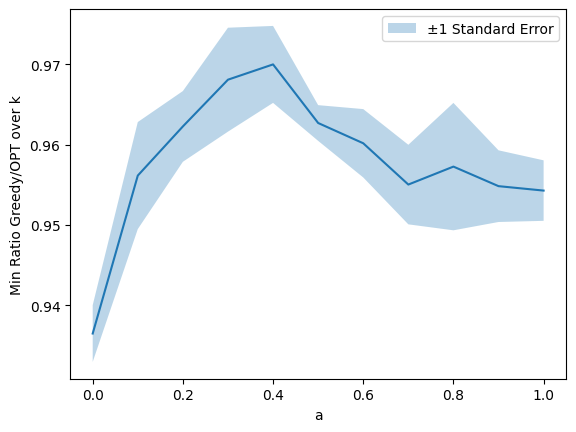
\includegraphics[width=\linewidth,height=0.78\textheight,keepaspectratio]{arxiv2604-24884v1-image-01.png}\par

Figure 1: The computation is carried out for $n=m=100$ and the ratio between the value of Greedy and Opt is calculated by averaging over $50$ runs. Opt was implemented in Python using Gurobi to solve the integer program. The shaded region depicts the standard error for our estimation.





\par\medskip\noindent\textbf{Appendix B Generalization Of Technical Tools}\par




In this section, we show that our main techniques from the proof of Theorems 1 and 2, can be used in a more general random model that allows different number of nodes on each side of the bipartite graph as well as non-uniform degrees for the left nodes.\par



% SOURCE-ID Thmdefinition2


\par\medskip\noindent\textbf{\textbf{Definition 2}\textbf{.}}\par



\emph{Let $n,m\in\mathbbm{N}$ and $d\in[m]$. The random model GenR($n,m,d_{1},\dots,d_{n}$) constructs a random bipartite graph $\mathcal{B}=\left(L,R,\mathcal{E}\right)$ such that the number of nodes is $|L|=n,|R|=m$ and the edges $\mathcal{E}$ are such that $N(u_{i})\in\binom{R}{d_{i}}$ is selected uniformly and independently for all $i\in[n]$.}\par



% END-SOURCE-ID Thmdefinition2



Notice that, GenR generalizes LRR and ULRR.\par




\par\medskip\noindent\textbf{B.1 Lower Bound By Differential Equation Method}\par




The following lemma shows that this algorithm is equivalent to Greedy for arbitrary $d$-left-regular bipartite graphs.\par



% SOURCE-ID Thmlemma12


\par\medskip\noindent\textbf{\textbf{Lemma 12}\textbf{.}}\par



\emph{Let $B=(L,R,E)$ be a $d$-left-regular bipartite graph.
Let $P_{t}=\max\{p\in[d]:|\mathcal{A}^{p}_{0}|\leq t\}$
and $I_{t}=\min\{i\in[n]:|\mathcal{A}^{P_{t}}_{i}|\geq t\}$.
Then $A^{p}_{i}=G_{t}$ for all $(p,i)\in\{(p^{\prime},i^{\prime}):p^{\prime}=P_{t},I_{t}\leq i^{\prime}\leq n\text{ or }P_{t+1}<p^{\prime}<P_{t},i^{\prime}\in[n]\text{ or }p^{\prime}=P_{t+1},0\leq i^{\prime}<I_{t+1}\}$ and $t\in[k]$.}\par



% END-SOURCE-ID Thmlemma12



\par\medskip\noindent\textbf{Proof.}\par



Notice that $I_{t}$ is by definition the iteration on which AcceptReject accepts the $t$-th node in phase $P_{t}$ and the additional nodes are never accepted.
We start by showing that $\mathcal{A}^{P_{t}}_{I_{t}}=\mathcal{G}_{t}$ by induction on $t$.
For $t=1$, we have that:\par


\[\begin{gathered}
\displaystyle|N(u_{1})\setminus N(\mathcal{G}_{0})|=|N(u_{1})\setminus N(\mathcal{A}^{d}_{0})|=d,
\end{gathered}\]


where the first equality is due to $\mathcal{G}_{0}=\mathcal{A}^{d}_{0}=\emptyset$.
Therefore $\mathcal{A}^{d}_{1}=\{u_{1}\}$ since on iteration $1$ it will accept $u_{1}$ and $\mathcal{G}_{1}=\{u_{1}\}$ since among all the nodes with contribution $d$, it has the lowest index.
For the inductive step $t=t_{0}+1$, let $u_{g}$ be the node such that $\mathcal{G}_{t_{0}+1}\setminus\mathcal{G}_{t_{0}}=\{u_{g}\}$.
By definition of Greedy that implies:\par


\[\begin{gathered}
\displaystyle g=\min\{i\in[n]:|N(u_{i})\setminus N(\mathcal{G}_{t_{0}})|\geq|N(u_{i^{\prime}})\setminus N(\mathcal{G}_{t_{0}})|,\forall i^{\prime}\in[n]\}.
\end{gathered}\]


Also let $u_{a}$ be the node such that $\mathcal{A}^{P_{t_{0}+1}}_{I_{t_{0}+1}}\setminus\mathcal{A}^{P_{t_{0}}}_{I_{t_{0}}}=\{u_{a}\}$ and we have that:\par


\[\begin{gathered}
\displaystyle|N(u_{a})\setminus N(\mathcal{A}^{P_{t_{0}}}_{I_{t_{0}}})|=|N(u_{a})\setminus N(\mathcal{G}_{t_{0}})|\leq|N(u_{g})\setminus N(\mathcal{G}_{t_{0}})|=|N(u_{g})\setminus N(\mathcal{A}^{P_{t_{0}}}_{I_{t_{0}}})|,
\end{gathered}\]


where the equality is by inductive hypothesis $\mathcal{A}^{P_{t_{0}}}_{I_{t_{0}}}=\mathcal{G}_{t_{0}}$ and the inequality by (*).
Assume towards a contradiction that $|N(u_{a})\setminus N(\mathcal{A}^{P_{t_{0}}}_{I_{t_{0}}})|<|N(u_{g})\setminus N(\mathcal{A}^{P_{t_{0}}}_{I_{t_{0}}})|$, so $u_{a}$ is accepted on phase $|N(u_{a})\setminus N(\mathcal{A}^{P_{t_{0}}}_{I_{t_{0}}})|$, which is later than phase $|N(u_{g})\setminus N(\mathcal{A}^{P_{t_{0}}}_{I_{t_{0}}})|$ and implies that AcceptReject rejected $u_{g}$ on phase $|N(u_{g})\setminus N(\mathcal{A}^{P_{t_{0}}}_{I_{t_{0}}})|$.
Overall we have that:\par


\[\begin{gathered}
\displaystyle|N(u_{a})\setminus N(\mathcal{A}^{P_{t_{0}}}_{I_{t_{0}}})|=|N(u_{g})\setminus N(\mathcal{A}^{P_{t_{0}}}_{I_{t_{0}}})|.
\end{gathered}\]


Assume towards a contradiction that $a\neq g$.
We start with the case $a<g$ which contradicts the minimality of $g$ in (*) due to (***).
On the other hand, if $a>g$, $u_{g}$ was reached in an earlier iteration of AcceptReject and must have been rejected in phase $|N(u_{a})\setminus N(\mathcal{A}^{P_{t_{0}}}_{I_{t_{0}}})|$ which is a contradiction by (***).
Overall we have that:\par


\[\begin{gathered}
\displaystyle\mathcal{A}^{P_{t_{0}+1}}_{I_{t_{0}+1}}=\mathcal{A}^{P_{t_{0}}}_{I_{t_{0}}}\cup\{u_{a}\}=\mathcal{A}^{P_{t_{0}}}_{I_{t_{0}}}\cup\{u_{g}\}=\mathcal{G}_{t_{0}}\cup\{u_{g}\}=\mathcal{G}_{t_{0}+1},
\end{gathered}\]


where the first equality is by definition of $P_{t},I_{t}$, the second due to $g=a$, the third is by inductive hypothesis and the fourth by definition of $u_{g}$.
This concludes the induction and in order to obtain the statement note that for any $(p,i)\in\{(p^{\prime},i^{\prime}):p^{\prime}=P_{t},I_{t}\leq i^{\prime}\leq n\text{ or }P_{t+1}<p^{\prime}<P_{t},i^{\prime}\in[n]\text{ or }p^{\prime}=P_{t+1},0\leq i^{\prime}<i_{t+1}\}$ we have that $\mathcal{A}^{p}_{i}=\mathcal{A}^{P_{t}}_{I_{t}}$ since no node is accepted in these iterations.
\ensuremath{\blacksquare}\par





\par\medskip\noindent\textbf{B.1.1 Number of accepts in first phase}\par




In the following lemma we calculate the accepts of phase 1 by using the differential equation method.\par



% SOURCE-ID Thmlemma13


\par\medskip\noindent\textbf{\textbf{Lemma 13}\textbf{.}}\par



\emph{Let $n,m\in\mathbbm{N}$, $d\in[m],k\in[n]$ and draw bipartite graph $\mathcal{B}=(L,R,\mathcal{E})$ from random model $\textsc{GenR}(n,m,d,\dots,d)$.
Also let $t^{*}_{d}=\left(1-\left(1+\frac{nd(d-1)}{m}\right)^{-\frac{1}{d-1}}\right)\cdot\frac{m}{d}$ and $\delta=3e^{\frac{nd^{2}}{m}}\cdot\sqrt{8n\log{2n}}$.
Then $|t_{d}-t^{*}_{d}|\leq\delta$ with probability at $1-\frac{1}{n}$ for all $m\geq 2d^{2}$.}\par



% END-SOURCE-ID Thmlemma13



\par\medskip\noindent\textbf{Proof.}\par



Due to the equivalence between AcceptReject and Greedy Lemma 12, on any graph $B=(L,R,E)$ we have $t_{d}=|\mathcal{A}^{d}_{n}|$, since at the end of phase $d$, AcceptReject has accepted all the nodes with marginal contribution $d$. Therefore, it suffices to estimate $|\mathcal{A}^{d}_{n}|$. Towards this end we define $Y(i)=|\mathcal{A}^{d}_{i}|$, i.e. the number of accepted nodes on iteration $i$ of phase $d$ and we have:\par


\[\begin{gathered}
\displaystyle\E\left[Y(i+1)-Y(i)\middle|Y(i)\right]=\E\left[\mathbbm{1}\{u_{i+1}\text{ accepted }\}\middle|Y(i)\right]=\Pr\left[u_{i+1}\text{ accepted }\middle|Y(i)\right]=\frac{\binom{m-Y(i)d}{d}}{\binom{m}{d}},
\end{gathered}\]


where the last equality is because $u_{i+1}$ is accepted only if $|N(u_{i+1})\setminus N(\mathcal{A}^{d}_{i})|=d$. But since $|N(\mathcal{A}^{d}_{i})|=Y(i)\cdot d$ and $N(u_{i+1})$ are selected uniformly at random from the $m$ right nodes, the only way $u_{i+1}$ was accepted was if it sampled $d$ nodes from the $m-Y(i)\cdot d$ remaining.
We can now show one by one that the assumptions of the differential equation hold:\par


\begin{enumerate}


\item[] 1. 


Trend Hypothesis: $\bigl|\E\left[Y(i+1)-Y(i)\middle|Y(i)\right]-\left(1-\frac{nd}{m}\frac{Y(i)}{n}\right)^{d}\bigr|\leq\frac{2d^{2}}{m}$ by Lemma 14 for $r=m-Y(i)d$ since $m\geq 2d^{2}$,\par




\item[] 2. 


Lipschitz Hypothesis: $F(y)=\left(1-\frac{nd}{m}y\right)^{d}$ is $\frac{nd^{2}}{m}$-Lipschitz since:\par


\[\begin{gathered}
\displaystyle\bigl|F(y_{1})-F(y_{2})\bigr| \displaystyle=\bigl|\left(1-\frac{nd}{m}y_{1}\right)^{d}-\left(1-\frac{nd}{m}y_{2}\right)^{d}\bigr| \\
\displaystyle=\frac{nd}{m}\cdot\bigl|\left(\left(1-\frac{nd}{m}y_{1}\right)^{d-1}+\dots+\left(1-\frac{nd}{m}y_{2}\right)^{d-1}\right)\bigr|\cdot\bigl|y_{2}-y_{1}\bigr| \\
\displaystyle\leq\frac{nd}{m}\cdot\bigl|1+\dots+1\bigr|\cdot\bigl|y_{2}-y_{1}\bigr| \\
\displaystyle=\frac{nd^{2}}{m}\cdot\bigl|y_{1}-y_{2}\bigr|,
\end{gathered}\]




\item[] 3. 


Boundedness Hypothesis: $\bigl|Y(i+1)-Y(i)\bigr|\leq 1$ as only node $u_{i+1}$ can be accepted on iteration $i+1$,\par




\item[] 4. 


Initial Condition: $Y(0)=\hat{y}=0$ so any $\lambda\geq\frac{2}{n}\geq\frac{d^{2}}{m}\min\{T,\frac{m}{nd^{2}}\}+\frac{R}{n}=\frac{d^{2}}{m}\min\{1,\frac{m}{nd^{2}}\}+\frac{1}{n}$ works. We choose $\lambda=\sqrt{\frac{8\log{(2n)}}{n}}$.\par




\end{enumerate}




Model $Y(i)$ by $ny\left(\frac{i}{n}\right)$ and we obtain the following differential equation:\par


\[\begin{gathered}
\displaystyle y^{\prime}(t)=\left(1-\frac{nd}{m}\cdot y(t)\right)^{d},\ y(0)=0.
\end{gathered}\]


By Lemma 16 with probability $1-2e^{-n\lambda^{2}/8T}=1-\frac{1}{n}$ we have that:\par


\[\begin{gathered}
\displaystyle\bigl|Y(i)-ny(i/n)\bigr|<3e^{\frac{nd^{2}}{m}T}\cdot\lambda n=3e^{\frac{nd^{2}}{m}}\cdot\sqrt{8n\log(2n)}.
\end{gathered}\]


\ensuremath{\blacksquare}\par





In the following lemma we approximate the probability of success.\par



% SOURCE-ID Thmlemma14


\par\medskip\noindent\textbf{\textbf{Lemma 14}\textbf{.}}\par



\emph{Let $d\in\mathbbm{N}$, $m\geq 2d^{2}$, $r\in[m]$
then $|\binom{r}{d}/\binom{m}{d}-\left(\frac{r}{m}\right)^{d}|\leq\frac{2d^{2}}{m}$.}\par



% END-SOURCE-ID Thmlemma14



\par\medskip\noindent\textbf{Proof.}\par



We start by showing the upper bound:\par


\[\begin{gathered}
\displaystyle\frac{\binom{r}{d}}{\binom{m}{d}}=\frac{r(r-1)\cdots(r-d+1))}{m(m-1)\cdots(m-d+1)}=\prod_{i=0}^{d-1}\left(\frac{r-i}{m-i}\right)\leq\left(\frac{r}{m}\right)^{d}.
\end{gathered}\]


We proceed to show the lower bound:\par


\[\begin{gathered}
\displaystyle\frac{\binom{r}{d}}{\binom{m}{d}}=\prod_{i=0}^{d-1}\left(\frac{r-i}{m-i}\right)=\prod_{i=0}^{d-1}\left(\frac{r}{m}\cdot\frac{1-\frac{i}{r}}{1-\frac{i}{m}}\right) \displaystyle=\left(\frac{r}{m}\right)^{d}\cdot\prod_{i=0}^{d-1}\left(1-\frac{i(m-r)}{r(m-i)}\right) \\
\displaystyle\geq\left(\frac{r}{m}\right)^{d}\cdot\left(1-\sum_{i=0}^{d-1}\frac{i(m-r)}{r(m-i)}\right) \\
\displaystyle\geq\left(\frac{r}{m}\right)^{d}\cdot\left(1-\frac{m-r}{r(m-d)}\cdot\sum_{i=0}^{d-1}i\right) \\
\displaystyle=\left(\frac{r}{m}\right)^{d}\cdot\left(1-\frac{m-r}{r(m-d)}\cdot\frac{d(d-1)}{2}\right) \\
\displaystyle=\left(\frac{r}{m}\right)^{d}-\left(\frac{r}{m}\right)^{d-1}\cdot\frac{m-r}{m-d}\cdot\frac{d^{2}}{2m} \\
\displaystyle\geq\left(\frac{r}{m}\right)^{d}-\frac{m}{m-d}\cdot\frac{d^{2}}{2m} \\
\displaystyle\geq\left(\frac{r}{m}\right)^{d}-\frac{2d^{2}}{m},
\end{gathered}\]


where the first inequality is due to $\prod_{i=0}^{d-1}(1-x_{i})\geq 1-\sum_{i=0}^{d-1}x_{i}$ for all $x_{i}\in[0,1]$, the second inequality is due to $m-i\geq m-d$ for all $i\in[d-1]$, the third inequality is due to $\frac{r}{m}\leq 1$ and the fourth inequality is because $d\leq\sqrt{m}$, so $\frac{m}{m-d}\leq\frac{m}{m-\sqrt{m}}=\frac{1}{1-1/\sqrt{m}}\leq 4$ for all $m\geq 2d^{2}\geq 2$.
\ensuremath{\blacksquare}\par





In the following lemma we solve the main differential equation.\par



% SOURCE-ID Thmlemma15


\par\medskip\noindent\textbf{\textbf{Lemma 15}\textbf{.}}\par



\emph{The unique solution of $y^{\prime}(t)=\left(1-\frac{nd}{m}\cdot y(t)\right)^{d}$ with initial condition $y(0)=0$ is
$y(t)=\frac{m}{nd}\cdot\left(1-\left(1+\frac{nd(d-1)}{m}\cdot t\right)^{-\frac{1}{d-1}}\right)$.}\par



% END-SOURCE-ID Thmlemma15



\par\medskip\noindent\textbf{Proof.}\par



We rewrite the differential equation in the following form:\par


\[\begin{gathered}
\displaystyle\frac{y^{\prime}(t)}{\left(1-\frac{nd}{m}\cdot y(t)\right)^{d}}=1,\ y(0)=0.
\end{gathered}\]


By integrating both sides of Equation (1) in $[0,t]$ we have:\par


\[\begin{gathered}
\displaystyle\frac{\left(1-\frac{nd}{m}y(t)\right)^{-(d-1)}}{\frac{nd(d-1)}{m}}-\frac{1}{\frac{nd(d-1)}{m}}=t.
\end{gathered}\]


We obtain the statement by solving for $y(t)$.
\ensuremath{\blacksquare}\par






\par\medskip\noindent\textbf{B.1.2 Differential Equation Method}\par



% SOURCE-ID Thmlemma16


\par\medskip\noindent\textbf{\textbf{Lemma 16}\textbf{ }(Theorem 2 in [30])\textbf{.}}\par



\emph{Given integers $a,n\geq 1$,
a bounded domain $\mathcal{D}\subseteq\mathbb{R}^{a+1}$,
functions $(F_{k})_{1\leq k\leq a}$ with $F_{k}:\mathcal{D}\to\mathbb{R}$,
and $\sigma$-fields $\mathcal{F}_{0}\subseteq\mathcal{F}_{1}\subseteq\cdots$,
suppose that the random variables $((Y_{k}(i))_{1\leq k\leq a}$ are $\mathcal{F}_{i}$-measurable for $i\geq 0$.
Furthermore, assume that, for all $i\geq 0$ and $1\leq k\leq a$, the following
conditions hold whenever $(i/n,Y_{1}(i)/n,...,Y_{a}(i)/n)\in\mathcal{D}$:}\par


\begin{enumerate}


\item[] (i) 


$\bigl|\E\left(Y_{k}(i+1)-Y_{k}(i)\mid\mathcal{F}_{i}\right)-F_{k}\left(i/n,Y_{1}(i)/n,...,Y_{a}(i)/n\right)\bigr|\leq\delta$\emph{,
where the function }$F_{k}$\emph{ is }$L$\emph{-Lipschitz-continuous on }$\mathcal{D}$\emph{  }(the ‘Trend hypothesis’ and ‘Lipschitz hypothesis’)\emph{,}\par




\item[] (ii) 


$\bigl|Y_{k}(i+1)-Y_{k}(i)\bigr|\leq\beta$\emph{  }(the ‘Boundedness hypothesis’)\emph{,}\par




\end{enumerate}


\emph{and that the following condition holds initially:}\par


\begin{enumerate}


\item[] (iii) 


$\max_{1\leq k\leq a}\bigl|Y_{k}(0)-\hat{y}_{k}n\bigr|\leq\lambda n$\emph{ for some }$(0,\hat{y}_{1},\ldots,\hat{y}_{a})\in\mathcal{D}$\emph{
 }(the ‘Initial condition’)\emph{.}\par




\end{enumerate}


\emph{Then there are $R=R(\mathcal{D},(F_{k})_{1\leq k\leq a},L)\in[1,\infty)$ and $T=T(\mathcal{D})\in(0,\infty)$ such that,
whenever $\lambda\geq\delta\min\{T,L^{-1}\}+R/n$,
with probability at least $1-2ae^{-n\lambda^{2}/(8T\beta^{2})}$ we have}\par


\[\begin{gathered}
\max_{0\leq i\leq\sigma n}\max_{1\leq k\leq a}\bigl|Y_{k}(i)-y_{k}\left(\tfrac{i}{n}\right)n\bigr|\;<\;3e^{LT}\lambda n,
\end{gathered}\]


\emph{where $(y_{k}(t))_{1\leq k\leq a}$ is the unique solution to the system of differential equations}\par


\[\begin{gathered}
y^{\prime}_{k}(t)=F_{k}\left(t,y_{1}(t),\ldots,y_{a}(t)\right)\quad\text{ with }\quad y_{k}(0)=\hat{y}_{k}\qquad\text{for~$1\leq k\leq a$,}
\end{gathered}\]


\emph{and $\sigma=\sigma(\hat{y}_{1},\ldots\hat{y}_{a})\in[0,T]$ is any choice of $\sigma\geq 0$ with the property
that $(t,y_{1}(t),\ldots y_{a}(t))$ has $\ell^{\infty}$-distance at least $3e^{LT}\lambda$
from the boundary of $\mathcal{D}$ for all $t\in[0,\sigma)$.}\par



% END-SOURCE-ID Thmlemma16





\par\medskip\noindent\textbf{B.2 Fixed Set Lower Bound}\par




We proceed to show that Greedy achieves higher value than the fixed set of the $k$ nodes with the highest degrees, $H_{k}$. First, we calculate the expected value of this set.\par



% SOURCE-ID Thmlemma17


\par\medskip\noindent\textbf{\textbf{Lemma 17}\textbf{.}}\par



\emph{Let $m,n\in\mathbbm{N}$, $m\geq d_{1}\geq\dots\geq d_{n}\geq 0,k\in[n]$ and draw bipartite graph $\mathcal{B}=(L,R,\mathcal{E})$ from random model $\textsc{GenR}(n,m,d_{1},\dots,d_{n})$.
Then $\E[|N(H_{k})|]=\left(1-\prod_{i=1}^{k}\left(1-\frac{d_{i}}{m}\right)\right)\cdot m\geq\left(1-e^{-\frac{\sum_{i=1}^{k}d_{i}}{m}}\right)\cdot m$.}\par



% END-SOURCE-ID Thmlemma17



\par\medskip\noindent\textbf{Proof.}\par



Notice that $H_{k}$ covers node $v_{j}$ as long as at least one of its nodes covers $v_{j}$, so for all $j\in[m]$:\par


\[\begin{gathered}
\displaystyle\Pr\left[v_{j}\in N(H_{k})\right]=1-\prod_{u_{i}\in H_{k}}{\left(1-\Pr\left[v_{j}\in N(u_{i})\right]\right)}=1-\prod_{i=1}^{k}{\left(1-\frac{d_{i}}{m}\right)}\geq 1-e^{-\frac{\sum_{i=1}^{k}d_{i}}{m}}.
\end{gathered}\]


We have that:\par


\[\begin{gathered}
\displaystyle\E\left[|N(H_{k})|\right]=\E\left[\sum_{j\in[m]}{\mathbbm{1}\{v_{j}\in N(H_{k})\}}\right]=\sum_{j\in[m]}{\Pr[v_{j}\in N(H_{k})]}=\Pr\left[v_{1}\in N(H_{k})\right]\cdot m,
\end{gathered}\]


where the first equality is by definition, the second equality is by linearity of expectation and the third equality because the probabilities are equal for all $j\in[m]$. Then the statement follows.
\ensuremath{\blacksquare}\par





We introduce notation that is useful for the proofs in this section.
Informally, $M_{t}(S)$ is the set of the $t$ nodes with the highest marginal contributions to a set of nodes $S$.
Let $S\subseteq L$ and define:\par


\[\begin{gathered}
\displaystyle u^{(i)}=\begin{cases}\arg\max\{|N(u)\setminus N(S)|:u\in L\setminus S\}&\text{ if }i=1\\
\arg\max\{|N(u)\setminus N(S)|:u\in L\setminus\left(S\cup\{u^{(1)},\dots,u^{(i-1)}\}\right)\}&\text{ otherwise }\end{cases},
\end{gathered}\]


where we abuse notation so that $\arg\max$ breaks ties like Greedy, which uniquely defines $u^{(i)}$.
Then we define $M_{t}(S)=\{u^{(1)},u^{(2)},\dots,u^{(t)}\}$.
Now we define the hybrid algorithm:\par


\[\begin{gathered}
\displaystyle Y^{t}=G_{t}\cup M_{k-t}(G_{t}).
\end{gathered}\]


Notice that $Y^{k}=G_{k}$ while $Y^{0}=H_{k}$.\par



% SOURCE-ID Thmlemma18


\par\medskip\noindent\textbf{\textbf{Lemma 18}\textbf{.}}\par



\emph{Let $m,n\in\mathbbm{N}$, $m\geq d_{1}\geq\dots\geq d_{n}\geq 1$, $k\in[n]$ and draw graph $\mathcal{B}$ from GenR$(n,m,d_{1},\dots,d_{n})$. Then $\E[|N(\mathcal{G}_{k})|]\geq\E[|N(H_{k})|]$ for any $n,m,k$.}\par



% END-SOURCE-ID Thmlemma18



\par\medskip\noindent\textbf{Proof.}\par



We claim that $\E[|N(\mathcal{Y}^{t})|]\geq\E[|N(\mathcal{Y}^{t-1})|]$ for any $t\in[k]$.
Assuming it holds we apply it repeatedly and we have that:\par


\[\begin{gathered}
\displaystyle\E[|N(\mathcal{G}_{k})|]=\E[|N(\mathcal{Y}^{k})|]\geq\E[|N(\mathcal{Y}^{k-1})|]\geq\dots\geq\E[|N(\mathcal{Y}^{0})|]=\E[|N(H_{k})|],
\end{gathered}\]


which implies the statement.
For the rest of the proof, we fix $t$ and focus on showing the claim.
We denote $\mathcal{M}_{k-t}(\mathcal{G}_{t})=\{u^{(1)},\dots,u^{(k-t)}\}$ and $\mathcal{M}_{k-t+1}(\mathcal{G}_{t-1})=\{u^{\prime(1)},\dots,u^{\prime(k-t+1)}\}$.
Let $X_{l}=N(u^{(\ell)})\setminus N(\mathcal{G}_{t})$ and $Y_{\ell}=N(u^{\prime(\ell+1)})\setminus N(\mathcal{G}_{t})$ for all $\ell\in[k-t]$.
For the left-hand side we have that:\par


\[\begin{gathered}
\displaystyle|N(\mathcal{Y}^{t})| \displaystyle=|N(\mathcal{G}_{t}\cup\mathcal{M}_{k-t}(\mathcal{G}_{t}))| \\
\displaystyle=|N(\mathcal{G}_{t})\cup N(\mathcal{M}_{k-t}(\mathcal{G}_{t}))| \\
\displaystyle=|N(\mathcal{G}_{t})\cup N(\{u^{(1)},\dots,u^{(i)}\})| \\
\displaystyle=|N(\mathcal{G}_{t})|+|N(\{u^{(1)},\dots,u^{(k-t)}\})\setminus N(\mathcal{G}_{t})| \\
\displaystyle=|N(\mathcal{G}_{t})|+|\bigcup_{\ell=1}^{k-t}{N(u^{(\ell)})\setminus N(\mathcal{G}_{t})}| \\
\displaystyle=|N(\mathcal{G}_{t})|+|\bigcup_{\ell=1}^{k-t}{X_{\ell}}|,
\end{gathered}\]


where the first line is by definition of $\mathcal{Y}^{t}$, the second line is due to $N(A\cup B)=N(A)\cup N(B)$ for any sets of nodes $A,B\subseteq L$, the third line is by definition of $\mathcal{M}_{k-t}(\mathcal{G}_{t})$, the fourth line is by splitting the cardinality of the union with the sum of of cardinalities of disjoint sets, the fifth line is by $N(A\cup B)=N(A)\cup N(B)$ and the sixth line is by definition of $X_{\ell}$.
For the right-hand side we have that:\par


\[\begin{gathered}
\displaystyle|N(\mathcal{Y}^{t-1})| \displaystyle=|N(\mathcal{G}_{t-1}\cup\mathcal{M}_{k-t+1}(\mathcal{G}_{t-1}))| \\
\displaystyle=|N((\mathcal{G}_{t-1}\cup\{u^{\prime(1)}\})\cup(\mathcal{M}_{k-t+1}(\mathcal{G}_{t-1})\setminus\{u^{\prime(1)}\}))| \\
\displaystyle=|N(\mathcal{G}_{t}\cup(\mathcal{M}_{k-t+1}(\mathcal{G}_{t-1})\setminus\{u^{\prime(1)}\}))| \\
\displaystyle=|N(\mathcal{G}_{t})\cup N(\mathcal{M}_{k-t+1}(\mathcal{G}_{t-1})\setminus\{u^{\prime(1)}\})| \\
\displaystyle=|N(\mathcal{G}_{t})\cup N(\{u^{\prime(2)},\dots,u^{\prime(k-t+1)}\})| \\
\displaystyle=|N(\mathcal{G}_{t})|+|N(\{u^{\prime(2)},\dots,u^{\prime(k-t+1)}\})\setminus N(\mathcal{G}_{t})| \\
\displaystyle=|N(\mathcal{G}_{t})|+|\bigcup_{\ell=1}^{k-t}{N(u^{\prime(\ell+1)})\setminus N(\mathcal{G}_{t})}| \\
\displaystyle=|N(\mathcal{G}_{t})|+|\bigcup_{\ell=1}^{i=k-t}{Y_{\ell}}|,
\end{gathered}\]


where the first equality is by definition of $\mathcal{Y}^{t-1}$, the second follows by removing $u^{\prime(1)}$ from the right set and adding it to the left which does not affect the union, the third is due to $\mathcal{G}_{t}=\mathcal{G}_{t-1}\cup\{u^{\prime(1)}\}$ which follows by definition of $\mathcal{G}_{t-1}$ and $u^{\prime(1)}$, the fourth is due to $N(A\cup B)=N(A)\cup N(B)$ for any sets of nodes $A,B\subseteq L$, the fifth is by definition of $\mathcal{M}_{k-t+1}(\mathcal{G}_{t-1})$, the sixth is by splitting the cardinality of the union with the sum of of cardinalities of disjoint sets and the seventh is by $N(A\cup B)=N(A)\cup N(B)$.\par




Let $A=\{a_{1},\dots,a_{t}\}\subseteq L$, $T\subseteq R$ and $D_{i}\in[d_{i}]$ for all $i$ such that $u_{i}\in L\setminus A$ arbitrarily. Also let $\mathscr{F}$ be the family of all edge sets $E$ such that $\mathcal{G}_{t}=A,N(A)=T,|N(u_{i})\setminus T|=D_{i}$ for all $i$ such that $u_{i}\in L\setminus A$.
We now show that that:\par


\[\begin{gathered}
\displaystyle\E\left[|\bigcup_{\ell=1}^{k-t}{X_{\ell}}|\mid\mathcal{E}\in\mathscr{F}\right]\geq\E\left[|\bigcup_{\ell=1}^{k-t}{Y_{\ell}}|\mid\mathcal{E}\in\mathscr{F}\right],
\end{gathered}\]


by using Lemma 26, which requires the following:\par


\begin{enumerate}


\item[] 1. 


$X_{1},\dots,X_{k-t}$ and $Y_{1},\dots,Y_{k-t}$ are pairwise independent, conditionally on $\mathscr{F}$,\par




\item[] 2. 


$X_{\ell},Y_{\ell}$ uniform in $R\setminus N(\mathcal{G}_{t})$ for all $\ell\in[k-t]$, conditionally on $\mathscr{F}$,\par




\item[] 3. 


$\E[|X_{\ell}|\mid\mathcal{E}\in\mathscr{F}]\geq\E[|Y_{\ell}|\mid\mathcal{E}\in\mathscr{F}]$.\par




\end{enumerate}


For the first point, by Lemma 20 we have that $X_{1},\dots,X_{i}$ are pairwise independent and $Y_{1},\dots Y_{i}$ are pairwise independent.
For the second point, by Lemma 19
we have that $X_{\ell}$ and $Y_{\ell}$ are uniform in $R\setminus N(\mathcal{G}_{t})$ for all $\ell\in[k-t]$.
For the third point, notice that:\par


\[\begin{gathered}
\displaystyle\E[|X_{\ell}|\mid\mathcal{E}\in\mathscr{F}]=\E[|N(u^{(\ell)})\setminus N(\mathcal{G}_{t})|\mid\mathcal{E}\in\mathscr{F}] \displaystyle\geq\E[|N(u^{\prime(\ell+1)})\setminus N(\mathcal{G}_{t})|\mid\mathcal{E}\in\mathscr{F}] \\
\displaystyle=\E[|Y_{\ell}|\mid\mathcal{E}\in\mathscr{F}],
\end{gathered}\]


where the inequality follows because right after iteration $t$, $u^{(\ell)}$
has higher marginal contribution to $\mathcal{G}_{t}$ than $u^{\prime(\ell+1)}$, as the former is by definition the $\ell$-th highest marginal contribution after removing $|N(\mathcal{G}_{t})|$, while the latter is by definition the $\ell+1$-th highest marginal contribution after removing $|N(\mathcal{G}_{t-1})|$.
Overall we have that:\par


\[\begin{gathered}
\displaystyle\E[|N(\mathcal{Y}^{t})|\mid\mathcal{E}\in\mathscr{F}] \displaystyle=\E[|N(\mathcal{G}_{t})|\mid\mathcal{E}\in\mathscr{F}]+\E[|\bigcup_{\ell=1}^{k-t}{X_{\ell}}|\mid\mathcal{E}\in\mathscr{F}] \\
\displaystyle=|T|+\E[|\bigcup_{\ell=1}^{k-t}{X_{\ell}}|\mid\mathcal{E}\in\mathscr{F}] \\
\displaystyle\geq|T|+\E[|\bigcup_{\ell=1}^{k-t}{Y_{\ell}}|\mid\mathcal{E}\in\mathscr{F}] \\
\displaystyle=\E[|N(\mathcal{G}_{t})|\mid\mathcal{E}\in\mathscr{F}]+\E[|\bigcup_{\ell=1}^{k-t}{Y_{\ell}}|\mid\mathcal{E}\in\mathscr{F}] \\
\displaystyle=\E[|N(\mathcal{Y}^{t-1})|\mid\mathcal{E}\in\mathscr{F}],
\end{gathered}\]


where the first line is due to Equation (1), the second line is by definition of $\mathscr{F}$, the third line is due to Equation (3), the fourth line is by definition of $\mathscr{F}$ and the fifth line is due to Equation (2).
Since the claim holds for any $A,T,(D_{i})_{i:u_{i}\in L\setminus A}$, it also holds unconditionally.
\ensuremath{\blacksquare}\par





\par\medskip\noindent\textbf{B.2.1 Structural Lemmas}\par




We show some structural lemmas that help us prove Lemma 18. In this paragraph, when the bipartite graph is clear from context, we use $G_{t}(E)$ to indicate the output of Greedy when it is run on edge set $E$.\par



% SOURCE-ID Thmlemma19


\par\medskip\noindent\textbf{\textbf{Lemma 19}\textbf{ }(Uniform marginal contributions)\textbf{.}}\par



\emph{Let $m\geq d_{1}\geq\dots\geq d_{n}\geq 1$. Draw graph $\mathcal{B}$ from random model $\textsc{GenR}(n,m,d_{1},\dots,d_{n})$ with edge set $\mathcal{E}$.
Also define the following arbitrarily:}\par


\begin{enumerate}


\item[] 1. 


$A=\{a_{1},\dots,a_{t}\}\subseteq L$\emph{,}\par




\item[] 2. 


$T\subseteq R$\emph{ such that }$\min_{i}{d_{i}}\leq|T|\leq\min\{\sum_{i=1}^{t}d_{i},m\}$\emph{,}\par




\item[] 3. 


$D_{i}\in[d_{i}]$\emph{ for all }$i$\emph{ such that }$u_{i}\in L\setminus A$\emph{,}\par




\item[] 4. 


$u_{x}\in L\setminus A$\emph{.}\par




\end{enumerate}


\emph{Let $\mathscr{F}=\{E\subseteq L\times R:G_{t}(E)=A,N_{E}(A)=T,|N_{E}(u_{i})\setminus T|=D_{i}\ \forall i\text{ s.t. }u_{i}\in L\setminus A\}$.
Then we have that:}\par


\[\begin{gathered}
\displaystyle\Pr\left[N_{\mathcal{E}}(u_{x})\setminus T=X\mid\mathcal{E}\in\mathscr{F}\right]=\Pr\left[N_{\mathcal{E}}(u_{x})\setminus T=X^{\prime}\mid\mathcal{E}\in\mathscr{F}\right],
\end{gathered}\]


\emph{for any $X,X^{\prime}\subseteq R\setminus T$ such that $|X|=|X^{\prime}|=D_{x}$.}\par



% END-SOURCE-ID Thmlemma19



\par\medskip\noindent\textbf{Proof.}\par



Let $E^{\prime}_{1}=\{u_{x}\}\times X$ and $E^{\prime}_{2}=\{u_{x}\}\times X^{\prime}$, then we have:\par


\[\begin{gathered}
\displaystyle\Pr[N_{\mathcal{E}}(u_{x})\setminus T=X\mid\mathcal{E}\in\mathscr{F}] \displaystyle=\Pr[\mathcal{E}_{\{u_{x}\}}=E^{\prime}_{1}\mid\mathcal{E}\in\mathscr{F}] \\
\displaystyle=\Pr[\mathcal{E}_{\{u_{x}\}}=E^{\prime}_{2}\mid\mathcal{E}\in\mathscr{F}] \\
\displaystyle=\Pr[N_{\mathcal{E}}(u_{x})\setminus T=X^{\prime}\mid\mathcal{E}\in\mathscr{F}],
\end{gathered}\]


where the first equality is due to $\mathcal{E}_{\{u_{x}\}}=\{(u_{x},v)\in\mathcal{E}:v\in R\setminus T\}$ and $E^{\prime}_{1}=\{u_{x}\}\times X$ so $\mathcal{E}_{\{x\}}=E^{\prime}_{1}$ is equivalent to $N_{\mathcal{E}}(x)\setminus T=X$, the second equality is due to Lemma 22 and the third equality is due to $\mathcal{E}_{\{u_{x}\}}=\{(u_{x},v)\in\mathcal{E}:v\in R\setminus T\}$ and $E^{\prime}_{2}=\{u_{x}\}\times X^{\prime}$ so $\mathcal{E}_{\{u_{x}\}}=E^{\prime}_{2}$ is equivalent to $N_{\mathcal{E}}(u_{x})\setminus T=X^{\prime}$.
\ensuremath{\blacksquare}\par




% SOURCE-ID Thmlemma20


\par\medskip\noindent\textbf{\textbf{Lemma 20}\textbf{ }(Independent marginal contributions)\textbf{.}}\par



\emph{Let $m\geq d_{1}\geq\dots\geq d_{n}\geq 1$. Draw graph $\mathcal{B}$ from random model $\textsc{GenR}(n,m,d_{1},\dots,d_{n})$ with edge set $\mathcal{E}$.
Also define the following arbitrarily:}\par


\begin{enumerate}


\item[] 1. 


$A=\{a_{1},\dots,a_{t}\}\subseteq L$\emph{,}\par




\item[] 2. 


$T\subseteq R$\emph{ such that }$\min_{i}{d_{i}}\leq|T|\leq\min\{\sum_{i=1}^{t}d_{i},m\}$\emph{,}\par




\item[] 3. 


$D_{i}\in[d_{i}]$\emph{ for all }$i$\emph{ such that }$u_{i}\in L\setminus A$\emph{,}\par




\item[] 4. 


$u_{x},u_{y}\in L\setminus A$\emph{.}\par




\end{enumerate}


\emph{Let $\mathscr{F}=\{E\subseteq L\times R:G_{t}(E)=A,N_{E}(A)=T,|N_{E}(u_{i})\setminus T|=D_{i}\ \forall i\text{ s.t. }u_{i}\in L\setminus A\}$.
Then we have that:}\par


\[\begin{gathered}
\displaystyle\Pr[N_{\mathcal{E}}(u_{x})\setminus T=X,N_{\mathcal{E}}(u_{y})\setminus T=Y\mid\mathcal{E}\in\mathscr{F}]= \displaystyle\Pr[N_{\mathcal{E}}(u_{x})\setminus T=X\mid\mathcal{E}\in\mathscr{F}] \\
\displaystyle\cdot\Pr[N_{\mathcal{E}}(u_{y})\setminus T=Y\mid\mathcal{E}\in\mathscr{F}],
\end{gathered}\]


\emph{for any $X,Y\subseteq R\setminus T$ and $|X|=D_{x},|Y|=D_{y}$.}\par



% END-SOURCE-ID Thmlemma20



\par\medskip\noindent\textbf{Proof.}\par



To obtain the statement we apply Lemma 27 on random sets $N_{\mathcal{E}}(u_{x})\setminus T,N_{\mathcal{E}}(u_{y})\setminus T$, so it suffices to show the following properties:\par


\begin{enumerate}


\item[] 1. 


$\Pr[N_{\mathcal{E}}(u_{x})\setminus T=X\mid\mathcal{E}\in\mathscr{F}]=\Pr[N_{\mathcal{E}}(u_{x})\setminus T=X^{\prime}\mid\mathcal{E}\in\mathscr{F}]$ for any $X,X^{\prime}\subseteq R\setminus T$ such that $|X|=|X^{\prime}|=D_{x}$,\par




\item[] 2. 


$\Pr[N_{\mathcal{E}}(u_{x})\setminus T=X,N_{\mathcal{E}}(u_{y})\setminus=Y\mid\mathcal{E}\in\mathscr{F}]=\Pr[N_{\mathcal{E}}(u_{x})\setminus T=X^{\prime},N_{\mathcal{E}}(u_{y})\setminus T=Y\mid\mathcal{E}\in\mathscr{F}]$, for any $X,X^{\prime},Y\subseteq R\setminus T$ such that $|X|=|X^{\prime}|=D_{x}$ and $|Y|=D_{y}$.\par




\end{enumerate}


Notice that the first property follows directly from Lemma 19.
We proceed to show the second property.
Let $E^{\prime}_{1}=\{u_{x}\}\times X\cup\{u_{y}\}\times Y$ and $E^{\prime}_{2}=\{u_{x}\}\times X^{\prime}\cup\{u_{y}\}\times Y$, then we have:\par


\[\begin{gathered}
\displaystyle\Pr[N_{\mathcal{E}}(u_{x})\setminus T=X,N_{\mathcal{E}}(u_{y})\setminus T=Y\mid\mathcal{E}\in\mathscr{F}] \displaystyle=\Pr[\mathcal{E}_{\{u_{x},u_{y}\}}=E^{\prime}_{1}\mid\mathcal{E}\in\mathscr{F}] \\
\displaystyle=\Pr[\mathcal{E}_{\{u_{x},u_{y}\}}=E^{\prime}_{2}\mid\mathcal{E}\in\mathscr{F}] \\
\displaystyle=\Pr[N_{\mathcal{E}}(u_{x})\setminus T=X^{\prime},N_{\mathcal{E}}(u_{y})\setminus T=Y\mid\mathcal{E}\in\mathscr{F}],
\end{gathered}\]


where the first equality is due to $\mathcal{E}_{\{u_{x},u_{y}\}}=\{(u,v)\in\mathcal{E}:u\in\{u_{x},u_{y}\},v\in R\setminus T\}$ and $E^{\prime}_{1}=\{u_{x}\}\times X\cup\{u_{y}\}\times Y$ so $\mathcal{E}_{\{u_{x},u_{y}\}}=E^{\prime}_{1}$ is equivalent to $N_{\mathcal{E}}(u_{x})\setminus T=X,N_{\mathcal{E}}(u_{y})\setminus T=Y$, the second equality is due to Lemma 22 and the third equality is due to $\mathcal{E}_{\{u_{x},u_{y}\}}=\{(u,v)\in\mathcal{E}:u\in\{u_{x},u_{y}\},v\in R\setminus T\}$ and $E^{\prime}_{2}=\{u_{x}\}\times X^{\prime}\cup\{u_{y}\}\times Y$ so $\mathcal{E}_{\{u_{x},u_{y}\}}=E^{\prime}_{2}$ is equivalent to $N_{\mathcal{E}}(u_{x})\setminus T=X^{\prime},\cup\{u_{y}\}\times Y$.
\ensuremath{\blacksquare}\par




% SOURCE-ID Thmlemma21


\par\medskip\noindent\textbf{\textbf{Lemma 21}\textbf{.}}\par



\emph{Let $m\geq d_{1}\geq\dots\geq d_{n}\geq 1$ and $\mathcal{B}\sim\textsc{GenR}(n,m,d_{1},\dots,d_{n})$ with edge set $\mathcal{E}$.
Also define the following arbitrarily:}\par


\begin{enumerate}


\item[] 1. 


$A=\{a_{1},\dots,a_{t}\}\subseteq L$\emph{,}\par




\item[] 2. 


$T\subseteq R$\emph{ such that }$\min_{i}{d_{i}}\leq|T|\leq\min\{\sum_{i=1}^{t}d_{i},m\}$\emph{,}\par




\item[] 3. 


$D_{i}\in[d_{i}]$\emph{ for all }$i$\emph{ such that }$u_{i}\in L\setminus A$\emph{,}\par




\item[] 4. 


$Z\subseteq L\setminus A$\emph{.}\par




\end{enumerate}


\emph{Let $\mathscr{F}=\{E\subseteq L\times R:G_{t}(E)=A,N_{E}(A)=T,|N_{E}(u_{i})\setminus T|=D_{i}\ \forall i\text{ s.t. }u_{i}\in L\setminus A\}$.
Also let $\mathcal{E}_{Z}=\{(u,v)\in\mathcal{E}:u\in Z,v\in R\setminus T\}$.
Then we have that:}\par


\[\begin{gathered}
\displaystyle\Pr\left[\mathcal{E}_{Z}=E^{\prime}_{1}\mid\mathcal{E}\in\mathscr{F}\right]=\Pr\left[\mathcal{E}_{Z}=E^{\prime}_{2}\mid\mathcal{E}\in\mathscr{F}\right],
\end{gathered}\]


\emph{for any $E^{\prime}_{1},E^{\prime}_{2}\subseteq Z\times(R\setminus T)$ such that $|N_{E^{\prime}_{1}}(u_{i})|=|N_{E^{\prime}_{2}}(u_{i})|=D_{i}$ for all $i$ such that $u_{i}\in Z$.}\par



% END-SOURCE-ID Thmlemma21



\par\medskip\noindent\textbf{Proof.}\par



Let $\mathscr{J}=\{E\subseteq L\times R:N_{E}(A)=T,|N_{E}(u_{i})\setminus T|=D_{i}\ \forall i\text{ s.t. }u_{i}\in L\setminus A\}\supseteq\mathscr{F}$.
Also fix an $E^{\prime}\in\mathscr{J}$.
Then we have that:\par


\[\begin{gathered}
\displaystyle\Pr[ \displaystyle\mathcal{E}_{Z}=E^{\prime}_{1}\mid\mathcal{E}\in\mathscr{F}]= \\
\displaystyle=\Pr\left[\mathcal{E}_{Z}=E^{\prime}_{1}\mid\mathcal{G}_{t}=A,\mathcal{E}\in\mathscr{J}\right] \\
\displaystyle=\frac{1}{\Pr\left[\mathcal{G}_{t}=A\mid\mathcal{E}\in\mathscr{J}\right]}\cdot\Pr\left[\mathcal{E}_{Z}=E^{\prime}_{1},\mathcal{G}_{t}=A\mid\mathcal{E}\in\mathscr{J}\right] \\
\displaystyle=\frac{1}{\Pr\left[\mathcal{G}_{t}=A\mid\mathcal{E}\in\mathscr{F}\right]}\cdot\sum_{E\in\mathscr{J}}\Pr\left[\mathcal{E}_{Z}=E^{\prime}_{1},\mathcal{G}_{t}=A,\mathcal{E}=E\mid\mathcal{E}\in\mathscr{J}\right] \\
\displaystyle=\sum_{E\in\mathscr{J}}\frac{\Pr\left[\mathcal{E}=E\mid\mathcal{E}\in\mathscr{J}\right]}{\Pr\left[\mathcal{G}_{t}=A\mid\mathcal{E}\in\mathscr{J}\right]}\cdot\Pr\left[\mathcal{E}_{Z}=E^{\prime}_{1},\mathcal{G}_{t}=A\mid\mathcal{E}=E\right] \\
\displaystyle=\sum_{E\in\mathscr{J}}\frac{\Pr\left[\mathcal{E}=E\right]}{\Pr\left[\mathcal{G}_{t}=A,\mathcal{E}\in\mathscr{J}\right]}\cdot\mathbbm{1}\{E_{Z}=E^{\prime}_{1},G_{t}(E)=A\} \\
\displaystyle=\frac{\Pr\left[\mathcal{E}=E^{\prime}\right]}{\Pr\left[\mathcal{G}_{t}=A,\mathcal{E}\in\mathscr{J}\right]}\cdot\sum_{E\in\mathscr{J}:E_{Z}=E^{\prime}_{1}}\mathbbm{1}\{G_{t}(E)=A\} \\
\displaystyle=\frac{\Pr\left[\mathcal{E}=E^{\prime}\right]}{\Pr\left[\mathcal{G}_{t}=A,\mathcal{E}\in\mathscr{J}\right]}\cdot\sum_{E\in\mathscr{J}:E_{Z}=E^{\prime}_{2}}\mathbbm{1}\{G_{t}(E)=A\} \\
\displaystyle=\Pr\left[\mathcal{E}_{Z}=E^{\prime}_{2}\mid\mathcal{E}\in\mathscr{F}\right],
\end{gathered}\]


where (1) is by definition of $\mathscr{J}$, (2) is by Bayes’ rule, (3) is by law of total probability, (4) is by Bayes’ rule and including the constant in the sum, (5) is due to edges being fixed, therefore the runtime of Greedy is deterministic and using Bayes’ rule on the fraction, (6) is by Lemma 23 which implies that the fraction is constant and can be moved out of the sum, (7) is by Lemma 22 and (8) is by repeating the same steps in reverse.
To see why (7) is correct, let edge set $E_{1}\in\mathscr{J}$ such that $N_{E_{1}}(u_{i})\setminus T=N_{E^{\prime}_{1}}(u_{i})$ for all $u_{i}\in Z$. Also let $E_{2}$ be an edge set such that:\par


\[\begin{gathered}
\displaystyle N_{E_{2}}(u_{i})=\begin{cases}\left(N_{E_{1}}(u_{i})\setminus N_{E^{\prime}_{1}}(u_{i})\right)\cup N_{E^{\prime}_{2}}(u_{i})&\text{if }u_{i}\in Z\\
N_{E_{1}}(u_{i})&\text{otherwise }\end{cases},
\end{gathered}\]


and notice that $E_{2}\in\mathscr{J}$ since $|N_{E^{\prime}_{1}}(u_{i})|=|N_{E^{\prime}_{2}}(u_{i})|=D_{i}$ for all $i$ such that $u_{i}\in Z$.
Then by Lemma 22 we have that $G_{t}(E_{1})=A$ if and only if $G_{t}(E_{2})=A$, so summing on both sides we have:\par


\[\begin{gathered}
\displaystyle\sum_{E_{1}\in\mathscr{J}:N_{E_{1}}(u)\setminus T=N_{1}}\mathbbm{1}\{G_{t}(E_{1})=A\}=\sum_{E_{2}\in\mathscr{J}:N_{E_{2}}(u)\setminus T=N_{2}}\mathbbm{1}\{G_{t}(E_{2})=A\},
\end{gathered}\]


which suffices by using $E$ instead of $E_{1},E_{2}$ on each sum.
\ensuremath{\blacksquare}\par




% SOURCE-ID Thmlemma22


\par\medskip\noindent\textbf{\textbf{Lemma 22}\textbf{.}}\par



\emph{Let $m\geq d_{1}\geq\dots\geq d_{n}\geq 1$. Define the following arbitrarily:}\par


\begin{enumerate}


\item[] 1. 


$A=\{a_{1},\ldots a_{k}\}\subseteq L$\emph{,}\par




\item[] 2. 


$T\subseteq R$\emph{,}\par




\item[] 3. 


$E^{\prime}\subseteq(A\times R)\cup(L\times T)$\emph{ such that }$N_{E^{\prime}}(A)=T$\emph{, }$|N_{E^{\prime}}(u_{i})|=d_{i}$\emph{ for all }$i$\emph{ such that }$u_{i}\in A$\emph{ and }$|N_{E^{\prime}}(u_{i})|\leq d_{i}$\emph{ for all }$i\in[n]$\emph{,}\par




\item[] 4. 


$E_{1}^{\prime\prime},E_{2}^{\prime\prime}\subseteq(L\setminus A)\times(R\setminus T)$\emph{ such that }$|N_{E^{\prime\prime}_{1}}(u_{i})|=|N_{E^{\prime\prime}_{2}}(u_{i})|=d_{i}-|N_{E^{\prime}}(u_{i})\cap T|$\emph{ for all }$i$\emph{ such that }$u_{i}\in L\setminus A$\emph{.}\par




\end{enumerate}


\emph{Let $B_{1}=(L,R,E_{1})$ and $B_{2}=(L,R,E_{2})$ be two bipartite graphs such that
$E_{1}=E^{\prime}\cup E^{\prime\prime}_{1}$ and $E_{2}=E^{\prime}\cup E^{\prime\prime}_{2}$.
Then, for all $t\in[k]$, $G_{t}(E_{1})=\{a_{1},\ldots,a_{t}\}$ if and only if $G_{t}(E_{2})=\{a_{1},\ldots,a_{t}\}$.}\par



% END-SOURCE-ID Thmlemma22



\par\medskip\noindent\textbf{Proof.}\par



We show by induction that for all $t\in[k]$, if $G_{t}(E_{1})=\{a_{1},\dots,a_{t}\}$, then $G_{t}(E_{2})=\{a_{1},\dots,a_{t}\}$. The other direction follows by symmetry.
For the base case, $t=1$, we have that by construction of $E_{1},E_{2}$, $|N_{E_{1}}(u_{i})|=|N_{E_{2}}(u_{i})|$ for all $i\in[n]$, therefore the algorithm works the same in both graphs and $G_{1}(E_{1})=G_{1}(E_{2})=\{a_{1}\}$.
For the inductive step, assume towards a contradiction that $G_{t+1}(E_{2})=\{a_{1},\dots,a_{t},a\}$ where $a\neq a_{t+1}$.
We consider the two cases in which $a$ would be chosen instead of $a_{t+1}$:\par


\begin{enumerate}


\item[] 1. 


The marginal contribution of $a$ was higher than that of $a_{t+1}$, i.e. $|N_{E_{2}}(a)\setminus N_{E_{2}}(G_{t}(E_{2}))|>|N_{E_{2}}(a_{t+1})\setminus N_{E_{2}}(G_{t}(E_{2}))|$, or\par




\item[] 2. 


The marginal contribution of $a$ was equal to that of $a_{t+1}$, but $a$ was chosen due to the tie-breaking rule.\par




\end{enumerate}


We proceed to show that the marginal contribution of $a,a_{t+1}$ on iteration $t+1$ is the same regardless of which graph we run Greedy on. The marginal contribution of $a$ on $B_{2}$ is:\par


\[\begin{gathered}
\displaystyle|N_{E_{2}}(a)\setminus N_{E_{2}}(G_{t}(E_{2}))| \displaystyle=|N_{E_{2}}(a)\setminus N_{E_{2}}(G_{t}(E_{1}))| \\
\displaystyle=|N_{E_{2}}(a)\setminus N_{E_{1}}(G_{t}(E_{1}))| \\
\displaystyle=|N_{E_{2}}(a)|-|N_{E_{2}}(a)\cap N_{E_{1}}(G_{t}(E_{1}))| \\
\displaystyle=|N_{E_{2}}(a)|-|N_{E_{1}}(a)\cap N_{E_{1}}(G_{t}(E_{1}))| \\
\displaystyle=|N_{E_{1}}(a)|-|N_{E_{1}}(a)\cap N_{E_{1}}(G_{t}(E_{1}))| \\
\displaystyle=|N_{E_{1}}(a)\setminus N_{E_{1}}(G_{t}(E_{1}))|,
\end{gathered}\]


where the first equality is by inductive hypothesis $G_{t}(E_{1})=G_{t}(E_{2})=\{a_{1},\dots,a_{t}\}$, the second is due to $N_{E_{1}}(u_{i})=N_{E^{\prime}}(u_{i})=N_{E_{2}}(u_{i})$ for all $i$ such that $u_{i}\in A$ therefore $N_{E_{1}}(G_{t}(E_{1}))=N_{E_{2}}(G_{t}(E_{1}))$ because $G_{t}(E_{1})\subseteq A$, the third is by refactoring,
the fourth is due to $N_{E_{2}}(a)\cap T=\{v\in T:(a,v)\in E_{2}\}=\{v\in T:(a,v)\in E^{\prime}\}=\{v\in T:(a,v)\in E_{1}\}=N_{E_{1}}(a)\cap T$ and $N_{E_{1}}(G_{t}(E_{1}))\subseteq T$, the fifth is due to $|N_{E_{1}}(u_{i})|=|N_{E_{2}}(u_{i})|$ for all $i\in[n]$ by construction and the sixth by refactoring.
The marginal contribution of $a_{t+1}$ on $B_{2}$ is:\par


\[\begin{gathered}
\displaystyle|N_{E_{2}}(a_{t+1})\setminus N_{E_{2}}(G_{t}(E_{2}))| \displaystyle=|N_{E_{2}}(a_{t+1})\setminus N_{E_{2}}(G_{t}(E_{1}))| \\
\displaystyle=|N_{E_{2}}(a_{t+1})\setminus N_{E_{1}}(G_{t}(E_{1}))| \\
\displaystyle=|N_{E_{1}}(a_{t+1})\setminus N_{E_{1}}(G_{t}(E_{1}))|,
\end{gathered}\]


where the first equality is by inductive hypothesis $G_{t}(E_{1})=G_{t}(E_{2})=\{a_{1},\dots,a_{t}\}$, the second is due to $N_{E_{1}}(u_{i})=N_{E^{\prime}}(u_{i})=N_{E_{2}}(u_{i})$ for all $i$ such that $u_{i}\in A$ therefore $N_{E_{1}}(G_{t}(E_{1}))=N_{E_{2}}(G_{t}(E_{1}))$ because $G_{t}(E_{1})\subseteq A$, the third is due to $N_{E_{2}}(a_{t+1})\cap T=\{v\in T:(a_{t+1},v)\in E_{2}\}=\{v\in T:(a_{t+1},v)\in E^{\prime}\}=\{v\in T:(a_{t+1},v)\in E_{1}\}=N_{E_{1}}(a_{t+1})\cap T$ and $N_{E_{1}}(G_{t}(E_{1}))\subseteq T$.
We can proceed by considering the two cases.
Assume case 1, then by Eqs. 1 and 2 we have that:\par


\[\begin{gathered}
\displaystyle|N_{E_{1}}(a)\setminus N_{E_{1}}(G_{t}(E_{1}))|>|N_{E_{1}}(a_{t+1})\setminus N_{E_{1}}(G_{t}(E_{1}))|,
\end{gathered}\]


which is a contradiction since $G_{t+1}(E_{1})=\{a_{1},\dots,a_{t},a_{t+1}\}$ and $G_{t}(E_{1})=\{a_{1},\dots,a_{t}\}$ so $G_{t+1}(E_{1})\setminus G_{t}(E_{1})=\{a_{t+1}\}$.
For case 2, since the tie-breaking rule relies on the order of the nodes of $L$ and it is the same in both $B_{1},B_{2}$, $a$ could not be chosen instead of $a_{t+1}$.
Therefore $G_{t+1}(E_{2})=\{a_{1},\dots,a_{t+1}\}$, which concludes the argument.
\ensuremath{\blacksquare}\par




% SOURCE-ID Thmlemma23


\par\medskip\noindent\textbf{\textbf{Lemma 23}\textbf{.}}\par



\emph{Let Let $m\geq d_{1}\geq\dots\geq d_{n}\geq 1$ and $\mathcal{B}\sim\textsc{GenR}(n,m,d_{1},\dots,d_{n})$ with edge set $\mathcal{E}$.
Let $B_{1}=(L,R,E_{1})$ and $B_{2}=(L,R,E_{2})$ be two bipartite graphs such that
$|N_{E_{1}}(u_{i})|=|N_{E_{2}}(u_{i})|=d_{i}$ for all $u\in L$.
Then $\Pr[\mathcal{E}=E_{1}]=\Pr[\mathcal{E}=E_{2}]$.}\par



% END-SOURCE-ID Thmlemma23



\par\medskip\noindent\textbf{Proof.}\par



We proceed to show that $\Pr[\mathcal{E}=E_{j}]=\prod_{i\in[n]}\binom{m}{d_{i}}^{-1}$ for any $j\in\{1,2\}$:\par


\[\begin{gathered}
\displaystyle\Pr[\mathcal{E}=E_{i}]=\Pr[N_{\mathcal{E}}(u_{i})=N_{E_{j}}(u_{i})\ \forall i\in[n]]=\prod_{i\in[n]}{\Pr[N_{\mathcal{E}}(u_{i})=N_{E_{j}}(u_{i})]}=\prod_{i\in[n]}{\binom{m}{d_{i}}^{-1}},
\end{gathered}\]


where the first equality is due to $\mathcal{B}$ being bipartite, the second is due to the nodes of $L$ selecting neighbors independently and the third is due to each node $u_{i}$ selecting $d_{i}$ neighbors uniformly at random from $R$.
\ensuremath{\blacksquare}\par




% SOURCE-ID Thmlemma24


\par\medskip\noindent\textbf{\textbf{Lemma 24}\textbf{.}}\par



\emph{Let Let $m\geq d_{1}\geq\dots\geq d_{n}\geq 1$ and $\mathcal{B}\sim\textsc{GenR}(n,m,d_{1},\dots,d_{n})$ with edge set $\mathcal{E}$.
Let $S=\{w_{1},w_{2},\dots,w_{k}\}\subseteq L$, then $|N_{\mathcal{E}}(S)|\preccurlyeq|N_{\mathcal{E}}(H_{k})|$.}\par



% END-SOURCE-ID Thmlemma24



\par\medskip\noindent\textbf{Proof.}\par



Without loss of generality assume that $w_{i}$ are in decreasing order of degree $|N(w_{i})|$.
Define the following random sets:\par


\[\begin{gathered}
\displaystyle\mathcal{X}=N_{\mathcal{E}}(S)=\bigcup_{i}N_{\mathcal{E}}(w_{i}),\ \mathcal{Y}=N_{\mathcal{E}}(H_{k})=\bigcup_{i}N_{\mathcal{E}}(u_{i}),
\end{gathered}\]


for which we will construct a coupling $(\hat{\mathcal{X}},\hat{\mathcal{Y}})$ such that $|\hat{\mathcal{Y}}|\geq|\hat{\mathcal{X}}|$ almost surely.
Let $\mathcal{U}_{i}\subseteq R\setminus N_{\mathcal{E}}(w_{i})$ be a uniformly random sample of size $|N_{\mathcal{E}}(u_{i})|-|N_{\mathcal{E}}(w_{i})|$ and independent of all other $N_{\mathcal{E}}(w_{j}),N_{\mathcal{E}}(u_{j}),\mathcal{U}_{j}$ and define:\par


\[\begin{gathered}
\displaystyle\hat{\mathcal{X}}=\mathcal{X},\ \hat{\mathcal{Y}}=\bigcup_{i}\left(N_{\mathcal{E}}(w_{i})\cup\mathcal{U}_{i}\right),
\end{gathered}\]


for which it is easy to see that $|\hat{\mathcal{Y}}|\geq|\hat{\mathcal{X}}|$ since by definition of $H_{k}$ we have that $|N_{\mathcal{E}}(u_{i})|\geq|N_{\mathcal{E}}(w_{i})|$.
What remains to show is that $(\hat{\mathcal{X}},\hat{\mathcal{Y}})$ is a coupling and it suffices to show that $\hat{\mathcal{Y}}$ is identically distributed to $\mathcal{Y}$.
To that end we show the following three properties:\par


\begin{enumerate}


\item[] 1. 


$N_{\mathcal{E}}(w_{i})\cup\mathcal{U}_{i}\perp\!\!\!\!\perp N_{\mathcal{E}}(w_{j})\cup\mathcal{U}_{j}$ for all $i\neq j\in[k]$,\par




\item[] 2. 


$|N_{\mathcal{E}}(w_{i})\cup\mathcal{U}_{i}|=|N_{\mathcal{E}}(u_{i})|$,\par




\item[] 3. 


$N_{\mathcal{E}}(w_{i})\cup\mathcal{U}_{i}$ is uniformly sampled from $R$.\par




\end{enumerate}


The first property follows by definition since $N_{\mathcal{E}}(w_{i})\perp\!\!\!\!\perp N_{\mathcal{E}}(w_{j})$ and $\mathcal{U}_{i}\perp\!\!\!\!\perp N_{\mathcal{E}}(w_{j}),\mathcal{U}_{j}$ since $i\neq j$.
The second property also follows by definition since $\mathcal{U}_{i}\in R\setminus N_{\mathcal{E}}(w_{i})$, therefore $|N_{\mathcal{E}}(w_{i})\cup\mathcal{U}_{i}|=|N_{\mathcal{E}}(w_{i})|+|\mathcal{U}_{i}|=|N_{\mathcal{E}}(u_{i})|$.
The third property follows from Lemma 25, which concludes the proof.
\ensuremath{\blacksquare}\par






\par\medskip\noindent\textbf{B.2.2 Probability Lemmas}\par



% SOURCE-ID Thmlemma25


\par\medskip\noindent\textbf{\textbf{Lemma 25}\textbf{.}}\par



\emph{Let $\mathcal{A}\subseteq R$ be uniformly sampled such that $|\mathcal{A}|=a$ and $\mathcal{B}\subseteq R\setminus\mathcal{A}$ be uniformly sampled such that $|\mathcal{B}|=b$.
Then $\mathcal{A}\cup\mathcal{B}$ is a uniform $(a+b)$-subset in $R$.}\par



% END-SOURCE-ID Thmlemma25



\par\medskip\noindent\textbf{Proof.}\par



Let $T\subseteq R$ such that $|T|=a+b$ and we have:\par


\[\begin{gathered}
\displaystyle\Pr[\mathcal{A}\cup\mathcal{B}=T] \displaystyle=\sum_{N\subseteq R:|N|=a}\Pr[N\cup\mathcal{B}=T\mid\mathcal{A}=N]\cdot\Pr[\mathcal{A}=N] \\
\displaystyle=\sum_{N\subseteq R:|N|=a,|T\setminus N|=b}\Pr[\mathcal{B}=T\setminus N\mid\mathcal{A}=N]\cdot\Pr[\mathcal{A}=N] \\
\displaystyle=\sum_{N\subseteq R:|N|=a,|T\setminus N|=b}\frac{1}{\binom{|R|-a}{b}}\cdot\frac{1}{\binom{|R|}{a}} \\
\displaystyle=\frac{\binom{b+a}{a}}{\binom{|R|}{a}\cdot\binom{|R|-a}{b}} \\
\displaystyle=\frac{\frac{(b+a)!}{a!b!}}{\frac{|R|!}{a!(|R|-a)!}\cdot\frac{(|R|-a)!}{b!(|R|-a-b)!}} \\
\displaystyle=\frac{1}{\binom{|R|}{a+b}},
\end{gathered}\]


where the first equality is due to law of total probability, the second is by definition of $\mathcal{B}$ and the condition $\mathcal{A}=N$ which implies that $\mathcal{B}$ is uniformly sampled from $R\setminus N$, the third is by definition of $\mathcal{A},\mathcal{B}$ as uniformly sampled, the fourth is by counting all the different ways $N$ can be selected, the fifth is by definition of binomial coefficients and the sixth is by canceling terms in the fraction.
\ensuremath{\blacksquare}\par




% SOURCE-ID Thmlemma26


\par\medskip\noindent\textbf{\textbf{Lemma 26}\textbf{.}}\par



\emph{Let $\mathcal{A}_{1},\dots,\mathcal{A}_{n}$ and $\mathcal{B}_{1},\dots,\mathcal{B}_{n}$ be random subsets of $R$ such that:}\par


\begin{enumerate}


\item[] 1. 


$\mathcal{A}_{i}\perp\!\!\!\!\perp\mathcal{A}_{j}$\emph{, }$\mathcal{B}_{i}\perp\!\!\!\!\perp\mathcal{B}_{j}$\emph{ for all }$i\neq j\in[n]$\emph{,}\par




\item[] 2. 


$\mathcal{A}_{i},\mathcal{B}_{i}$\emph{ uniform in }$R$\emph{ for all }$i\in[n]$\emph{,}\par




\item[] 3. 


$\E[|\mathcal{A}_{i}|]\geq\E[|\mathcal{B}_{i}|]$\emph{ for all }$i\in[n]$\emph{.}\par




\end{enumerate}


\emph{Then $\E[|\bigcup_{i=1}^{n}\mathcal{A}_{i}|]\geq\E[|\bigcup_{i=1}^{n}\mathcal{B}_{i}|]$.}\par



% END-SOURCE-ID Thmlemma26



\par\medskip\noindent\textbf{Proof.}\par



We start by showing that Assumptions (2), (3) imply higher probability of inclusion for $\mathcal{A}_{i}$ than $\mathcal{B}_{i}$.
We have that for $\mathcal{X}_{i}\in\{\mathcal{A}_{i},\mathcal{B}_{i}\}$ and for any $r\in R$:\par


\[\begin{gathered}
\displaystyle\Pr[r\in\mathcal{X}_{i}] \displaystyle=\sum_{x}{\Pr[r\in\mathcal{X}_{i}\mid|\mathcal{X}_{i}|=x]\cdot\Pr[|\mathcal{X}_{i}|=x]} \\
\displaystyle=\sum_{x}{\frac{x}{|R|}\cdot\Pr[|\mathcal{X}_{i}|=x]} \\
\displaystyle=\frac{1}{|R|}\cdot\sum_{x}{x\cdot\Pr[|\mathcal{X}_{i}|=x]} \\
\displaystyle=\frac{1}{|R|}\cdot\E[|\mathcal{X}_{i}|],
\end{gathered}\]


where the first equality is due to the law of total probability, the second is due to Assumption (2) since $\mathcal{X}_{i}$ is sampling $x$ elements of $R$ without replacement, the third is by moving $|R|$ out of the sum, and the fourth is by the definition of expectation.
So we can show that:\par


\[\begin{gathered}
\displaystyle\Pr[r\in\mathcal{A}_{i}]=\frac{1}{|R|}\cdot\E[|\mathcal{A}_{i}|]\geq\frac{1}{|R|}\cdot\E[|\mathcal{B}_{i}|]=\Pr[r\in\mathcal{B}_{i}],
\end{gathered}\]


where the equalities are due to Equation (1) and the inequality is due to Assumption (3).
We can now show that the probability of inclusion in $\bigcup_{i}{\mathcal{A}_{i}}$ is higher than that of $\bigcup_{i}{\mathcal{B}_{i}}$ due to Assumption (1):\par


\[\begin{gathered}
\displaystyle\Pr[r\in\bigcup_{i}{\mathcal{A}_{i}}] \displaystyle=1-\Pr[x\notin\mathcal{A}_{i}\ \forall i] \\
\displaystyle=1-\prod_{i}{\left(1-\Pr[r\in\mathcal{A}_{i}]\right)} \\
\displaystyle\geq 1-\prod_{i}{\left(1-\Pr[r\in\mathcal{B}_{i}]\right)} \\
\displaystyle=\Pr[r\in\bigcup_{i}{\mathcal{B}_{i}}],
\end{gathered}\]


where the second and third equality is due to independence by Assumption (1) and the inequality is due to Equation (2).
Overall we have that:\par


\[\begin{gathered}
\displaystyle\E[|\bigcup_{i}{\mathcal{A}_{i}}|]=\E[\sum_{r\in R}{\mathbbm{1}\{r\in\bigcup_{i}{\mathcal{A}_{i}}}]=\sum_{r\in R}{\Pr[r\in\bigcup_{i}{\mathcal{A}_{i}}]}\geq\sum_{r\in R}{\Pr[r\in\bigcup_{i}{\mathcal{B}_{i}}]}=\E[|\bigcup_{i}{\mathcal{B}_{i}}],
\end{gathered}\]


where the inequality is due to Equation (3).
\ensuremath{\blacksquare}\par




% SOURCE-ID Thmlemma27


\par\medskip\noindent\textbf{\textbf{Lemma 27}\textbf{.}}\par



\emph{Let $\mathcal{A},\mathcal{B}$ be random variables with support $A,B$ respectively that have the following properties:}\par


\begin{enumerate}


\item[] 1. 


$\Pr[\mathcal{A}=a]=\Pr[\mathcal{A}=a^{\prime}]$\emph{ for all }$a,a^{\prime}\in A$\emph{ and}\par




\item[] 2. 


$\Pr[\mathcal{A}=a,\mathcal{B}=b]=\Pr[\mathcal{A}=a^{\prime},\mathcal{B}=b]$\emph{ for all }$a,a^{\prime}\in A$\emph{ and all }$b\in B$\emph{.}\par




\end{enumerate}


\emph{Then $\mathcal{A},\mathcal{B}$ are independent.}\par



% END-SOURCE-ID Thmlemma27



\par\medskip\noindent\textbf{Proof.}\par



We proceed to show that $\Pr[\mathcal{A}=a]\cdot\Pr[\mathcal{B}=b]=\Pr[\mathcal{A}=a,\mathcal{B}=b]$ for all $a\in A,b\in B$:\par


\[\begin{gathered}
\displaystyle\Pr[\mathcal{A}=a]\cdot\Pr[\mathcal{B}=b] \displaystyle=\Pr[\mathcal{A}=a]\cdot\sum_{a^{\prime}\in A}\Pr[\mathcal{A}=a^{\prime},\mathcal{B}=b] \\
\displaystyle=\Pr[\mathcal{A}=a]\cdot|A|\cdot\Pr[\mathcal{A}=a,\mathcal{B}=b] \\
\displaystyle=\frac{1}{|A|}\cdot|A|\cdot\Pr[\mathcal{A}=a,\mathcal{B}=b] \\
\displaystyle=\Pr[\mathcal{A}=a,\mathcal{B}=b],
\end{gathered}\]


where the first equality is due to law of total probability, the second is due to property (2) and the third is due to property (1) which implies that $\Pr[\mathcal{A}=a]=\frac{1}{|A|}$.
\ensuremath{\blacksquare}\par







\par\medskip\noindent\textbf{B.3 Lower Bound By Concentration Of Opt}\par



% SOURCE-ID Thmlemma28


\par\medskip\noindent\textbf{\textbf{Lemma 28}\textbf{.}}\par



\emph{Let $m\geq d_{1}\geq\dots\geq d_{n}\geq 1$ and $\mathcal{B}\sim\textsc{GenR}(n,m,d_{1},\dots,d_{n})$.
For any $\epsilon\in(0,1)$, we have that
$\E\left[|N(\mathcal{G}_{k})|\right]\geq(1-\epsilon)\cdot\E\left[|N(\mathcal{O}_{k})|\right]-m\cdot\exp\left(\log\binom{n}{k}-\frac{\epsilon^{2}}{3}\left(1-e^{-\sum_{i=1}^{k}d_{i}/m}\right)\cdot m\right)$.}\par



% END-SOURCE-ID Thmlemma28



\par\medskip\noindent\textbf{Proof.}\par



Let $\mathcal{X}=\{|N(\mathcal{O}_{k})|\leq(1+\epsilon)\cdot\E\left[|N(H_{k})|\right]\}$, then:\par


\[\begin{gathered}
\displaystyle\E\left[|N(\mathcal{O}_{k})|\right] \displaystyle=\E\left[|N(\mathcal{O}_{k})|\middle|\mathcal{X}\right]\cdot\Pr\left[\mathcal{X}\right]+\E\left[|N(\mathcal{O}_{k})|\middle|\bar{\mathcal{X}}\right]\cdot\Pr\left[\bar{\mathcal{X}}\right] \\
\displaystyle\leq\E\left[|N(\mathcal{O}_{k})|\middle|\mathcal{X}\right]\cdot 1+m\cdot\Pr\left[\bar{\mathcal{X}}\right] \\
\displaystyle=\E\left[|N(\mathcal{O}_{k})|\middle||N(\mathcal{O}_{k})|\leq(1+\epsilon)\cdot\E\left[|N(H_{k})|\right]\right]+m\cdot\Pr\left[|N(\mathcal{O}_{k})|>(1+\epsilon)\cdot\E\left[|N(H_{k})|\right]\right] \\
\displaystyle\leq(1+\epsilon)\cdot\E\left[|N(H_{k})|\right]+m\cdot\exp\left(\log{\binom{n}{k}}-\frac{\epsilon^{2}}{3}\E\left[|N(H_{k})|\right]\right) \\
\displaystyle\leq(1+\epsilon)\cdot\E\left[|N(\mathcal{G}_{k})|\right]+m\cdot\exp\left(\log{\binom{n}{k}}-\frac{\epsilon^{2}}{3}\left(1-e^{-\sum_{i=1}^{k}d_{i}/m}\right)\cdot m\right),
\end{gathered}\]


where the first line is by tower rule, the second line is due to $|N(\mathcal{O}_{k})|\leq m$ by Lemma 30, the third line is by definition of $\mathcal{X}$, the fourth line is by Lemma 29 and the fifth line is due to $\E\left[|N(H_{k})|\right]\leq\E\left[|N(\mathcal{G}_{k})|\right]$ by Lemma 18 and $\E\left[|N(H_{k})|\right]\geq\left(1-e^{-\sum_{i=1}^{k}\frac{d_{i}}{m}}\right)\cdot m$ by Lemma 17.
Solving for $\E\left[|N(\mathcal{G}_{k})|\right]$ we have that:\par


\[\begin{gathered}
\displaystyle\E\left[|N(\mathcal{G}_{k})|\right] \displaystyle\geq\frac{1}{1+\epsilon}\cdot\E\left[|N(\mathcal{O}_{k})|\right]-\frac{1}{1+\epsilon}m\cdot\exp\left(\log{\binom{n}{k}}-\frac{\epsilon^{2}}{3}\left(1-e^{-\sum_{i=1}^{k}d_{i}/m}\right)\cdot m\right) \\
\displaystyle\geq(1-\epsilon)\cdot\E\left[|N(\mathcal{O}_{k})|\right]-m\cdot\exp\left(\log{\binom{n}{k}}-\frac{\epsilon^{2}}{3}\left(1-e^{-\sum_{i=1}^{k}d_{i}/m}\right)\cdot m\right),
\end{gathered}\]


where the second line is due to $1-\epsilon\leq\frac{1}{1+\epsilon}\leq 1$ since $\epsilon\in(0,1)$.
\ensuremath{\blacksquare}\par




% SOURCE-ID Thmlemma29


\par\medskip\noindent\textbf{\textbf{Lemma 29}\textbf{.}}\par



\emph{Let $n,m\in\mathbbm{N}$, $m\geq d_{1}\geq\dots\geq d_{n}\geq 1,k\in[n]$, graph $\mathcal{B}\sim\textsc{GenR}(n,m,d_{1},\dots,d_{n})$.
For any $\delta\in(0,1)$, $n,m,k$ we have that $|N(\mathcal{O}_{k})|>(1+\delta)\E\left[|N(H_{k})|\right]$ with probability at most $\exp\left(\log{\binom{n}{k}}-\frac{\delta^{2}}{3}\E\left[|N(H_{k})|\right]\right)$.}\par



% END-SOURCE-ID Thmlemma29



\par\medskip\noindent\textbf{Proof.}\par



To upper bound the optimal solution, first notice that $|N(\mathcal{O}_{k})|=\max_{S\in\binom{L}{k}}|N(S)|$, then we have:\par


\[\begin{gathered}
\displaystyle\Pr\left[|N(\mathcal{O}_{k})|>(1+\delta)\cdot\E\left[|N(H_{k})|\right]\right] \displaystyle=\Pr\left[\max_{S\in\binom{L}{k}}|N(S)|>(1+\delta)\cdot\E\left[|N(H_{k})|\right]\right] \\
\displaystyle\leq\sum_{S\in\binom{L}{k}}\Pr\left[|N(S)|>(1+\delta)\cdot\E\left[|N(H_{k})|\right]\right] \\
\displaystyle\leq\sum_{S\in\binom{L}{k}}\Pr\left[|N(H_{k})|>(1+\delta)\cdot\E\left[|N(H_{k})|\right]\right] \\
\displaystyle\leq\sum_{S\in\binom{L}{k}}\exp\left(-\frac{\delta^{2}}{3}\cdot\E\left[|N(H_{k})|\right]\right) \\
\displaystyle=\exp\left(\log{\binom{n}{k}}-\frac{\delta^{2}}{3}\E\left[|N(H_{k})|\right]\right),
\end{gathered}\]


where the first line is by definition of $\mathcal{O}_{k}$, the second line is by union bound, the third line is because $|N(S)|$ is dominated by $|N(H_{k})|$ for all $S\in\binom{L}{k}$ by Lemma 24, the fourth line is by Lemma 33 since $\delta\in(0,1)$ by Equation (1) and the fifth line is because $|\binom{L}{k}|=\binom{n}{k}=e^{\log{\binom{n}{k}}}$.
\ensuremath{\blacksquare}\par




% SOURCE-ID Thmlemma30


\par\medskip\noindent\textbf{\textbf{Lemma 30}\textbf{.}}\par



\emph{Let $n,m\in\mathbbm{N}$, $m\geq d_{1}\geq\dots\geq d_{n}\geq 1$ and $|N(u_{i})|=d_{i}$ for all $i\in[n]$. Then $|N(\mathcal{O}_{k})|\leq\min\{\sum_{i=1}^{k}{d_{i}},|N(L)|,m\}$ for any $n,m,k,d$.}\par



% END-SOURCE-ID Thmlemma30



\par\medskip\noindent\textbf{Proof.}\par



Since the capacity constraint is $k$, $|N(\mathcal{O}_{k})|\leq\sum_{i=1}^{k}d_{i}$.
Also, since $|N(L)|$ is the total value of all the left nodes, $|N(\mathcal{O}_{k})|\leq|N(L)|$ and $|N(L)|\leq m$.
\ensuremath{\blacksquare}\par





\par\medskip\noindent\textbf{B.3.1 Concentration of $H_{k}$}\par




We define a property that allows us to use Chernoff bounds for sums of variables that are not independent.\par



% SOURCE-ID Thmdefinition3


\par\medskip\noindent\textbf{\textbf{Definition 3}\textbf{ }(Section 1.10.2.2 in [9])\textbf{.}}\par



\emph{Random variables $X_{j}$ are negatively correlated if for any choice of $I\subseteq[m]$ we have}\par


\[\begin{gathered}
\displaystyle\Pr[\forall j\in I:X_{j}=1] \displaystyle\leq\prod_{j\in I}{\Pr[X_{j}=1]}\quad\text{(1-negative correlation)} \\
\displaystyle\Pr[\forall j\in I:X_{j}=0] \displaystyle\leq\prod_{j\in I}{\Pr[X_{j}=0]}\quad\text{(0-negative correlation)}.
\end{gathered}\]



% END-SOURCE-ID Thmdefinition3



For such variables, the usual Chernoff bounds apply.\par



% SOURCE-ID Thmlemma31


\par\medskip\noindent\textbf{\textbf{Lemma 31}\textbf{ }(Theorem 1.10.23 (a) in [9])\textbf{.}}\par



\emph{Let $X=\sum_{j}{X_{j}}$ for $X_{1},\dots,X_{m}$ identically distributed negatively correlated random variables, such that $X_{j}\in\{0,1\}$ for all $j\in[m]$.
Then $Y=\sum_{i=1}^{m}X_{i}$ satisfies the usual Chernoff bound:}\par


\[\begin{gathered}
\displaystyle\Pr[Y\geq(1+\delta)\cdot\E[Y]]\leq\exp\left(-\frac{\delta^{2}}{3}\E[Y]\right).
\end{gathered}\]



% END-SOURCE-ID Thmlemma31



The following is a useful lemma for showing that variables are negatively correlated.\par



% SOURCE-ID Thmlemma32


\par\medskip\noindent\textbf{\textbf{Lemma 32}\textbf{ }(Lemma 1.10.26 of [9])\textbf{.}}\par



\emph{Let $k,N\in\mathbb{N}$. For all $i\in[k]$, let $n_{i}\in[N]$.
Let $S$ be some set of cardinality $N$; for convenience, $S=[N]$.
For all $i\in[k]$, let $U_{i}$ be a subset of $S$ having cardinality $n_{i}$, uniformly chosen among all such subsets.
Let the $U_{i}$ be stochastically independent.
For all $j\in S$, let $X_{j}$ be the indicator random variable for the event that $j\in U_{i}$ for some $i\in[k]$.
Then the random variables $X_{1},\dots,X_{N}$ are negatively correlated.}\par



% END-SOURCE-ID Thmlemma32



Finally, we put everything together and show that $|N(H_{k})|$ admits Chernoff bounds.\par



% SOURCE-ID Thmlemma33


\par\medskip\noindent\textbf{\textbf{Lemma 33}\textbf{.}}\par



\emph{Let $n,m\in\mathbbm{N}$, $m\geq d_{1}\geq\dots\geq d_{n}\geq 1$, $k\in[n]$ and we draw bipartite graph $\mathcal{B}=(L,R,\mathcal{E})$ from $\textsc{GenR}(n,m,d_{1},\dots,d_{n})$.
Then we have that for all $\delta\in(0,1)$:}\par


\[\begin{gathered}
\displaystyle\Pr\left[|N(H_{k})|>(1+\delta)\cdot\E\left[|N(H_{k})|\right]\right]\leq\exp\left(-\frac{\delta^{2}}{3}\E\left[|N(H_{k})|\right]\right).
\end{gathered}\]



% END-SOURCE-ID Thmlemma33



\par\medskip\noindent\textbf{Proof.}\par



Let $U_{i}=N(u_{i})$ for all $i\in[n]$, which are independent and uniform in $\binom{R}{d_{i}}$ by definition of the random model.
Also let random variables $X_{j}=\mathbbm{1}\{v_{j}\in N(H_{k})\}=\mathbbm{1}\{v_{j}\in\cup_{i=1}^{k}N(u_{i})\}$ for $j\in[m]$.
Then for $S=R$, $n_{i}=d_{i}$, $N=m$, by Lemma 32 we have that $X_{1},\dots,X_{m}$ are negatively correlated.
Then the statement follows by Lemma 31 since $|N(H_{k})|=\sum_{j=1}^{m}X_{j}$.
\ensuremath{\blacksquare}\par








\par\medskip\noindent\textbf{Appendix C Omitted Proofs Of Section 3}\par




\par\medskip\noindent\textbf{C.1 Technical Tools}\par




\par\medskip\noindent\textbf{The differential equation method.}\par




See 1\par




\par\medskip\noindent\textbf{Proof.}\par



Due to the equivalence between AcceptReject and Greedy Lemma 12, on any graph $B=(L,R,E)$ we have $t_{d}=|\mathcal{A}^{d}_{n}|$, since at the end of phase $d$, AcceptReject has accepted all the nodes with marginal contribution $d$. Therefore, it suffices to estimate $|\mathcal{A}^{d}_{n}|$. Towards this end we define $Y(i)=|\mathcal{A}^{d}_{i}|$, i.e. the number of accepted nodes on iteration $i$ of phase $d$ and we have:\par


\[\begin{gathered}
\displaystyle\E\left[Y(i+1)-Y(i)\middle|Y(i)\right]=\E\left[\mathbbm{1}\{u_{i+1}\text{ accepted }\}\middle|Y(i)\right]=\Pr\left[u_{i+1}\text{ accepted }\middle|Y(i)\right]=\frac{\binom{n-Y(i)d}{d}}{\binom{n}{d}},
\end{gathered}\]


where the last equality is because $u_{i+1}$ is accepted only if $|N(u_{i+1})\setminus N(\mathcal{A}^{d}_{i})|=d$. But since $|N(\mathcal{A}^{d}_{i})|=Y(i)\cdot d$ and $N(u_{i+1})$ are selected uniformly at random from the $n$ nodes of $R$, the only way $u_{i+1}$ was accepted was if it sampled $d$ nodes from the $n-Y(i)\cdot d$ remaining.
We can now show one by one that the assumptions of the differential equation hold:\par


\begin{enumerate}


\item[] 1. 


Trend Hypothesis: $\bigl|\E\left[Y(i+1)-Y(i)\middle|Y(i)\right]-\left(1-d\frac{Y(i)}{n}\right)^{d}\bigr|\leq\frac{2d^{2}}{n}$ by Lemma 34 for $r=n-Y(i)d$ since $n\geq 2d^{2}$,\par




\item[] 2. 


Lipschitz Hypothesis: $F(y)=\left(1-dy\right)^{d}$ is $d^{2}$-Lipschitz since:\par


\[\begin{gathered}
\displaystyle\bigl|F(y_{1})-F(y_{2})\bigr| \displaystyle=\bigl|\left(1-dy_{1}\right)^{d}-\left(1-dy_{2}\right)^{d}\bigr| \\
\displaystyle=d\cdot\bigl|\left(\left(1-dy_{1}\right)^{d-1}+\dots+\left(1-dy_{2}\right)^{d-1}\right)\bigr|\cdot\bigl|y_{2}-y_{1}\bigr| \\
\displaystyle\leq d\cdot\bigl|1+\dots+1\bigr|\cdot\bigl|y_{2}-y_{1}\bigr| \\
\displaystyle=d^{2}\cdot\bigl|y_{1}-y_{2}\bigr|,
\end{gathered}\]




\item[] 3. 


Boundedness Hypothesis: $\bigl|Y(i+1)-Y(i)\bigr|\leq 1$ as only one accept can occur,\par




\item[] 4. 


Initial Condition: $Y(0)=\hat{y}=0$ so any $\lambda\geq\frac{2}{n}=\frac{d^{2}}{n}\min\{1,\frac{1}{d^{2}}\}+\frac{1}{n}=\frac{d^{2}}{n}\min\{1,\frac{1}{d^{2}}\}+\frac{1}{n}$ works. We choose $\lambda=\sqrt{\frac{8\log{(2n)}}{n}}$.\par




\end{enumerate}




Model $Y(i)$ by $ny\left(\frac{i}{n}\right)$ and we obtain the following differential equation:\par


\[\begin{gathered}
\displaystyle y^{\prime}(t)=\left(1-d\cdot y(t)\right)^{d},\ y(0)=0\Rightarrow y(t)=\frac{1}{d}\cdot\left(1-\left(1+d(d-1)\cdot t\right)^{-\frac{1}{d-1}}\right).
\end{gathered}\]


By Lemma 16 with probability $1-2e^{-n\lambda^{2}/8}=1-\frac{1}{n}$ we have that:\par


\[\begin{gathered}
\displaystyle\bigl|Y(i)-ny(i/n)\bigr|<3e^{d^{2}}\cdot\lambda n=3e^{d^{2}}\cdot\sqrt{8n\log(2n)},
\end{gathered}\]


then for $i=n$ we obtain the statement.
\ensuremath{\blacksquare}\par




% SOURCE-ID Thmlemma34


\par\medskip\noindent\textbf{\textbf{Lemma 34}\textbf{.}}\par



\emph{Let $d\in\mathbbm{N}$, $n\geq 2d^{2}$, $r\in[n]$
then $|\binom{r}{d}/\binom{n}{d}-\left(\frac{r}{n}\right)^{d}|\leq\frac{2d^{2}}{n}$.}\par



% END-SOURCE-ID Thmlemma34



\par\medskip\noindent\textbf{Proof.}\par



We start by showing the upper bound:\par


\[\begin{gathered}
\displaystyle\frac{\binom{r}{d}}{\binom{n}{d}}=\frac{r(r-1)\cdots(r-d+1))}{n(n-1)\cdots(n-d+1)}=\prod_{i=0}^{d-1}\left(\frac{r-i}{n-i}\right)\leq\left(\frac{r}{n}\right)^{d}.
\end{gathered}\]


We proceed to show the lower bound:\par


\[\begin{gathered}
\displaystyle\frac{\binom{r}{d}}{\binom{n}{d}}=\prod_{i=0}^{d-1}\left(\frac{r-i}{n-i}\right)=\prod_{i=0}^{d-1}\left(\frac{r}{n}\cdot\frac{1-\frac{i}{r}}{1-\frac{i}{n}}\right) \displaystyle=\left(\frac{r}{n}\right)^{d}\cdot\prod_{i=0}^{d-1}\left(1-\frac{i(n-r)}{r(n-i)}\right) \\
\displaystyle\geq\left(\frac{r}{n}\right)^{d}\cdot\left(1-\sum_{i=0}^{d-1}\frac{i(n-r)}{r(n-i)}\right) \\
\displaystyle\geq\left(\frac{r}{n}\right)^{d}\cdot\left(1-\frac{n-r}{r(n-d)}\cdot\sum_{i=0}^{d-1}i\right) \\
\displaystyle=\left(\frac{r}{n}\right)^{d}\cdot\left(1-\frac{n-r}{r(n-d)}\cdot\frac{d(d-1)}{2}\right) \\
\displaystyle=\left(\frac{r}{n}\right)^{d}-\left(\frac{r}{n}\right)^{d-1}\cdot\frac{n-r}{n-d}\cdot\frac{d^{2}}{2n} \\
\displaystyle\geq\left(\frac{r}{n}\right)^{d}-\frac{n}{n-d}\cdot\frac{d^{2}}{2n} \\
\displaystyle\geq\left(\frac{r}{n}\right)^{d}-\frac{2d^{2}}{n},
\end{gathered}\]


where the first inequality is due to $\prod_{i=0}^{d-1}(1-x_{i})\geq 1-\sum_{i=0}^{d-1}x_{i}$ for all $x_{i}\in[0,1]$, the second inequality is due to $n-i\geq n-d$ for all $i\in[d-1]$, the third inequality is due to $\frac{r}{n}\leq 1$ and the fourth inequality is because $d\leq\sqrt{n}$, so $\frac{n}{n-d}\leq\frac{n}{n-\sqrt{n}}=\frac{1}{1-1/\sqrt{n}}\leq 4$ for all $n\geq 2d^{2}\geq 2$.
\ensuremath{\blacksquare}\par






\par\medskip\noindent\textbf{The fixed set lower bound.}\par




See 4\par




\par\medskip\noindent\textbf{Proof.}\par



Notice that $H_{k}$ covers node $v_{j}$ as long as at least one of its nodes covers $v_{j}$, so for all $j\in[n]$:\par


\[\begin{gathered}
\displaystyle\Pr\left[v_{j}\in N(H_{k})\right]=1-\prod_{u_{i}\in H_{k}}{\left(1-\Pr\left[v_{j}\in N(u_{i})\right]\right)}=1-\prod_{u_{i}\in H_{k}}{\left(1-\frac{d}{n}\right)}=1-\left(1-\frac{d}{n}\right)^{k}.
\end{gathered}\]


We have that:\par


\[\begin{gathered}
\displaystyle\E\left[|N(H_{k})|\right]=\E\left[\sum_{j\in[n]}{\mathbbm{1}\{v_{j}\in N(H_{k})\}}\right]=\sum_{j\in[n]}{\Pr[v_{j}\in N(H_{k})]}=\left(1-\left(1-\frac{d}{n}\right)^{k}\right)\cdot n,
\end{gathered}\]


where the first equality is by definition, the second equality is by linearity of expectation and the third equality is due to Equation (*). The statement follows because $1-\frac{d}{n}\leq e^{-\frac{d}{n}}$.
\ensuremath{\blacksquare}\par





The following lemma is implied by the more general Lemma 18.
See 2
As already mentioned, Lemma 2 cannot be proved by simply comparing the marginal contributions and showing that $\E\left[|N(\mathcal{G}_{t})\setminus N(\mathcal{G}_{t-1})|\right]\geq\E\left[|N(H_{t})\setminus N(H_{t-1})|\right]$ for all iterations $[t]$.
By plotting the average marginal contribution of Greedy against those of the fixed set, we show that there is an iteration $t\in[n]$, beyond which, the marginal contribution of Greedy is lower than that of the fixed set.\par



\par\noindent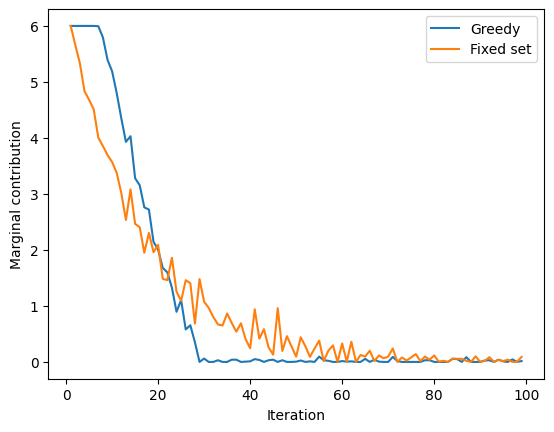
\includegraphics[width=\linewidth,height=0.78\textheight,keepaspectratio]{arxiv2604-24884v1-image-02.png}\par

Figure 2: The computation is carried out for $n=m=100,d=6$ and the marginal contributions of Greedy and the fixed set are calculated by averaging over $200$ runs.





\par\medskip\noindent\textbf{C.2 Analysis For The Different Regions}\par




See 5\par




\par\medskip\noindent\textbf{Proof.}\par



To upper bound the optimal solution, first notice that $|N(\mathcal{O}_{k})|=\max_{S\in\binom{L}{k}}|N(S)|$.
Let $\delta=\sqrt{\frac{24}{\epsilon}\left(\frac{1}{\epsilon d}+\frac{\max(0,\log{\epsilon d})}{\epsilon d}+\frac{\log{n}}{n}\right)}$ and we show that $\delta\in(0,1)$:\par


\[\begin{gathered}
\displaystyle\delta=\sqrt{\frac{24}{\epsilon}\left(\frac{1}{\epsilon d}+\frac{\max(0,\log{\epsilon d})}{\epsilon d}+\frac{\log{n}}{n}\right)}\leq\sqrt{\frac{24}{\epsilon}\left(\frac{1}{\epsilon d}+\frac{1}{\sqrt{\epsilon d}}+\frac{1}{\sqrt{n}}\right)}\leq\sqrt{\frac{24}{\epsilon}\cdot\frac{3}{\epsilon\sqrt{d}}}=\frac{\sqrt{72}}{\epsilon d^{1/4}}\leq\frac{\epsilon}{2},
\end{gathered}\]


where the first inequality is due to $\frac{\max(0,\log{x})}{x}\leq\frac{1}{\sqrt{x}}$ for all $x$, the second inequality is due to $d\geq\sqrt{d},\sqrt{\epsilon}\geq\epsilon$ and $n\geq d\geq\epsilon^{2}d$ and the third inequality is by assumption $d\geq\frac{20^{4}}{\epsilon^{8}}$.
By union bound over $S\in\binom{L}{k}$ and Chernoff bound:\par


\[\begin{gathered}
\displaystyle\Pr\left[|N(\mathcal{O}_{k})|\geq(1+\delta)\cdot\E\left[|N(H_{k})|\right]\right] \displaystyle=\Pr\left[\max_{S\in\binom{L}{k}}|N(S)|\geq(1+\delta)\cdot\E\left[|N(H_{k})|\right]\right] \\
\displaystyle\leq\sum_{S\in\binom{L}{k}}\Pr\left[|N(S)|\geq(1+\delta)\cdot\E\left[|N(H_{k})|\right]\right] \\
\displaystyle\leq\sum_{S\in\binom{L}{k}}\Pr\left[|N(S)|\geq(1+\delta)\cdot\E\left[|N(S)|\right]\right] \\
\displaystyle\leq\sum_{S\in\binom{L}{k}}\exp\left(-\frac{\delta^{2}}{3}\cdot\E\left[|N(S)|\right]\right) \\
\displaystyle=\sum_{S\in\binom{L}{k}}\exp\left(-\frac{\delta^{2}}{3}\cdot\E\left[|N(H_{k})|\right]\right) \\
\displaystyle=\exp\left(\log{\binom{n}{k}}-\frac{\delta^{2}}{3}\E\left[|N(H_{k})|\right]\right),
\end{gathered}\]


where the first line is by definition of $\mathcal{O}_{k}$, the second line is by union bound, the third line is because $\E\left[|N(S)|\right]=\E\left[|N(H_{k})|\right]$ for all $S\in\binom{L}{k}$, the fourth line is by Lemma 33 since $\delta\in(0,1)$ by Equation (1), the fifth line is because $\E\left[|N(S)|\right]=\E\left[|N(H_{k})|\right]$ and the sixth line is because $|\binom{L}{k}|=\binom{n}{k}=e^{\log{\binom{n}{k}}}$.
We upper bound the exponent as follows:\par


\[\begin{gathered}
\displaystyle\log{\binom{n}{k}}-\frac{\delta^{2}}{3}\E\left[|N(H_{k})|\right] \displaystyle\leq k\log\left(\frac{en}{k}\right)-8\left(\frac{1+\max(0,\log{\epsilon d})}{\epsilon^{2}d}+\frac{\log{n}}{\epsilon n}\right)\cdot\left(1-e^{-kd/n}\right)\cdot n \\
\displaystyle\leq\frac{1+\log{\frac{\epsilon d}{2}}}{\frac{\epsilon d}{2}}\cdot n-8\left(\frac{1+\max(0,\log{\epsilon d})}{\epsilon^{2}d}+\frac{\log{n}}{\epsilon n}\right)\cdot\left(1-e^{-\epsilon/2}\right)\cdot n \\
\displaystyle\leq\frac{1+\log{\frac{\epsilon d}{2}}}{\frac{\epsilon d}{2}}\cdot n-8\left(\frac{1+\max(0,\log{\epsilon d})}{\epsilon^{2}d}+\frac{\log{n}}{\epsilon n}\right)\cdot\frac{\epsilon}{4}\cdot n \\
\displaystyle\leq\frac{1+\max(0,\log{\epsilon d})}{\frac{\epsilon d}{2}}\cdot n-\left(\frac{1+\max(0,\log{\epsilon d})}{\frac{\epsilon d}{2}}+\frac{2\log{n}}{n}\right)\cdot n \\
\displaystyle=-2\log{n} \\
\displaystyle\leq-\log{n},
\end{gathered}\]


where the first line is due to $\binom{n}{k}\leq\left(\frac{en}{k}\right)^{k}$ and Lemma 4, the second line is because $k\log\left(\frac{en}{k}\right)$ is increasing for all $k\in[n]$ and $\frac{\epsilon n}{2d}\leq k\leq\frac{2n}{\epsilon d}$ by assumption, the third line is because $1-e^{-\epsilon}\geq\frac{\epsilon}{2}$ for all $\epsilon\in(0,1)$ and the fourth line is due to $\epsilon d\geq\frac{\epsilon d}{2}$.
Let event $F=\{|N(\mathcal{O}_{k})|\geq(1+\delta)\cdot\E\left[|N(H_{k})|\right]\}$.
We are ready to upper bound the expected value of Opt:\par


\[\begin{gathered}
\displaystyle\E\left[|N(\mathcal{O}_{k})|\right] \displaystyle=\E\left[|N(\mathcal{O}_{k})|\middle|F\right]\cdot\Pr\left[F\right]+\E\left[|N(\mathcal{O}_{k})|\middle|\bar{F}\right]\cdot\Pr\left[\bar{F}\right] \\
\displaystyle\leq n\cdot\frac{1}{n}+\E\left[|N(\mathcal{O}_{k})|\middle|\bar{F}\right]\cdot 1 \\
\displaystyle\leq 1+(1+\delta)\cdot\E\left[|N(H_{k})|\right] \\
\displaystyle\leq\left(1+\delta+\frac{\epsilon}{2}\right)\cdot\E\left[|N(H_{k})|\right] \\
\displaystyle\leq\left(1+\epsilon\right)\cdot\E\left[|N(H_{k})|\right] \\
\displaystyle\leq\left(1+\epsilon\right)\cdot\E\left[|N(\mathcal{G}_{k})|\right],
\end{gathered}\]


where the first line is by tower rule, the second line is because $|N(\mathcal{O}_{k})|\leq n$ and $\Pr\left[F\right]\leq\exp\left(-\log{n}\right)=\frac{1}{n}$ by substituting Equation (2a) to (2), the third line follows by definition of $F$, the fourth line is because $1=\frac{\E\left[|N(H_{k})|\right]}{\E\left[|N(H_{k})|\right]}\leq\frac{\E\left[|N(H_{k})|\right]}{\left(1-e^{-\epsilon/2}\right)\cdot n}\leq\frac{\E\left[|N(H_{k})|\right]}{\frac{\epsilon}{4}\cdot n}\leq\frac{\epsilon}{2}\cdot\E\left[|N(H_{k})|\right]$ by assumption $n\geq d\geq\frac{20^{4}}{\epsilon^{8}}$, the fifth line is because $\delta\leq\frac{\epsilon}{2}$ by Equation (1) and the sixth line is by Lemma 2.
The statement follows directly from Equation (3):\par


\[\begin{gathered}
\displaystyle\E\left[|N(\mathcal{G}_{k})|\right]\geq\frac{1}{1+\epsilon}\cdot\E\left[|N(\mathcal{O}_{k})|\right]\geq\left(1-\epsilon\right)\cdot\E\left[|N(\mathcal{O}_{k})|\right].
\end{gathered}\]


where the second inequality is because $\frac{1}{1+\epsilon}\geq 1-\epsilon$.
\ensuremath{\blacksquare}\par





See 6\par




\par\medskip\noindent\textbf{Proof.}\par



Let $t^{*}_{d}=\left(1-\left(1+d(d-1)\right)^{-\frac{1}{d-1}}\right)\cdot\frac{n}{d}$ and $\delta=3e^{d^{2}}\cdot\sqrt{8n\log{2n}}$.
Then:\par


\[\begin{gathered}
\displaystyle\Pr\left[|t_{d}-t^{*}_{d}|\leq\delta\right]\geq 1-\frac{1}{n},
\end{gathered}\]


which follows by Lemma 1 as $n\geq 2d^{2}$ by assumption.
For $k\leq t^{*}_{d}-\delta$, Greedy gains $d$ on each iteration so:\par


\[\begin{gathered}
\displaystyle\E\left[|N(\mathcal{G}_{k})|\right]\geq\Pr\left[|t_{d}-t^{*}_{d}|\leq\delta\right]\cdot\E\left[|N(\mathcal{G}_{k})|\middle||t_{d}-t^{*}_{d}|\leq\delta\right]\geq\left(1-\frac{1}{n}\right)\cdot kd\geq\left(1-\frac{1}{n}\right)\cdot\E\left[|N(\mathcal{O}_{k})|\right],
\end{gathered}\]


where the second inequality is due to Equation (1).
For $k\geq t^{*}_{d}-\delta$, Greedy gains $d$ on each iteration until $t^{*}_{d}-\delta$ and after that we use the worst case analysis which gives:\par


\[\begin{gathered}
\displaystyle\E\left[|N(\mathcal{G}_{k})|\right] \displaystyle\geq\Pr\left[|t_{d}-t^{*}_{d}|\leq\delta\right]\cdot\E\left[|N(\mathcal{G}_{k})\middle||t_{d}-t^{*}_{d}|\leq\delta\right] \\
\displaystyle\geq\left(1-\frac{1}{n}\right)\cdot\E\left[|N(\mathcal{G}_{k})|\middle||t_{d}-t^{*}_{d}|\leq\delta\right] \\
\displaystyle\geq\left(1-\frac{1}{n}\right)\cdot\left(1-\frac{1}{e}+\frac{1}{e}\cdot\left(\frac{t^{*}_{d}-\delta}{n/d}\right)^{3}\right)\cdot\E\left[|N(\mathcal{O}_{k})|\middle||t_{d}-t^{*}_{d}|\leq\delta\right],
\end{gathered}\]


where the first line is by tower rule, the second line is due to Equation (1), the third line is due to Lemma 7 since $k\geq t^{*}_{d}-\delta\geq t_{d}$ by the condition.
For the conditional value of Opt we have:\par


\[\begin{gathered}
\displaystyle\E \displaystyle\left[|N(\mathcal{O}_{k})|\right]= \\
\displaystyle=\E\left[|N(\mathcal{O}_{k})|\middle||t_{d}-t^{*}_{d}|\leq\delta\right]\cdot\Pr\left[|t_{d}-t^{*}_{d}|\leq\delta\right]+\E\left[|N(\mathcal{O}_{k})|\middle||t_{d}-t^{*}_{d}|>\delta\right]\cdot\Pr\left[|t_{d}-t^{*}_{d}|>\delta\right] \\
\displaystyle\leq\E\left[|N(\mathcal{O}_{k})|\middle||t_{d}-t^{*}_{d}|\leq\delta\right]\cdot 1+n\cdot\frac{1}{n} \\
\displaystyle=\E\left[|N(\mathcal{O}_{k})|\middle||t_{d}-t^{*}_{d}|\leq\delta\right]+1 \\
\displaystyle\Rightarrow\E\left[|N(\mathcal{O}_{k})|\middle||t_{d}-t^{*}_{d}|\leq\delta\right]\geq\E\left[|N(\mathcal{O}_{k})|\right]-1\geq\left(1-\frac{4}{\epsilon n}\right)\cdot\E\left[|N(\mathcal{O}_{k})|\right],
\end{gathered}\]


where the first line is by tower rule, the second line is due to $|N(\mathcal{O}_{k})|\leq n$ and Equation (1), the third line is by cancellation and the fourth line is because $1\leq\frac{\E\left[|N(\mathcal{O}_{k})|\right]}{\E\left[|N(H_{k})|\right]}\leq\frac{\E\left[|N(\mathcal{O}_{k})|\right]}{\left(1-e^{-\epsilon/2}\right)\cdot n}\leq\frac{4}{\epsilon n}\cdot\E\left[|N(\mathcal{O}_{k})|\right]$ by Lemma 4.
Substituting Equation (3a) to (3) we have:\par


\[\begin{gathered}
\displaystyle\E\left[|N(\mathcal{G}_{k})|\right] \displaystyle\geq\left(1-\frac{1}{n}\right)\cdot\left(1-\frac{1}{e}+\frac{1}{e}\cdot\left(\frac{t^{*}_{d}-\delta}{n/d}\right)^{3}\right)\cdot\left(1-\frac{4}{\epsilon n}\right)\cdot\E\left[|N(\mathcal{O}_{k})|\right] \\
\displaystyle\geq\left(1-\frac{1}{e}+\frac{1}{e}\cdot\left(\frac{t^{*}_{d}-\delta}{n/d}\right)^{3}-\frac{8}{\epsilon n}\right)\cdot\E\left[|N(\mathcal{O}_{k})|\right],
\end{gathered}\]


where the second line is because $\frac{1}{n}\leq\frac{4}{\epsilon n}$.
At this point it suffices to show that $\frac{t^{*}_{d}-\delta}{n/d}$ is lower bounded by a positive constant:\par


\[\begin{gathered}
\displaystyle\frac{t^{*}_{d}-\delta}{n/d}\geq\frac{1}{d}-\frac{3e^{d^{2}}\cdot\sqrt{8n\log{2n}}}{n/d}\geq\frac{1}{d}-12de^{d^{2}}\sqrt{\frac{\log{2n}}{2n}}\geq\frac{\epsilon^{8}}{20^{4}}-\frac{\frac{12\cdot 20^{4}}{\epsilon^{8}}e^{\frac{20^{4}}{\epsilon^{8}}}}{(2n)^{1/4}}\geq\frac{\epsilon^{8}}{20^{5}},
\end{gathered}\]


where the first inequality is due to Lemma 38, the second due to $d\leq\frac{8^{4}}{\epsilon^{8}}$, the third is by setting $n_{0}(\epsilon)=8\cdot\left(\frac{12\cdot 20^{8}e^{20^{4}/\epsilon^{8}}}{\epsilon^{16}}\right)^{4}$.
Then we have:\par


\[\begin{gathered}
\displaystyle\E\left[|N(\mathcal{G}_{k})|\right] \displaystyle\geq\left(1-\frac{1}{e}+\frac{1}{e}\cdot\left(\frac{t^{*}_{d}-\delta}{n/d}\right)^{3}-\frac{8}{\epsilon n}\right)\cdot\E\left[|N(\mathcal{O}_{k})|\right] \\
\displaystyle\geq\left(1-\frac{1}{e}+\frac{\epsilon^{24}}{20^{15}e}-\frac{8}{\epsilon n}\right)\cdot\E\left[|N(\mathcal{O}_{k})|\right] \\
\displaystyle\geq\left(1-\frac{1}{e}+\left(\frac{\epsilon}{20}\right)^{24}\right)\cdot\E\left[|N(\mathcal{O}_{k})|\right],
\end{gathered}\]


where the first line is by Equation (4), the second line is by Equation (4a) and the third inequality is due to $n\geq 8\cdot\left(\frac{20}{\epsilon}\right)^{26}$.
By Equation (1) and Equation (5) we obtain the statement.
\ensuremath{\blacksquare}\par





See 7\par




\par\medskip\noindent\textbf{Proof.}\par



For all $k\geq t_{d}$ we have that:\par


\[\begin{gathered}
\displaystyle|N(\mathcal{G}_{k})| \displaystyle\geq\left(1-\exp\left(-\left(1-\frac{t_{d}}{k}\right)\right)\cdot\left(1-\frac{|N(G_{t_{d}})|}{|N(O_{k})|}\right)\right)\cdot|N(O_{k})| \\
\displaystyle\geq\left(1-\exp\left(-\left(1-\frac{t_{d}}{k}\right)\right)\cdot\left(1-\frac{t_{d}\cdot d}{\min\{kd,n\}}\right)\right)\cdot|N(O_{k})| \\
\displaystyle=\left(1-\exp\left(-\left(1-\frac{1}{k/t_{d}}\right)\right)\cdot\left(1-\frac{1}{\min\{k/t_{d},n/t_{d}d\}}\right)\right)\cdot|N(O_{k})| \\
\displaystyle\geq\left(1-\exp\left(-\left(1-\frac{t_{d}}{n/d}\right)\right)\cdot\left(1-\frac{t_{d}}{n/d}\right)\right)\cdot|N(O_{k})| \\
\displaystyle\geq\left(1-\frac{1}{e}+\frac{1}{e}\cdot\left(\frac{t_{d}}{n/d}\right)^{3}\right)\cdot|N(O_{k})|,
\end{gathered}\]


where the first line is due to Lemma 35 for $t=t_{d}$, the second line is because $|N(G_{t_{d}})|=t_{d}\cdot d$ by definition of $t_{d}$ and $|N(O_{k})|\leq\min\{kd,n\}$ for all $k$, the fourth line is by Lemma 36 since $k\geq t_{d}$ and the fifth line is due to Lemma 37 since $t_{d}\leq n/d$ by definition.
\ensuremath{\blacksquare}\par




% SOURCE-ID Thmlemma35


\par\medskip\noindent\textbf{\textbf{Lemma 35}\textbf{.}}\par



\emph{Let $d\in\mathbbm{N}$ and $B=(L,R,E)$ be a bipartite graph.
Then for all $t\leq k$:}\par


\[\begin{gathered}
|N(G_{k})|\geq\left(1-\exp\left(-\left(1-\frac{t}{k}\right)\right)\cdot\left(1-\frac{|N(G_{t})|}{|N(O_{k})|}\right)\right)\cdot|N(O_{k})|.
\end{gathered}\]



% END-SOURCE-ID Thmlemma35



\par\medskip\noindent\textbf{Proof.}\par



We repeat the worst case analysis of Greedy for iterations $k\geq i>t$:\par


\[\begin{gathered}
\displaystyle|N(O_{k})|-|N(G_{k})|\leq\left(1-\frac{1}{k}\right)^{1}\cdot\left(|N(O_{k})|-|N(G_{k-1})|\right)\leq\left(1-\frac{1}{k}\right)^{k-t}\cdot\left(|N(O_{k})|-|N(G_{t})|\right),
\end{gathered}\]


and solving for $|N(G_{k})|$ we have:\par


\[\begin{gathered}
\displaystyle|N(G_{k})| \displaystyle\geq\left(1-\left(1-\frac{1}{k}\right)^{k-t}\cdot\left(1-\frac{|N(G_{t})|}{|N(O_{k})|}\right)\right)\cdot|N(O_{k})| \\
\displaystyle\geq\left(1-\exp\left\{-\left(1-\frac{t}{k}\right)\right\}\cdot\left(1-\frac{|N(G_{t})|}{|N(O_{k})|}\right)\right)\cdot|N(O_{k})|,
\end{gathered}\]


where the first line is by (1) and the second line is due to $1-\frac{1}{k}\leq e^{-\frac{1}{k}}$.
\ensuremath{\blacksquare}\par




% SOURCE-ID Thmlemma36


\par\medskip\noindent\textbf{\textbf{Lemma 36}\textbf{.}}\par



\emph{Let $y\geq 1$ and $f(x)=1-\exp\left(-\left(1-\frac{1}{x}\right)\right)\cdot\left(1-\frac{1}{\min\{x,y\}}\right)$.
Then we have that
$f(x)\geq 1-\exp\left(-\left(1-\frac{1}{y}\right)\right)\cdot\left(1-\frac{1}{y}\right)$ for all $x\geq 1$.}\par



% END-SOURCE-ID Thmlemma36



\par\medskip\noindent\textbf{Proof.}\par



We start with case $x\leq y$:\par


\[\begin{gathered}
\displaystyle f(k)=1-\exp\left(-\left(1-\frac{1}{x}\right)\right)\cdot\left(1-\frac{1}{x}\right)\geq 1-\exp\left(-\left(1-\frac{1}{y}\right)\right)\cdot\left(1-\frac{1}{y}\right).
\end{gathered}\]


For $x>y$:\par


\[\begin{gathered}
\displaystyle f(k)=1-\exp\left(-\left(1-\frac{1}{x}\right)\right)\cdot\left(1-\frac{1}{y}\right)\geq 1-\exp\left(-\left(1-\frac{1}{y}\right)\right)\cdot\left(1-\frac{1}{y}\right).
\end{gathered}\]


\ensuremath{\blacksquare}\par




% SOURCE-ID Thmlemma37


\par\medskip\noindent\textbf{\textbf{Lemma 37}\textbf{.}}\par



\emph{For all $x\leq 1$ we have that $1-e^{-(1-x)}\cdot(1-x)\geq 1-\frac{1}{e}+\frac{x^{3}}{e}$.}\par



% END-SOURCE-ID Thmlemma37



\par\medskip\noindent\textbf{Proof.}\par



We have that:\par


\[\begin{gathered}
\displaystyle 1-e^{-(1-x)}\cdot(1-x) \displaystyle=1-e^{-1}e^{x}\cdot(1-x) \\
\displaystyle\geq 1-e^{-1}(1+x+x^{2})\cdot(1-x) \\
\displaystyle=1-e^{-1}(1-x^{3}) \\
\displaystyle=1-\frac{1}{e}+\frac{x^{3}}{e},
\end{gathered}\]


where the inequality is due to $e^{x}\leq 1+x+x^{2}$ for all $x\leq 1$.
\ensuremath{\blacksquare}\par




% SOURCE-ID Thmlemma38


\par\medskip\noindent\textbf{\textbf{Lemma 38}\textbf{.}}\par



\emph{For all $d\geq 2$ we have that $1-\left(1+d(d-1)\right)^{-\frac{1}{d-1}}\geq\frac{1}{d}$.}\par



% END-SOURCE-ID Thmlemma38



\par\medskip\noindent\textbf{Proof.}\par



Equivalently we show that $\left(1+d(d-1)\right)^{-\frac{1}{d-1}}\leq\frac{d-1}{d}$ or after taking logs:\par


\[\begin{gathered}
\displaystyle\log\left(1+d(d-1)\right)\geq(d-1)\cdot\log\left(\frac{d}{d-1}\right).
\end{gathered}\]


The left-hand side is greater than $1$ since $1+d(d-1)\geq e$ for all $d\geq 2$ and the right-hand side is less than $1$ since $(d-1)\cdot\log\left(\frac{d}{d-1}\right)\leq(d-1)\cdot\frac{1}{d-1}=1$.
\ensuremath{\blacksquare}\par





See 1\par




\par\medskip\noindent\textbf{Proof.}\par



We have:\par


\[\begin{gathered}
\displaystyle\frac{1-e^{-\epsilon}}{\epsilon}\geq\frac{1-(1-\epsilon+\epsilon^{2}))}{\epsilon}=1-\epsilon
\end{gathered}\]


where the inequality is due to $e^{-\epsilon}\leq 1-\epsilon+\epsilon^{2}$ which holds for all $\epsilon\in(0,1)$.
\ensuremath{\blacksquare}\par





See 2\par




\par\medskip\noindent\textbf{Proof.}\par



We have:\par


\[\begin{gathered}
\displaystyle\left(1-\frac{1}{k}\right)^{k}=e^{k\log\left(1-\frac{1}{k}\right)}\leq e^{k\left(-\frac{1}{k}-\frac{1}{2k^{2}}\right)}=e^{-1-\frac{1}{2k}}=e^{-1}\cdot e^{-\frac{1}{2k}}\leq e^{-1}\cdot\left(1-\frac{\frac{1}{2k}}{2}\right)=\frac{1}{e}-\frac{1}{4ek},
\end{gathered}\]


where the first equality is by raising to the exponent, the first inequality is due to inequality $\log\left(1-x\right)\leq-x-\frac{x^{2}}{2}$ for all $x\geq 0$, the second equality is by simplifying the exponent, and the second inequality is due to inequality $e^{-x}\leq 1-\frac{x}{2}$ for all $x\in[0,1]$.
\ensuremath{\blacksquare}\par







\par\medskip\noindent\textbf{Appendix D Omitted Proofs Of Section 4}\par



% SOURCE-ID Thmdefinition4


\par\medskip\noindent\textbf{\textbf{Definition 4}\textbf{ }(Erdos-Renyi random graph)\textbf{.}}\par



$\mathbbm{G}_{n,m}$\emph{ samples graphs $\mathcal{G}=(V,\mathcal{E})$, with $|V|=n$ and $\mathcal{E}\subseteq\binom{V}{2}$ chosen uniformly, such that $|\mathcal{E}|=m$.}\par



% END-SOURCE-ID Thmdefinition4


% SOURCE-ID Thmdefinition5


\par\medskip\noindent\textbf{\textbf{Definition 5}\textbf{ }(Random graph with replacement)\textbf{.}}\par



$\mathbbm{G}^{r}_{n,m}$\emph{ samples graphs $\mathcal{G}^{r}=(V,\mathcal{E}^{r})$, with $|V|=n$. Also let $e_{1},e_{2},\dots,e_{m}\in\binom{V}{2}$ be independent uniform random samples (with replacement), then $\mathcal{E}^{r}=\{e_{1},\dots,e_{m}\}$.}\par



% END-SOURCE-ID Thmdefinition5


% SOURCE-ID Thmdefinition6


\par\medskip\noindent\textbf{\textbf{Definition 6}\textbf{ }(Maximum matching)\textbf{.}}\par



\emph{Let $G=(V,E)$ and let $M$ be a maximum matching on $G$. We denote the size of this matching as $\mu(G)=|M|$ .}\par



% END-SOURCE-ID Thmdefinition6


% SOURCE-ID Thmdefinition7


\par\medskip\noindent\textbf{\textbf{Definition 7}\textbf{ }(Maximum matching on random graphs)\textbf{.}}\par



\emph{Let $\mathcal{G}\sim\mathbbm{G}_{n,m}$ and $\mathcal{G}^{r}\sim\mathbbm{G}^{r}_{n,m}$.
Then $\mu(n,m)=\mu(\mathcal{G})$ denotes the size of the maximum matching on $\mathcal{G}$ and $\mu^{r}(n,m)=\mu(\mathcal{G}^{r})$ denotes the size of the maximum matching on $\mathcal{G}^{r}$.}\par



% END-SOURCE-ID Thmdefinition7



We state a classic result for the size of maximum matchings in random graphs by [16], but we use the statement of [3]. The difference in some constants is because we assume $n=cm$, while in the original matching setting it was $n=cm/2$.\par



% SOURCE-ID Thmlemma39


\par\medskip\noindent\textbf{\textbf{Lemma 39}\textbf{.}}\par



{\itshape [Theorem 4 in [3]]

Let $n=cm$ for some constant $c>0$ and sample graph $\mathcal{G}$ from $\mathbbm{G}_{m,n}$.
Then for any constant $\epsilon>0$ we have that:}\par


\[\begin{gathered}
\displaystyle\Pr\left[\middle|\frac{\mu(m,n)}{m}-\left(1-\frac{\gamma^{*}+\gamma_{*}+\gamma^{*}\gamma_{*}}{4c}\right)\middle|\geq m^{-\frac{1}{7}+\epsilon}\right]=o(1),
\end{gathered}\]


\emph{where $\gamma_{*}$ is the smallest root of $x=2ce^{-2ce^{-x}}$ and $\gamma^{*}=2ce^{-\gamma_{*}}$.}\par



% END-SOURCE-ID Thmlemma39



The following lemma shows that with high probability there is a sublinear number of pairs of duplicated edges in graphs drawn from model $\mathbbm{G}^{r}_{n,n}$.\par



% SOURCE-ID Thmlemma40


\par\medskip\noindent\textbf{\textbf{Lemma 40}\textbf{.}}\par



\emph{Draw $\mathcal{G}^{r}(V,\mathcal{E}^{r})\sim\mathbbm{G}^{r}_{n,n}$.
Then $\Pr\left[n-|\mathcal{E}^{r}|\geq\log{n}\right]\leq\frac{1}{\log{n}}$.}\par



% END-SOURCE-ID Thmlemma40



\par\medskip\noindent\textbf{Proof.}\par



Let $X=n-|\mathcal{E}^{r}|$, then $X\leq\sum_{1\leq i<j\leq n}\mathbbm{1}\{e_{i}=e_{j}\}$, since the right-hand side counts more collisions when the same edge is sampled multiple times.
Let $i\neq j$ arbitrary and we have that:\par


\[\begin{gathered}
\displaystyle\Pr\left[e_{i}=e_{j}\right] \displaystyle=\sum_{\{v,v^{\prime}\}\in\binom{V}{2}}\Pr\left[e_{i}=\{v,v^{\prime}\},e_{j}=\{v,v^{\prime}\}\right] \\
\displaystyle=\sum_{\{v,v^{\prime}\}\in\binom{V}{2}}\Pr\left[e_{i}=\{v,v^{\prime}\}\right]\cdot\Pr\left[e_{j}=\{v,v^{\prime}\}\right] \\
\displaystyle=\binom{n}{2}\cdot\left(\frac{1}{\binom{n}{2}}\right)^{2} \\
\displaystyle=\frac{1}{\binom{n}{2}},
\end{gathered}\]


where the first line is by law of total probability, the second line is due to independent choice of edges and the third line is because edges are chosen uniformly at random with replacement.
For the expectation of $X$ we have that:\par


\[\begin{gathered}
\displaystyle\E[X]\leq\sum_{1\leq i<j\leq n}\Pr\left[e_{i}=e_{j}\right]=\sum_{1\leq i<j\leq n}\frac{1}{\binom{n}{2}}=\frac{\binom{n}{2}}{\binom{n}{2}}=1
\end{gathered}\]


where the second equality is by (1).
Finally we show the statement:\par


\[\begin{gathered}
\displaystyle\Pr\left[X\geq\log{n}\right]\leq\frac{\E[X]}{\log{n}}\leq\frac{1}{\log{n}},
\end{gathered}\]


where the first inequality is by Markov and the second is due to (2).
\ensuremath{\blacksquare}\par





Now we show that the maximum matching size in both random graph models is close.\par



% SOURCE-ID Thmlemma41


\par\medskip\noindent\textbf{\textbf{Lemma 41}\textbf{.}}\par



$\Pr\left[\mu^{r}(n,n)\geq x\right]\geq\Pr\left[\mu(n,n)\geq x+\log{n}\right]\cdot\left(1-\frac{1}{\log{n}}\right)$\emph{ for all $x$.}\par



% END-SOURCE-ID Thmlemma41



\par\medskip\noindent\textbf{Proof.}\par



We construct a coupling between $\mathbbm{G}^{r}_{n,n}$ and $\mathbbm{G}_{n,n}$ by first sampling $\hat{\mathcal{G}}^{r}=(V,\hat{\mathcal{E}}^{r})\sim\mathbbm{G}^{r}_{n,n}$ and then sampling an additional $n-|\hat{\mathcal{E}}^{r}|$ edges from $\binom{V}{2}\setminus\hat{\mathcal{E}}^{r}$ without replacement to obtain $\hat{\mathcal{G}}_{n,n}=(V,\hat{\mathcal{E}})\sim\mathbbm{G}_{n,n}$.
Then we have that:\par


\[\begin{gathered}
\displaystyle\Pr\left[\mu^{r}(n,n)\geq x\right] \displaystyle=\Pr\left[\mu(\hat{\mathcal{G}^{r}})\geq x\right] \\
\displaystyle\geq\Pr\left[\mu(\hat{\mathcal{G}^{r}})\geq x\middle||\hat{\mathcal{E}}\setminus\hat{\mathcal{E}}^{r}|\leq\log{n}\right]\cdot\Pr\left[|\hat{\mathcal{E}}\setminus\hat{\mathcal{E}}^{r}|\leq\log{n}\right] \\
\displaystyle\geq\Pr\left[\mu(\hat{\mathcal{G}^{r}})\geq x\middle||\hat{\mathcal{E}}\setminus\hat{\mathcal{E}}^{r}|\leq\log{n}\right]\cdot\left(1-\frac{1}{\log{n}}\right) \\
\displaystyle\geq\Pr\left[\mu(\hat{\mathcal{G}})\geq x+\log{n}\middle||\hat{\mathcal{E}}\setminus\hat{\mathcal{E}}^{r}|\leq\log{n}\right]\cdot\left(1-\frac{1}{\log{n}}\right) \\
\displaystyle=\Pr\left[\mu(\hat{\mathcal{G}})\geq x+\log{n}\right]\cdot\left(1-\frac{1}{\log{n}}\right) \\
\displaystyle=\Pr\left[\mu(n,n)\geq x+\log{n}\right]\cdot\left(1-\frac{1}{\log{n}}\right),
\end{gathered}\]


where the first line is by definition of $\hat{\mathcal{G}}^{r}$, the second line is by law of total probability, the third line is by Lemma 40 since $|\hat{\mathcal{E}}\setminus\hat{\mathcal{E}}^{r}|=n-|\hat{\mathcal{E}}^{r}|$, the fourth line is because conditional on $|\hat{\mathcal{E}}\setminus\hat{\mathcal{E}}^{r}|\leq\log{n}$ we have $\mu(\hat{\mathcal{G}}^{r})\geq\mu(\hat{\mathcal{G}})-\log{n}$, so $\mu(\hat{\mathcal{G}})\geq x+\log{n}$ implies $\mu(\hat{\mathcal{G}^{r}})\geq x$, the fifth line is due to the condition being independent of matching size $\mu(\hat{\mathcal{G}})$ and the sixth line by definition of $\hat{\mathcal{G}}$.
\ensuremath{\blacksquare}\par





The following lemma gives a bound for the size of the maximum matching in graphs sampled from $\mathbbm{G}^{r}_{n,n}$, with high probability. It is only slightly weaker than Lemma 39, which is the corresponding result for Erdős-Renyi $\mathbbm{G}_{n,n}$.
See 10\par




\par\medskip\noindent\textbf{Proof.}\par



Then we have that:\par


\[\begin{gathered}
\displaystyle\Pr \displaystyle\left[\mu(\mathcal{I}_{\mathcal{B}})\geq\left(1-\frac{\gamma^{*}+\gamma_{*}+\gamma^{*}\gamma_{*}}{4}-n^{-\frac{1}{9}}\right)\cdot n\right]= \\
\displaystyle=\Pr\left[\mu^{r}(n,n)\geq\left(1-\frac{\gamma^{*}+\gamma_{*}+\gamma^{*}\gamma_{*}}{4}-n^{-\frac{1}{9}}\right)\cdot n\right] \\
\displaystyle\geq\Pr\left[\mu(n,n)\geq\left(1-\frac{\gamma^{*}+\gamma_{*}+\gamma^{*}\gamma_{*}}{4}-n^{-\frac{1}{9}}\right)\cdot n+\log{n}\right]\cdot\left(1-\frac{1}{\log{n}}\right) \\
\displaystyle=\Pr\left[\mu(n,n)-\left(1-\frac{\gamma^{*}+\gamma_{*}+\gamma^{*}\gamma_{*}}{4}\right)n\geq\log{n}-n^{1-\frac{1}{9}}\right]\cdot\left(1-\frac{1}{\log{n}}\right) \\
\displaystyle\geq\Pr\left[\mu(n,n)-\left(1-\frac{\gamma^{*}+\gamma_{*}+\gamma^{*}\gamma_{*}}{4}\right)n\geq-n^{1-\frac{1}{8}}\right]\cdot\left(1-\frac{1}{\log{n}}\right) \\
\displaystyle\geq\Pr\left[\big|\mu(n,n)-\left(1-\frac{\gamma^{*}+\gamma_{*}+\gamma^{*}\gamma_{*}}{4}\right)n\big|\leq n^{1-\frac{1}{8}}\right]\cdot\left(1-\frac{1}{\log{n}}\right) \\
\displaystyle=1-\Pr\left[\big|\frac{\mu(n,n)}{n}-\left(1-\frac{\gamma^{*}+\gamma_{*}+\gamma^{*}\gamma_{*}}{4}\right)\big|\geq n^{-\frac{1}{8}}\right]\cdot\left(1-\frac{1}{\log{n}}\right) \\
\displaystyle=1-o(1),
\end{gathered}\]


the first line is by definition of $\mu^{r}(n,n)$, the second line is due to Lemma 41, the fourth line is due to $\log{n}-n^{1-1/9}=\log{n}-n^{8/9}\leq-n^{7/8}=-n^{1-1/8}$ by the assumption for large $n$, the fifth line is because this event is a subset, the sixth line is by taking the complement and the seventh line is due to Lemma 39 for $\epsilon=\frac{1}{7}-\frac{1}{8}>0$.
\ensuremath{\blacksquare}\par






\par\medskip\noindent\textbf{Appendix E Generalization to Unbalanced Bipartite Graphs}\par




In this section we generalize Theorem 1 to the case $n=O(m)$. We assume $n=c\cdot m$ and we show a lower bound for the ratio that decreases as $c$ increases. Nevertheless, for all constant $c$, we obtain a bound that is a constant away from $1-\frac{1}{e}$.
Our analysis is very similar to that of Theorem 1, except for the case where the number of left nodes is much smaller than the number of right nodes, i.e. $c$ much smaller than $1$.
We use random model ULRR, which we define as follows.\par



% SOURCE-ID Thmdefinition8


\par\medskip\noindent\textbf{\textbf{Definition 8}\textbf{.}}\par



\emph{Let $n,m\in\mathbbm{N}$ and $d\in[m]$. The random model ULRR($n,m,d$) samples bipartite graphs $\mathcal{B}=(L,R,\mathcal{E})$ from GenR($n,m,d$).}\par



% END-SOURCE-ID Thmdefinition8



In this section we use results from Appendix B, which hold since GenR is a generalization.\par




\par\medskip\noindent\textbf{E.1 Linear And Saturated Regions.}\par



% SOURCE-ID Thmlemma42


\par\medskip\noindent\textbf{\textbf{Lemma 42}\textbf{.}}\par



\emph{Let $\epsilon\in(0,1)$, $m\in\mathbbm{N}$, $c\geq 0$, $n=cm$, $d\in[m],k\in\left[0,\frac{\epsilon m}{2d}\right]\cup\left[\frac{2m}{\epsilon d},n\right]$ and $\mathcal{B}\sim\textsc{ULRR}(n,m,d)$.
Then we have $\E\left[|N(\mathcal{G}_{k})|\right]\geq\left(1-\epsilon\right)\cdot\E\left[|N(\mathcal{O}_{k})|\right]$.}\par



% END-SOURCE-ID Thmlemma42



\par\medskip\noindent\textbf{Proof.}\par



For $k\leq\frac{\epsilon m}{2d}$ we have that:\par


\[\begin{gathered}
\displaystyle\E\left[|N(\mathcal{G}_{k})|\right] \displaystyle\geq\E\left[|N(H_{k})|\right] \\
\displaystyle\geq\left(1-e^{-kd/m}\right)\cdot m \\
\displaystyle=\frac{1-e^{-kd/m}}{kd/m}\cdot kd \\
\displaystyle\geq\frac{1-e^{-\epsilon}}{\epsilon}\cdot kd \\
\displaystyle\geq\left(1-\epsilon\right)\cdot kd \\
\displaystyle\geq\left(1-\epsilon\right)\cdot\E\left[|N(\mathcal{O}_{k})|\right],
\end{gathered}\]


where the first line is by Lemma 18, the second line is by Lemma 17, the fourth line is due to assumption $k\leq\frac{\epsilon m}{2d}\leq\frac{\epsilon m}{d}$, the fifth line is because $\frac{1-e^{-\epsilon}}{\epsilon}\geq(1-\epsilon)$ and the sixth line is due to $kd\geq|N(\mathcal{O}_{k})|$ by Lemma 30.
For $k\geq\frac{2m}{\epsilon d}$ we have that:\par


\[\begin{gathered}
\displaystyle\E\left[|N(\mathcal{G}_{k})|\right] \displaystyle\geq\E\left[|N(H_{k})|\right] \\
\displaystyle\geq\left(1-e^{-kd/m}\right)\cdot m \\
\displaystyle\geq\left(1-e^{-\frac{1}{\epsilon}}\right)\cdot m \\
\displaystyle\geq\left(1-\epsilon\right)\cdot m \\
\displaystyle\geq\left(1-\epsilon\right)\cdot\E\left[|N(\mathcal{O}_{k})|\right],
\end{gathered}\]


where the first line is due to Lemma 18, the second line is due to Lemma 17, the third is by assumption $k\geq\frac{2m}{\epsilon d}\geq\frac{m}{\epsilon d}$, the fourth line is due to $1-e^{-\frac{1}{\epsilon}}\geq 1-\frac{1}{1/\epsilon}=1-\epsilon$ for all $\epsilon\in(0,1)$ and the fifth line is due to $m\geq|N(\mathcal{O}_{k})|$ by Lemma 30.
By (1) and (2) we obtain the statement.
\ensuremath{\blacksquare}\par






\par\medskip\noindent\textbf{E.2 Critical Region: Large Degrees.}\par



% SOURCE-ID Thmlemma43


\par\medskip\noindent\textbf{\textbf{Lemma 43}\textbf{.}}\par



\emph{Let $\epsilon\in(0,1)$, $m\in\mathbbm{N}$, $c\geq 0$, $n=cm$, $d\geq\frac{20^{4}\max(1,c^{2})}{\epsilon^{8}},k\in[\frac{\epsilon m}{2d},\frac{2m}{\epsilon d}]$ and $\mathcal{B}\sim\textsc{ULRR}(n,m,d)$.
Then we have $\E\left[|N(\mathcal{G}_{k})|\right]\geq\left(1-\epsilon\right)\cdot\E[|N(\mathcal{O}_{k})|]$.}\par



% END-SOURCE-ID Thmlemma43



\par\medskip\noindent\textbf{Proof.}\par



To upper bound the optimal solution, first notice that $|N(\mathcal{O}_{k})|=\max_{S\in\binom{L}{k}}|N(S)|$.
Also let\par


\[\begin{gathered}
\delta=\sqrt{\frac{24}{\epsilon}\left(\max\left(0,\frac{\log{ec}+\log{\frac{\epsilon d}{2}}}{\epsilon d}\right)+\frac{\log{m}}{m}\right)}.
\end{gathered}\]


We proceed to show that $\delta\in(0,1)$:\par


\[\begin{gathered}
\displaystyle\delta \displaystyle\leq\sqrt{\frac{24}{\epsilon}\left(\max\left(0,\frac{\log{ec}}{\sqrt{d}}\cdot\frac{1}{\epsilon\sqrt{d}}+\frac{\log{\epsilon d}}{\epsilon d}\right)+\frac{\log{m}}{m}\right)} \\
\displaystyle\leq\sqrt{\frac{24}{\epsilon}\left(\max\left(0,\frac{1}{\epsilon\sqrt{d}}+\frac{1}{\sqrt{\epsilon d}}\right)+\frac{1}{\sqrt{m}}\right)} \\
\displaystyle\leq\frac{\sqrt{72}}{\epsilon d^{1/4}} \\
\displaystyle\leq\frac{\epsilon}{2},
\end{gathered}\]


where the second line is due to $d\geq\frac{20^{4}\max(1,c^{2})}{\epsilon^{8}}\geq(\max(1,\log{ec}))^{2}$ and $\frac{\log{x}}{x}\leq\frac{1}{\sqrt{x}}$ for all $x$, the third line is due to $\sqrt{\epsilon}\geq\epsilon,m\geq d\geq\epsilon^{2}d$ and the fourth line is by assumption $d\geq\frac{20^{4}}{\epsilon^{8}}$.
Then we have:\par


\[\begin{gathered}
\displaystyle\Pr\left[|N(\mathcal{O}_{k})|\geq(1+\delta)\cdot\E\left[|N(H_{k})|\right]\right] \displaystyle=\Pr\left[\max_{S\in\binom{L}{k}}|N(S)|\geq(1+\delta)\cdot\E\left[|N(H_{k})|\right]\right] \\
\displaystyle\leq\sum_{S\in\binom{L}{k}}\Pr\left[|N(S)|\geq(1+\delta)\cdot\E\left[|N(H_{k})|\right]\right] \\
\displaystyle\leq\sum_{S\in\binom{L}{k}}\Pr\left[|N(H_{k})|\geq(1+\delta)\cdot\E\left[|N(H_{k})|\right]\right] \\
\displaystyle\leq\sum_{S\in\binom{L}{k}}\exp\left(-\frac{\delta^{2}}{3}\cdot\E\left[|N(H_{k})|\right]\right) \\
\displaystyle=\exp\left(\log{\binom{n}{k}}-\frac{\delta^{2}}{3}\E\left[|N(H_{k})|\right]\right),
\end{gathered}\]


where the first line is by definition of $\mathcal{O}_{k}$, the second line is by union bound, the third line is because $|N(S)|$ is dominated by $|N(H_{k})$ for all $S\in\binom{L}{k}$ by Lemma 24, the fourth line is by Lemma 33 since $\delta\in(0,1)$ by Equation (1) and the fifth line is because $|\binom{L}{k}|=\binom{n}{k}=e^{\log{\binom{n}{k}}}$.
We upper bound the exponent as follows:\par


\[\begin{gathered}
\displaystyle\log{\binom{n}{k}}-\frac{\delta^{2}}{3}\E\left[|N(H_{k})|\right] \displaystyle\leq k\log\left(\frac{en}{k}\right)-\frac{\delta^{2}}{3}\cdot\left(1-e^{-kd/m}\right)\cdot m \\
\displaystyle\leq\frac{\log{\frac{ec\epsilon d}{2}}}{\frac{\epsilon d}{2}}\cdot m-\frac{\delta^{2}}{3}\cdot\left(1-e^{-\epsilon/2}\right)\cdot m \\
\displaystyle\leq\frac{\log{ec}+\log{\frac{\epsilon d}{2}}}{\frac{\epsilon d}{2}}\cdot m-\frac{\delta^{2}}{3}\cdot\frac{\epsilon}{4}\cdot m \\
\displaystyle\leq\frac{\log{ec}+\log{\frac{\epsilon d}{2}}}{\frac{\epsilon d}{2}}\cdot m-\left(\frac{\log{ec}+\log{\frac{\epsilon d}{2}}}{\frac{\epsilon d}{2}}+\frac{2\log{m}}{m}\right)\cdot m \\
\displaystyle\leq-\log{m},
\end{gathered}\]


where the first line is due to $\binom{n}{k}\leq\left(\frac{en}{k}\right)^{k}$ and Lemma 17, the second line is because $k\log\left(\frac{en}{k}\right)$ is increasing for all $k\in[n]$ and $\frac{\epsilon m}{2d}\leq k\leq\frac{2m}{\epsilon d}$ by assumption, the third line is because $1-e^{-\epsilon/2}\geq\frac{\epsilon}{4}$ for all $\epsilon\in(0,1)$, the fourth line is by definition of $\delta$ and the fifth line is due to $-2\log{m}\leq-\log{m}$.
Let event $F=\{|N(\mathcal{O}_{k})|\geq(1+\delta)\cdot\E\left[|N(H_{k})|\right]\}$.
We are ready to upper bound the expected value of Opt:\par


\[\begin{gathered}
\displaystyle\E\left[|N(\mathcal{O}_{k})|\right] \displaystyle=\E\left[|N(\mathcal{O}_{k})|\middle|F\right]\cdot\Pr\left[F\right]+\E\left[|N(\mathcal{O}_{k})|\middle|\bar{F}\right]\cdot\Pr\left[\bar{F}\right] \\
\displaystyle\leq n\cdot\frac{1}{m}+\E\left[|N(\mathcal{O}_{k})|\middle|\bar{F}\right]\cdot 1 \\
\displaystyle\leq c+(1+\delta)\cdot\E\left[|N(H_{k})|\right] \\
\displaystyle\leq\left(1+\delta+\frac{4c}{\epsilon m}\right)\cdot\E\left[|N(H_{k})|\right] \\
\displaystyle\leq\left(1+\epsilon\right)\cdot\E\left[|N(H_{k})|\right] \\
\displaystyle\leq\left(1+\epsilon\right)\cdot\E\left[|N(\mathcal{G}_{k})|\right],
\end{gathered}\]


where the first line is by tower rule, the second line is because $|N(\mathcal{O}_{k})|\leq m$ and $\Pr\left[F\right]\leq\exp\left(-\log{m}\right)=\frac{1}{m}$ by substituting Equation (2a) to (2), the third line follows by definition of $F$, the fourth line is because $c=c\frac{\E\left[|N(H_{k})|\right]}{\E\left[|N(H_{k})|\right]}\leq c\frac{\E\left[|N(H_{k})|\right]}{\left(1-e^{-\epsilon/2}\right)\cdot m}\leq\frac{\E\left[|N(H_{k})|\right]}{\frac{\epsilon}{4c}\cdot m}$, the fifth line is because $\delta\leq\frac{\epsilon}{2}$ by Equation (1) and $m\geq d\geq\frac{20^{4}c^{2}}{\epsilon^{8}}\geq\frac{8c}{\epsilon^{2}}$ and the sixth line is by Lemma 18.
The statement follows directly from Equation (3):\par


\[\begin{gathered}
\displaystyle\E\left[|N(\mathcal{G}_{k})|\right]\geq\frac{1}{1+\epsilon}\cdot\E\left[|N(\mathcal{O}_{k})|\right]\geq\left(1-\epsilon\right)\cdot\E\left[|N(\mathcal{O}_{k})|\right].
\end{gathered}\]


where the second inequality is because $\frac{1}{1+\epsilon}\geq 1-\epsilon$ for all $\epsilon\in(0,1)$.
\ensuremath{\blacksquare}\par






\par\medskip\noindent\textbf{E.3 Critical Region: Small $n$.}\par



% SOURCE-ID Thmlemma44


\par\medskip\noindent\textbf{\textbf{Lemma 44}\textbf{.}}\par



\emph{Let $\epsilon\in(0,1)$, $m\geq\frac{8}{\epsilon^{2}}$, $0\leq c\leq\frac{\epsilon^{3}}{48}-\frac{\log{m}}{m}$, $n=cm$, $d\in[m],k\in[\frac{\epsilon m}{2d},\frac{2m}{\epsilon d}]$ and $\mathcal{B}\sim\textsc{ULRR}(n,m,d)$.
Then we have $\E\left[|N(\mathcal{G}_{k})|\right]\geq\left(1-\epsilon\right)\cdot\E\left[|N(\mathcal{O}_{k})|\right]$.}\par



% END-SOURCE-ID Thmlemma44



\par\medskip\noindent\textbf{Proof.}\par



For $\delta=\frac{\epsilon}{2}\in(0,1)$, by Lemma 28 we have that:\par


\[\begin{gathered}
\displaystyle\E\left[|N(\mathcal{G}_{k})|\right]\geq\left(1-\frac{\epsilon}{2}\right)\cdot\E\left[|N(\mathcal{O}_{k})|\right]-m\cdot\exp\left(\log{\binom{n}{k}}-\frac{\epsilon^{2}}{12}(1-e^{-kd/m})\cdot m\right).
\end{gathered}\]


We upper bound the exponent of the second term:\par


\[\begin{gathered}
\displaystyle\log{\binom{n}{k}}-\frac{\epsilon^{2}}{12}\cdot(1-e^{-kd/m})\cdot m \displaystyle\leq\log{2}\cdot n-\frac{\epsilon^{2}}{12}\cdot(1-e^{-\epsilon/2})\cdot m \\
\displaystyle\leq n-\frac{\epsilon^{3}}{48}\cdot m \\
\displaystyle=\left(c-\frac{\epsilon^{3}}{48}\right)\cdot m \\
\displaystyle\leq-\frac{\log{m}}{m}\cdot m \\
\displaystyle=-\log{m}
\end{gathered}\]


where the first line is due to $\binom{n}{k}\leq 2^{n}$ and $k\geq\frac{\epsilon m}{2d}$ by the assumption, the second line is due to $\log{2}\leq 1$ and $1-e^{-\epsilon/2}\geq\frac{\epsilon}{4}$ for $\epsilon\in(0,1)$, the third line is by assumption $n=cm$ and the fourth line is by assumption $c\leq\frac{\epsilon^{3}}{48}-\frac{\log{m}}{m}$.
Substituting (1a) into (1) we have:\par


\[\begin{gathered}
\displaystyle\E\left[|N(\mathcal{G}_{k})|\right] \displaystyle\geq(1-\frac{\epsilon}{2})\cdot\E\left[|N(\mathcal{O}_{k})|\right]-m\cdot\exp\left(-\log{m}\right) \\
\displaystyle=(1-\frac{\epsilon}{2})\cdot\E\left[|N(\mathcal{O}_{k})|\right]-1 \\
\displaystyle\geq\left(1-\epsilon\right)\cdot\E\left[|N(\mathcal{O}_{k})|\right],
\end{gathered}\]


where the second line is by cancellation and the third line is due to $1\leq\frac{\E\left[|N(\mathcal{O}_{k})|\right]}{\E\left[|N(H_{k})|\right]}\leq\frac{4}{\epsilon m}\cdot\E\left[|N(\mathcal{O}_{k})|\right]$ and $\frac{4}{\epsilon m}\leq\frac{\epsilon}{2}$.
\ensuremath{\blacksquare}\par






\par\medskip\noindent\textbf{E.4 Critical Region: Small Degrees.}\par



% SOURCE-ID Thmlemma45


\par\medskip\noindent\textbf{\textbf{Lemma 45}\textbf{.}}\par



\emph{Let $\epsilon\in(0,1)$, $m\geq\frac{1}{2c}\cdot\left(c\left(\frac{20^{6}c^{2}}{\epsilon^{8}}\right)^{2}e^{\frac{20^{4}c^{3}}{\epsilon^{8}}}\right)^{4}$, $c\geq\frac{\epsilon^{3}}{48}-\frac{\log{m}}{m}$, $n=cm$, $d\leq\frac{20^{4}\max(1,c^{2})}{\epsilon^{8}},k\in[\frac{\epsilon m}{2d},\frac{2m}{\epsilon d}]$ and $\mathcal{B}\sim\textsc{ULRR}(n,m,d)$.
Then there exists a function $f(x,y)$ increasing in $x$ and decreasing in $y$, such that $\E\left[|N(\mathcal{G}_{k})|\right]\geq\left(1-\frac{1}{e}+f(\epsilon,c)\right)\cdot\E[|N(\mathcal{O}_{k})|]$.}\par



% END-SOURCE-ID Thmlemma45



\par\medskip\noindent\textbf{Proof.}\par



Let random variable $t_{d}=\max\{t\in\{1,\dots,n\}:|N(\mathcal{G}_{t})\setminus N(\mathcal{G}_{t-1})|=d\}$.
Notice that by definition, $t_{d}=|\mathcal{A}^{d}_{n}|$, i.e. $t_{d}$ is the number of accepts in the first phase of AcceptReject.
Also let\par


\[\begin{gathered}
\displaystyle t^{*}_{d}=\frac{m}{d}\cdot\left(1-\left(1+cd(d-1)\right)^{-\frac{1}{d-1}}\right),\ \delta=3e^{cd^{2}}\cdot\sqrt{8n\log(2n)}.
\end{gathered}\]


Then we have:\par


\[\begin{gathered}
\displaystyle\E\left[|N(\mathcal{G}_{k})|\right] \displaystyle\geq\E\left[|N(\mathcal{G}_{k})|\middle||t_{d}-t^{*}_{d}|\leq\epsilon\right]\cdot\Pr\left[|t_{d}-t^{*}_{d}|\leq\epsilon\right] \\
\displaystyle\geq\E\left[|N(\mathcal{G}_{k})|\middle||t_{d}-t^{*}_{d}|\leq\epsilon\right]\cdot\left(1-\frac{1}{n}\right)
\end{gathered}\]


where the first inequality is by tower rule and the second is due to $\Pr\left[|t_{d}-t^{*}_{d}|\leq\epsilon\right]\geq 1-\frac{1}{n}$ by Lemma 13.
For $k\leq t^{*}_{d}-\epsilon$:\par


\[\begin{gathered}
\displaystyle\E\left[|N(\mathcal{G}_{k})|\right] \displaystyle\geq\E\left[|N(\mathcal{G}_{k})|\middle||t_{d}-t^{*}_{d}|\leq\epsilon\right]\cdot\left(1-\frac{1}{n}\right) \\
\displaystyle=\left(1-\frac{1}{n}\right)\cdot kd \\
\displaystyle\geq\left(1-\frac{1}{n}\right)\cdot\E\left[|N(\mathcal{O}_{k})|\right]
\end{gathered}\]


where the first line is by Equation (1), the second is because $t_{d}\geq t^{*}_{d}-\epsilon$ so up to $k\leq t^{*}_{d}-\epsilon$ Greedy still gains $d$ per iteration and the third line is because $\E\left[|N(\mathcal{O}_{k})|\right]\leq kd$ by Lemma 30.
For $k\geq t^{*}_{d}-\delta$, Greedy gains $d$ on each iteration until $t^{*}_{d}-\delta$ and after that we use the worst case analysis which gives:\par


\[\begin{gathered}
\displaystyle\E\left[|N(\mathcal{G}_{k})|\right] \displaystyle\geq\Pr\left[|t_{d}-t^{*}_{d}|\leq\delta\right]\cdot\E\left[|N(\mathcal{G}_{k})\middle||t_{d}-t^{*}_{d}|\leq\delta\right] \\
\displaystyle\geq\left(1-\frac{1}{n}\right)\cdot\E\left[|N(\mathcal{G}_{k})|\middle||t_{d}-t^{*}_{d}|\leq\delta\right] \\
\displaystyle\geq\left(1-\frac{1}{n}\right)\cdot\left(1-\frac{1}{e}+\frac{1}{e}\cdot\left(\frac{t^{*}_{d}-\delta}{m/d}\right)^{3}\right)\cdot\E\left[|N(\mathcal{O}_{k})|\middle||t_{d}-t^{*}_{d}|\leq\delta\right],
\end{gathered}\]


where the first line is by tower rule, the second line is due to Equation (1), the third line is due to Lemma 46 since $k\geq t^{*}_{d}-\delta\geq t_{d}$ by the condition.
For the conditional value of Opt we have:\par


\[\begin{gathered}
\displaystyle\E \displaystyle\left[|N(\mathcal{O}_{k})|\right]= \\
\displaystyle=\E\left[|N(\mathcal{O}_{k})|\middle||t_{d}-t^{*}_{d}|\leq\delta\right]\cdot\Pr\left[|t_{d}-t^{*}_{d}|\leq\delta\right]+\E\left[|N(\mathcal{O}_{k})|\middle||t_{d}-t^{*}_{d}|>\delta\right]\cdot\Pr\left[|t_{d}-t^{*}_{d}|>\delta\right] \\
\displaystyle\leq\E\left[|N(\mathcal{O}_{k})|\middle||t_{d}-t^{*}_{d}|\leq\delta\right]\cdot 1+m\cdot\frac{1}{n} \\
\displaystyle=\E\left[|N(\mathcal{O}_{k})|\middle||t_{d}-t^{*}_{d}|\leq\delta\right]+\frac{1}{c} \\
\displaystyle\Rightarrow\E\left[|N(\mathcal{O}_{k})|\middle||t_{d}-t^{*}_{d}|\leq\delta\right]\geq\E\left[|N(\mathcal{O}_{k})|\right]-\frac{1}{c}\geq\left(1-\frac{4}{\epsilon n}\right)\cdot\E\left[|N(\mathcal{O}_{k})|\right],
\end{gathered}\]


where the first line is by tower rule, the second line is due to $|N(\mathcal{O}_{k})|\leq m$ and Equation (1), the third line is by cancellation and the fourth line is because $\frac{1}{c}\leq\frac{\E\left[|N(\mathcal{O}_{k})|\right]}{c\E\left[|N(H_{k})|\right]}\leq\frac{\E\left[|N(\mathcal{O}_{k})|\right]}{\epsilon n/4}$.
Substituting Equation (3a) to (3) we have:\par


\[\begin{gathered}
\displaystyle\E\left[|N(\mathcal{G}_{k})|\right] \displaystyle\geq\left(1-\frac{1}{n}\right)\cdot\left(1-\frac{1}{e}+\frac{1}{e}\cdot\left(\frac{t^{*}_{d}-\delta}{m/d}\right)^{3}\right)\cdot\left(1-\frac{4}{\epsilon n}\right)\cdot\E\left[|N(\mathcal{O}_{k})|\middle||t_{d}-t^{*}_{d}|\leq\delta\right] \\
\displaystyle\geq\left(1-\frac{1}{e}+\frac{1}{e}\cdot\left(\frac{t^{*}_{d}-\delta}{m/d}\right)^{3}-\frac{8}{\epsilon n}\right)\cdot\E\left[|N(\mathcal{O}_{k})|\middle||t_{d}-t^{*}_{d}|\leq\delta\right].
\end{gathered}\]


At this point it suffices to lower bound $\frac{t^{*}_{d}-\delta}{m/d}$.
For $c\in\left(\frac{\epsilon^{3}}{6}-\frac{\log{m}}{m},1\right)$:\par


\[\begin{gathered}
\displaystyle\frac{t^{*}_{d}}{m/d}=1-\left(1+cd(d-1)\right)^{-\frac{1}{d-1}}\geq 1-e^{-\frac{c}{d}}\geq 1-e^{-\frac{c}{\frac{20^{4}}{\epsilon^{8}}}}\geq 1-e^{-\frac{\epsilon^{3}/7}{\frac{20^{4}}{\epsilon^{8}}}}\geq 1-e^{-\frac{\epsilon^{11}}{7\cdot 20^{4}}},
\end{gathered}\]


where the first inequality is due to Lemma 49, the second inequality is due to assumption $d\leq\frac{20^{4}\max(1,c^{2})}{\epsilon^{8}}=\frac{20^{4}}{\epsilon^{8}}$ and the third inequality is due to $c\geq\frac{\epsilon^{3}}{6}-\frac{\log{m}}{m}\geq\frac{\epsilon^{3}}{7}$.
For $c\geq 1$:\par


\[\begin{gathered}
\displaystyle\frac{t^{*}_{d}}{m/d}=1-\left(1+cd(d-1)\right)^{-\frac{1}{d-1}}\geq 1-\left(1+d(d-1)\right)^{-\frac{1}{d-1}}\geq\frac{1}{d}\geq\frac{\epsilon^{8}}{20^{4}c^{2}},
\end{gathered}\]


where the first inequality is due to $c\geq 1$, the second inequality is due to Lemma 38 and the third inequality is by assumption $d\leq\frac{20^{4}c^{2}}{\epsilon^{8}}$.
We also have:\par


\[\begin{gathered}
\displaystyle\frac{\delta}{m/d} \displaystyle=\frac{3e^{cd^{2}}\sqrt{8n\log{2n}}}{m/d} \\
\displaystyle=3de^{cd^{2}}\sqrt{16c^{2}\frac{\log{2cm}}{2cm}} \\
\displaystyle\leq 12cde^{cd^{2}}\frac{1}{(2cm)^{1/4}} \\
\displaystyle\leq 12c\frac{20^{4}c^{2}}{\epsilon^{8}}e^{c\left(\frac{20^{4}c^{2}}{\epsilon^{8}}\right)^{2}}\cdot\frac{1}{(2cm)^{1/4}} \\
\displaystyle\leq\frac{20^{6}c^{3}}{\epsilon^{8}}e^{c\left(\frac{20^{4}c^{2}}{\epsilon^{8}}\right)^{2}}\cdot\frac{1}{(2cm)^{1/4}} \\
\displaystyle\leq\frac{\epsilon^{8}}{20^{6}c^{2}},
\end{gathered}\]


where the first line is by definition, the second line is due to $n=cm$, the third line is due to $\frac{\log{2cm}}{2cm}\leq\frac{1}{\sqrt{2cm}}$, the fourth line is due to $d\leq\frac{20^{4}c^{2}}{\epsilon^{8}}$, the fifth line is due to $12<20^{2}$ and the sixth line is by assumption $m\geq\frac{1}{2c}\cdot\left(c\left(\frac{20^{6}c^{2}}{\epsilon^{8}}\right)^{2}e^{\frac{20^{4}c^{3}}{\epsilon^{8}}}\right)^{4}$.
Overall, by Equations (4a), (4b), (4c), there exists a positive function $g(x,y)$ that is increasing in $x$ and decreasing in $y$ such that:\par


\[\begin{gathered}
\displaystyle\frac{t^{*}_{d}-\delta}{m/d}\geq g(\epsilon,c).
\end{gathered}\]


By Equation (1) and substituting Equation (4d) to (4) we obtain the statement for $f(x,y)=\frac{g^{3}(x,y)}{2e}$.
\ensuremath{\blacksquare}\par




% SOURCE-ID Thmlemma46


\par\medskip\noindent\textbf{\textbf{Lemma 46}\textbf{.}}\par



\emph{Let $d\in\mathbbm{N}$ and $B=(L,R)$ be a bipartite graph such that $|N(u)|=d$ for all $u\in L$.
Then $|N(\mathcal{G}_{k})|\geq\left(1-\exp\{-(1-\frac{t}{k})\}\cdot\left(1-\frac{|N(\mathcal{G}_{t})|}{|N(\mathcal{O}_{k})|}\right)\right)\cdot|N(\mathcal{O}_{k})|$ for all $t\leq k$.}\par



% END-SOURCE-ID Thmlemma46



\par\medskip\noindent\textbf{Proof.}\par



We repeat the worst case analysis of Greedy for iterations $k\geq i>t$:\par


\[\begin{gathered}
\displaystyle|N(\mathcal{O}_{k})|-|N(\mathcal{G}_{k})|\leq\left(1-\frac{1}{k}\right)^{1}\cdot\left(|N(\mathcal{O}_{k})|-|N(\mathcal{G}_{k-1})|\right)\leq\left(1-\frac{1}{k}\right)^{k-t}\cdot\left(|N(\mathcal{O}_{k})|-|N(\mathcal{G}_{t})|\right)
\end{gathered}\]


and solving for $|N(\mathcal{G}_{k})|$ we have:\par


\[\begin{gathered}
\displaystyle|N(\mathcal{G}_{k})| \displaystyle\geq\left(1-\left(1-\frac{1}{k}\right)^{k-t}\cdot\left(1-\frac{|N(\mathcal{G}_{t})|}{|N(\mathcal{O}_{k})|}\right)\right)\cdot|N(\mathcal{O}_{k})| \\
\displaystyle\geq\left(1-\exp\left\{-\left(1-\frac{t}{k}\right)\right\}\cdot\left(1-\frac{|N(\mathcal{G}_{t})|}{|N(\mathcal{O}_{k})|}\right)\right)\cdot|N(\mathcal{O}_{k})|,
\end{gathered}\]


where the first line is by (1) and the second line is due to $1-\frac{1}{k}\leq e^{-\frac{1}{k}}$.
\ensuremath{\blacksquare}\par




% SOURCE-ID Thmlemma47


\par\medskip\noindent\textbf{\textbf{Lemma 47}\textbf{.}}\par



\emph{Let $y\geq 1$ and $f(x)=1-\exp\left(-\left(1-\frac{1}{x}\right)\right)\cdot\left(1-\frac{1}{\min\{x,y\}}\right)$.
Then we have that
$f(x)\geq 1-\exp\left(-\left(1-\frac{1}{y}\right)\right)\cdot\left(1-\frac{1}{y}\right)$ for all $x\geq 1$.}\par



% END-SOURCE-ID Thmlemma47



\par\medskip\noindent\textbf{Proof.}\par



We start with case $x\leq y$:\par


\[\begin{gathered}
\displaystyle f(k)=1-\exp\left(-\left(1-\frac{1}{x}\right)\right)\cdot\left(1-\frac{1}{x}\right)\geq 1-\exp\left(-\left(1-\frac{1}{y}\right)\right)\cdot\left(1-\frac{1}{y}\right).
\end{gathered}\]


For $x>y$:\par


\[\begin{gathered}
\displaystyle f(k)=1-\exp\left(-\left(1-\frac{1}{x}\right)\right)\cdot\left(1-\frac{1}{y}\right)\geq 1-\exp\left(-\left(1-\frac{1}{y}\right)\right)\cdot\left(1-\frac{1}{y}\right).
\end{gathered}\]


\ensuremath{\blacksquare}\par




% SOURCE-ID Thmlemma48


\par\medskip\noindent\textbf{\textbf{Lemma 48}\textbf{.}}\par



\emph{For all $x\leq 1$ we have that $1-e^{-(1-x)}\cdot(1-x)\geq 1-\frac{1}{e}+\frac{x^{3}}{e}$.}\par



% END-SOURCE-ID Thmlemma48



\par\medskip\noindent\textbf{Proof.}\par



We have that:\par


\[\begin{gathered}
\displaystyle 1-e^{-(1-x)}\cdot(1-x) \displaystyle=1-e^{-1}e^{x}\cdot(1-x) \\
\displaystyle\geq 1-e^{-1}(1+x+x^{2})\cdot(1-x) \\
\displaystyle=1-e^{-1}(1-x^{3}) \\
\displaystyle=1-\frac{1}{e}+\frac{x^{3}}{e},
\end{gathered}\]


where the inequality is due to $e^{x}\leq 1+x+x^{2}$ for all $x\leq 1$.
\ensuremath{\blacksquare}\par




% SOURCE-ID Thmlemma49


\par\medskip\noindent\textbf{\textbf{Lemma 49}\textbf{.}}\par



\emph{For all $d\geq 2$, $c\in(0,1)$ we have that $1-\left(1+cd(d-1)\right)^{-\frac{1}{d-1}}\geq 1-e^{-c/d}$.}\par



% END-SOURCE-ID Thmlemma49



\par\medskip\noindent\textbf{Proof.}\par



Equivalently we show that $\left(1+cd(d-1)\right)^{-\frac{1}{d-1}}\leq\left(\frac{d-1}{d}\right)^{c}\leq e^{-c/d}$ or after taking logs:\par


\[\begin{gathered}
\displaystyle\log\left(1+cd(d-1)\right)\geq(d-1)\cdot\log\left(\frac{d}{d-1}\right)^{c}.
\end{gathered}\]


The left-hand side is greater than $c$ since $\log\left(1+cd(d-1)\right)\geq\log\left(1+2c\right)\geq\log{e^{c}}=c$ for all $d\geq 2$ and $c\in(0,1)$, the right-hand side is less than $c$ since $(d-1)\cdot\log\left(\frac{d}{d-1}\right)^{c}\leq(d-1)\cdot\frac{c}{d-1}=c$.
\ensuremath{\blacksquare}\par






\par\medskip\noindent\textbf{E.5 Putting Everything Together}\par



% SOURCE-ID Thmtheorem4


\par\medskip\noindent\textbf{\textbf{Theorem 4}\textbf{.}}\par



\emph{Let $\epsilon\in(0,1)$, $m\in\mathbbm{N}$, $c\geq 0$, $n=cm$, $d\in[m],k\in[n]$ and draw bipartite graph $\mathcal{B}=(L,R,\mathcal{E})$ from random model $\textsc{ULRR}(n,m,d)$.
Then, there exists a positive function $f(x,y)$ that is increasing in $x$ and decreasing in $y$ such that $\E\left[|N(\mathcal{G}_{k})|\right]\geq\left(1-\frac{1}{e}+f(\epsilon,c)\right)\cdot\E\left[|N(\mathcal{O}_{k})|\right]$.}\par



% END-SOURCE-ID Thmtheorem4



\par\medskip\noindent\textbf{Proof.}\par



Let $\epsilon=0.3$ and $m_{0}(x,y)$ be the function from the condition on $m$ in Lemma 45.
For $m\geq m_{0}(\epsilon,c)$, the statement follows by Lemmas 42, 43, 44 and 45.
For $m<m_{0}(\epsilon,c)$, the worst-case approximation ratio of greedy is $1-\left(1-\frac{1}{k}\right)^{k}$, so we get\par


\[\begin{gathered}
\displaystyle 1-\left(1-\frac{1}{k}\right)^{k}\geq 1-\frac{1}{e}+\frac{1}{4ek}\geq 1-\frac{1}{e}+\frac{1}{4ecm_{0}(\epsilon,c)},
\end{gathered}\]


where the first inequality is by Claim 2 and the second since $k\leq n=cm\leq cm_{0}(\epsilon,c)$.
\ensuremath{\blacksquare}\par







\par\medskip\noindent\textbf{Appendix F Generalization to Non Regular Bipartite Graphs}\par




In this section, we generalize Theorem 2 to unbalanced, non left-regular bipartite graphs and we use results from Appendix B.\par




\par\medskip\noindent\textbf{F.1 Linear And Saturated Regions}\par



% SOURCE-ID Thmlemma50


\par\medskip\noindent\textbf{\textbf{Lemma 50}\textbf{.}}\par



\emph{Let $n,m\in\mathbbm{N}$ and $m\geq d_{1}\geq d_{2}\geq\dots\geq d_{n}\geq 1$, arbitrary $\epsilon\in(0,1)$ and $\mathcal{B}\sim\textsc{GenR}(n,m,d_{1},\dots,d_{n})$.
Then we have the following cases:}\par


\begin{enumerate}


\item[] 1. 


$\E\left[|N(\mathcal{G}_{k})|\right]\geq\left(1-\epsilon\right)\cdot\sum_{i=1}^{k}d_{i}$\emph{ for all }$k$\emph{ such that }$\sum_{i=1}^{k}d_{i}\leq\frac{\epsilon m}{2}$\emph{,}\par




\item[] 2. 


$\E\left[|N(\mathcal{G}_{k})|\right]\geq\left(1-\epsilon\right)\cdot m$\emph{ for all }$k$\emph{ such that }$\sum_{i=1}^{k}d_{i}\geq\frac{2m}{\epsilon}$\emph{.}\par




\end{enumerate}



% END-SOURCE-ID Thmlemma50



\par\medskip\noindent\textbf{Proof.}\par



For $\sum_{i=1}^{k}d_{i}\leq\frac{\epsilon m}{2}$ we have that:\par


\[\begin{gathered}
\displaystyle\E\left[|N(\mathcal{G}_{k})|\right] \displaystyle\geq\E\left[|N(H_{k})|\right] \\
\displaystyle=\left(1-\prod_{i=1}^{k}\left(1-\frac{d_{i}}{m}\right)\right)\cdot m \\
\displaystyle\geq\left(1-e^{-\frac{\sum_{i=1}^{k}d_{i}}{m}}\right)\cdot m \\
\displaystyle=\frac{1-e^{-\frac{\sum_{i=1}^{k}d_{i}}{m}}}{\frac{\sum_{i=1}^{k}d_{i}}{m}}\cdot\sum_{i=1}^{k}d_{i} \\
\displaystyle\geq\frac{1-e^{-\epsilon}}{\epsilon}\cdot\sum_{i=1}^{k}d_{i} \\
\displaystyle\geq\frac{1-(1-\epsilon+\epsilon^{2})}{\epsilon}\cdot\sum_{i=1}^{k}d_{i} \\
\displaystyle\geq\left(1-\epsilon\right)\cdot\sum_{i=1}^{k}d_{i},
\end{gathered}\]


where the first line is by Lemma 18, the second line is by direct calculation, the third line is due to $1-\frac{d_{i}}{m}\leq e^{-\frac{d_{i}}{m}}$ for all $i$, the fourth line is by multiplying and dividing by the sum, the fifth line is because $f(x)=\frac{1-e^{-x}}{x}$ is decreasing for all $x$ and by assumption $x=\frac{\sum_{i=1}^{k}d_{i}}{m}\leq\frac{\epsilon}{2}\leq\epsilon$, the sixth line is due to $e^{-\epsilon}\leq 1-\epsilon+\epsilon^{2}$ for all $\epsilon<1$.
For $\sum_{i=1}^{k}d_{i}\geq\frac{2m}{\epsilon}$ we have that:\par


\[\begin{gathered}
\displaystyle\E\left[|N(\mathcal{G}_{k})|\right] \displaystyle\geq\E\left[|N(H_{k})|\right] \\
\displaystyle=\left(1-\prod_{i=1}^{k}\left(1-\frac{d_{i}}{m}\right)\right)\cdot m \\
\displaystyle\geq\left(1-e^{-\frac{\sum_{i=1}^{k}d_{i}}{m}}\right)\cdot m \\
\displaystyle\geq\left(1-e^{-\frac{1}{\epsilon}}\right)\cdot m \\
\displaystyle\geq\left(1-\epsilon\right)\cdot m,
\end{gathered}\]


where the first line is by Lemma 18, the second line is by direct calculation, the third line is due to $1-\frac{d_{i}}{m}\leq e^{-\frac{d_{i}}{m}}$, the fourth line is due to $1-e^{-x}$ being increasing for all $x$ and $x=\frac{\sum_{i=1}^{k}d_{i}}{m}\geq\frac{2}{\epsilon}\geq\frac{1}{\epsilon}$ by assumption, the fifth line is due to $e^{-x}\leq\frac{1}{x}$ for all $x$.
By (1) and (2) we obtain the statement.
\ensuremath{\blacksquare}\par






\par\medskip\noindent\textbf{F.2 Critical Region: Unequal Large Degrees}\par



% SOURCE-ID Thmlemma51


\par\medskip\noindent\textbf{\textbf{Lemma 51}\textbf{.}}\par



\emph{Let $n,m\in\mathbbm{N}$ and $m\geq d_{1}\geq d_{2}\geq\dots\geq d_{n}\geq 1$, arbitrary $\epsilon\in(0,1)$ and $\mathcal{B}\sim\textsc{GenR}(n,m,d_{1},\dots,d_{n})$.
If $\max\left(\frac{\epsilon m}{2},\frac{20^{4}\max(1,(n/m)^{2})}{\epsilon^{8}}k\right)\leq\sum_{i=1}^{k}d_{i}\leq\frac{2m}{\epsilon}$, then we have $\E\left[|N(\mathcal{G}_{k})|\right]\geq\left(1-\epsilon\right)\cdot\E\left[|N(\mathcal{O}_{k})|\right]$.}\par



% END-SOURCE-ID Thmlemma51



\par\medskip\noindent\textbf{Proof.}\par



Let $d=\frac{1}{k}\sum_{i=1}^{k}{d_{i}}$ be the average degree among the $k$ highest and $c=n/m$.
To upper bound the optimal solution, first notice that $|N(\mathcal{O}_{k})|=\max_{S\in\binom{L}{k}}|N(S)|$.
Also let\par


\[\begin{gathered}
\delta=\sqrt{\frac{24}{\epsilon}\left(\max\left(0,\frac{\log{ec}+\log{\frac{\epsilon d}{2}}}{\epsilon d}\right)+\frac{\log{m}}{m}\right)}.
\end{gathered}\]


We proceed to show that $\delta\in(0,1)$:\par


\[\begin{gathered}
\displaystyle\delta \displaystyle\leq\sqrt{\frac{24}{\epsilon}\left(\max\left(0,\frac{\log{ec}}{\sqrt{d}}\cdot\frac{1}{\epsilon\sqrt{d}}+\frac{\log{\epsilon d}}{\epsilon d}\right)+\frac{\log{m}}{m}\right)} \\
\displaystyle\leq\sqrt{\frac{24}{\epsilon}\left(\max\left(0,\frac{1}{\epsilon\sqrt{d}}+\frac{1}{\sqrt{\epsilon d}}\right)+\frac{1}{\sqrt{m}}\right)} \\
\displaystyle\leq\frac{\sqrt{72}}{\epsilon d^{1/4}} \\
\displaystyle\leq\frac{\epsilon}{2},
\end{gathered}\]


where the second line is due to $d\geq\frac{20^{4}\max(1,c^{2})}{\epsilon^{8}}\geq(\max(1,\log{ec}))^{2}$ and $\frac{\log{x}}{x}\leq\frac{1}{\sqrt{x}}$ for all $x$, the third line is due to $\sqrt{\epsilon}\geq\epsilon,m\geq d\geq\epsilon^{2}d$ and the fourth line is by assumption $d\geq\frac{20^{4}}{\epsilon^{8}}$.
Then we have:\par


\[\begin{gathered}
\displaystyle\Pr\left[|N(\mathcal{O}_{k})|\geq(1+\delta)\cdot\E\left[|N(H_{k})|\right]\right] \displaystyle=\Pr\left[\max_{S\in\binom{L}{k}}|N(S)|\geq(1+\delta)\cdot\E\left[|N(H_{k})|\right]\right] \\
\displaystyle\leq\sum_{S\in\binom{L}{k}}\Pr\left[|N(S)|\geq(1+\delta)\cdot\E\left[|N(H_{k})|\right]\right] \\
\displaystyle\leq\sum_{S\in\binom{L}{k}}\Pr\left[|N(H_{k})|\geq(1+\delta)\cdot\E\left[|N(H_{k})|\right]\right] \\
\displaystyle\leq\sum_{S\in\binom{L}{k}}\exp\left(-\frac{\delta^{2}}{3}\cdot\E\left[|N(H_{k})|\right]\right) \\
\displaystyle=\exp\left(\log{\binom{n}{k}}-\frac{\delta^{2}}{3}\E\left[|N(H_{k})|\right]\right),
\end{gathered}\]


where the first line is by definition of $\mathcal{O}_{k}$, the second line is by union bound, the third line is because $|N(S)|$ is dominated by $|N(H_{k})$ for all $S\in\binom{L}{k}$ by Lemma 24, the fourth line is by Lemma 33 since $\delta\in(0,1)$ by Equation (1) and the fifth line is because $|\binom{L}{k}|=\binom{n}{k}=e^{\log{\binom{n}{k}}}$.
We upper bound the exponent as follows:\par


\[\begin{gathered}
\displaystyle\log{\binom{n}{k}}-\frac{\delta^{2}}{3}\E\left[|N(H_{k})|\right] \displaystyle\leq k\log\left(\frac{en}{k}\right)-\frac{\delta^{2}}{3}\cdot\left(1-e^{-kd/m}\right)\cdot m \\
\displaystyle\leq\frac{\log{\frac{ec\epsilon d}{2}}}{\frac{\epsilon d}{2}}\cdot m-\frac{\delta^{2}}{3}\cdot\left(1-e^{-\epsilon/2}\right)\cdot m \\
\displaystyle\leq\frac{\log{ec}+\log{\frac{\epsilon d}{2}}}{\frac{\epsilon d}{2}}\cdot m-\frac{\delta^{2}}{3}\cdot\frac{\epsilon}{4}\cdot m \\
\displaystyle\leq\frac{\log{ec}+\log{\frac{\epsilon d}{2}}}{\frac{\epsilon d}{2}}\cdot m-\left(\frac{\log{ec}+\log{\frac{\epsilon d}{2}}}{\frac{\epsilon d}{2}}+\frac{2\log{m}}{m}\right)\cdot m \\
\displaystyle\leq-\log{m},
\end{gathered}\]


where the first line is due to $\binom{n}{k}\leq\left(\frac{en}{k}\right)^{k}$ and Lemma 17, the second line is because $k\log\left(\frac{en}{k}\right)$ is increasing for all $k\in[n]$ and $\frac{\epsilon m}{2d}\leq k\leq\frac{2m}{\epsilon d}$ by assumption, the third line is because $1-e^{-\epsilon/2}\geq\frac{\epsilon}{4}$ for all $\epsilon\in(0,1)$, the fourth line is by definition of $\delta$ and the fifth line is due to $-2\log{m}\leq-\log{m}$.
Let event $F=\{|N(\mathcal{O}_{k})|\geq(1+\delta)\cdot\E\left[|N(H_{k})|\right]\}$.
We are ready to upper bound the expected value of Opt:\par


\[\begin{gathered}
\displaystyle\E\left[|N(\mathcal{O}_{k})|\right] \displaystyle=\E\left[|N(\mathcal{O}_{k})|\middle|F\right]\cdot\Pr\left[F\right]+\E\left[|N(\mathcal{O}_{k})|\middle|\bar{F}\right]\cdot\Pr\left[\bar{F}\right] \\
\displaystyle\leq m\cdot\frac{1}{m}+\E\left[|N(\mathcal{O}_{k})|\middle|\bar{F}\right]\cdot 1 \\
\displaystyle\leq 1+(1+\delta)\cdot\E\left[|N(H_{k})|\right] \\
\displaystyle\leq\left(1+\delta+\frac{4}{\epsilon m}\right)\cdot\E\left[|N(H_{k})|\right] \\
\displaystyle\leq\left(1+\epsilon\right)\cdot\E\left[|N(H_{k})|\right] \\
\displaystyle\leq\left(1+\epsilon\right)\cdot\E\left[|N(\mathcal{G}_{k})|\right],
\end{gathered}\]


where the first line is by tower rule, the second line is because $|N(\mathcal{O}_{k})|\leq m$ and $\Pr\left[F\right]\leq\exp\left(-\log{m}\right)=\frac{1}{m}$ by substituting Equation (2a) to (2), the third line follows by definition of $F$, the fourth line is because $1=\frac{\E\left[|N(H_{k})|\right]}{\E\left[|N(H_{k})|\right]}\leq\frac{\E\left[|N(H_{k})|\right]}{\left(1-e^{-\epsilon/2}\right)\cdot m}\leq\frac{\E\left[|N(H_{k})|\right]}{\frac{\epsilon}{4}\cdot m}$, the fifth line is because $\delta\leq\frac{\epsilon}{2}$ by Equation (1) and $m\geq d\geq\frac{20^{4}c^{2}}{\epsilon^{8}}\geq\frac{8c}{\epsilon^{2}}$ and the sixth line is by Lemma 18.
The statement follows directly from Equation (3):\par


\[\begin{gathered}
\displaystyle\E\left[|N(\mathcal{G}_{k})|\right]\geq\frac{1}{1+\epsilon}\cdot\E\left[|N(\mathcal{O}_{k})|\right]\geq\left(1-\epsilon\right)\cdot\E\left[|N(\mathcal{O}_{k})|\right].
\end{gathered}\]


where the second inequality is because $\frac{1}{1+\epsilon}\geq 1-\epsilon$ for all $\epsilon\in(0,1)$.
\ensuremath{\blacksquare}\par






\par\medskip\noindent\textbf{F.3 Main Results}\par



% SOURCE-ID Thmtheorem5


\par\medskip\noindent\textbf{\textbf{Theorem 5}\textbf{ }(Generalization of Theorem 2)\textbf{.}}\par



\emph{Let $n,m\in\mathbbm{N}$ and $m\geq d_{1}\geq d_{2}\geq\dots\geq d_{n}\geq 1$, arbitrary $\epsilon\in(0,1)$ and $\mathcal{B}\sim\textsc{GenR}(n,m,d_{1},\dots,d_{n})$.
Suppose that one of the following conditions holds:}\par


\begin{enumerate}


\item[] 1. 


$\sum_{i=1}^{k}d_{i}\not\in[(\epsilon/2)m,(\epsilon/2)^{-1}m]$\emph{ or}\par




\item[] 2. 


$\frac{1}{k}\sum_{i=1}^{k}d_{i}\geq\frac{20^{4}\max(1,(n/m)^{2})}{\epsilon^{8}}$\emph{.}\par




\end{enumerate}


\emph{Then greedy achieves, in expectation, a $1-\epsilon$ approximation.}\par



% END-SOURCE-ID Thmtheorem5



\par\medskip\noindent\textbf{Proof.}\par



Follows by Lemmas 50 and 51.
\ensuremath{\blacksquare}\par




% SOURCE-ID Thmtheorem6


\par\medskip\noindent\textbf{\textbf{Theorem 6}\textbf{ }(Power Law Left Degrees)\textbf{.}}\par



\emph{Let $n,m\in\mathbbm{N}$, $X_{1},X_{2},\dots,X_{n}$ be i.i.d. samples from Pareto distribution with parameters $a>1$ and $x_{min}=1$.
Also let $d_{1}\geq\dots\geq d_{n}$ be their order statistics, $\epsilon\in(0,1)$ arbitrary and draw graph $\mathcal{B}$ from random model $\textsc{GenR}(n,m,\lfloor d_{1}\rfloor,\dots,\lfloor d_{n}\rfloor)$.
Then $\E\left[|N(\mathcal{G}_{k})|\right]\geq\left(1-\epsilon-O\left(\frac{1}{\log^{a}{m}}\right)\right)\cdot\E[|N(\mathcal{O}_{k})|]$
for all $k\leq\frac{\epsilon mn^{-1/a}}{2\log{m}}$.}\par



% END-SOURCE-ID Thmtheorem6



\par\medskip\noindent\textbf{Proof.}\par



Let $x\geq 1$, then for the highest degree we have that:\par


\[\begin{gathered}
\displaystyle\Pr\left[\lfloor d_{1}\rfloor\leq x\right] \displaystyle\overset{\lfloor d_{1}\rfloor\leq d_{1}}{\geq}\Pr\left[d_{1}\leq x\right] \\
\displaystyle=\Pr\left[\max_{i\in[n]}X_{i}\leq x\right] \\
\displaystyle=\left(\Pr\left[X_{1}\leq x\right]\right)^{n} \\
\displaystyle\overset{\text{Pareto}}{=}\left(1-x^{-a}\right)^{n} \\
\displaystyle\overset{\text{Bernoulli}}{\geq}1-nx^{-a}.
\end{gathered}\]


For the sum of the $k$ highest degrees we have that:\par


\[\begin{gathered}
\displaystyle\Pr\left[\sum_{i=1}^{k}\lfloor d_{i}\rfloor\leq\frac{\epsilon m}{2}\right] \displaystyle\geq\Pr\left[k\lfloor d_{1}\rfloor\leq\frac{\epsilon m}{2}\right] \\
\displaystyle=\Pr\left[\lfloor d_{1}\rfloor\leq\frac{\epsilon m}{2k}\right] \\
\displaystyle\geq\Pr\left[\lfloor d_{1}\rfloor\leq n^{1/a}\log{m}\right] \\
\displaystyle\geq 1-n\left(n^{1/a}\log{m}\right)^{-a} \\
\displaystyle=1-\frac{1}{\log^{a}{m}},
\end{gathered}\]


where the first line is due to $\sum_{i=1}^{k}\lfloor d_{i}\rfloor\leq k\lfloor d_{1}\rfloor$, the second line is by dividing by $k$, the third line is by assumption $k\leq\epsilon mn^{-1/a}/2\log{m}$, the fourth line is by substituting $x=n^{1/a}\log{m}\geq 1$ for $n$ large enough into (1) and the fifth line is by rearranging.
Then for the value of Greedy we have that:\par


\[\begin{gathered}
\displaystyle\E\left[|N(\mathcal{G}_{k})|\right] \displaystyle\geq\E\left[|N(\mathcal{G}_{k})|\middle|\sum_{i=1}^{k}\lfloor d_{i}\rfloor\leq\frac{\epsilon m}{2}\right]\cdot\Pr\left[\sum_{i=1}^{k}\lfloor d_{i}\rfloor\leq\frac{\epsilon m}{2}\right] \\
\displaystyle\geq(1-\epsilon)\cdot\E\left[\sum_{i=1}^{k}\lfloor d_{i}\rfloor\right]\cdot\left(1-\frac{1}{\log^{a}{m}}\right) \\
\displaystyle\geq\left(1-\epsilon-\frac{1}{\log^{a}{m}}\right)\cdot\E\left[\sum_{i=1}^{k}\lfloor d_{i}\rfloor\right] \\
\displaystyle\geq\left(1-\epsilon-O\left(\frac{1}{\log^{a}{m}}\right)\right)\cdot\E\left[|N(\mathcal{O}_{k})|\right],
\end{gathered}\]


where the first line is by tower rule, the second line is by case 1 of Lemma 50 and (2), the third line is due to $(1-x)(1-y)=1-x-y+xy\geq 1-x-y$ for all $x,y\geq 0$ and the fourth line is due to $\E\left[\sum_{i=1}^{k}\lfloor d_{i}\rfloor\right]\geq\E\left[|N(\mathcal{O}_{k})|\right]$ by Lemma 30.
\ensuremath{\blacksquare}\par





Our techniques unfortunately do not suffice for extending Theorem 1 to the setting from this section with non left-regular graphs. The main reason is that there are regimes where we only count the number of times we accept nodes
whose contribution is the highest possible. But in non left-regular graphs, we could have
just one node with a high degree and all other nodes with low degrees, in which case the
contribution of the one node is insignificant overall.\par




\end{document}
